\PassOptionsToPackage{table, svgnames, dvipsnames}{xcolor}

\documentclass[a4paper,12pt]{article}
\usepackage[utf8]{inputenc}
\usepackage[a4paper,margin=1in]{geometry}
\usepackage{pdflscape}
\usepackage{setspace}
\usepackage{graphicx} % Required for inserting images
\usepackage{amsmath}
\usepackage{authblk}
\usepackage{caption}
\usepackage{subcaption}
\usepackage{ulem}
\usepackage{multirow}
\usepackage{hyperref}
\usepackage{tikz}
\usepackage{xcolor}
\usepackage{caption}
\usepackage{geometry}
\geometry{a4paper,margin=1in}
\usetikzlibrary{patterns}
\usepackage{pgfplots}
\usepgfplotslibrary{groupplots}
\pgfplotsset{compat=1.18}
\usetikzlibrary{positioning, shapes, arrows.meta}
\usepackage{adjustbox}
\usepackage[margin=1in]{geometry}
\usepackage{setspace}

%REFERENCES
\usepackage{natbib}
\bibliographystyle{apalike}

%LONGTABLE
\usepackage{xcolor}
\usepackage{longtable}


\usepackage{adjustbox, rotating, threeparttable}
\usepackage{makecell, cellspace, caption}
\usepackage{array}
\usepackage{booktabs}

\usepackage{pifont} % シンボルを使うために必要なパッケージ



%脚注
\usepackage{footmisc}


%%%%%%%

\usepackage[utf8]{inputenc}
\usepackage[a4paper,margin=1in]{geometry}
\usepackage{pdflscape}
\usepackage{setspace}
\usepackage{graphicx} % Required for inserting images
\usepackage{amsmath}
\usepackage{authblk}
\usepackage{caption}
\usepackage{subcaption}
\usepackage{ulem}
\usepackage{multirow}
\usepackage{hyperref}
\usepackage{tikz}
\usepackage{xcolor}
\usepackage{caption}
\usepackage{geometry}
\geometry{a4paper,margin=1in}
\usetikzlibrary{patterns}
\usepackage{pgfplots}
\usepgfplotslibrary{groupplots}
\pgfplotsset{compat=1.18}
\usetikzlibrary{positioning, shapes, arrows.meta}
\usepackage{adjustbox}
\usepackage[margin=1in]{geometry}
\usepackage{setspace}
\usepackage{lscape}
\usepackage{pdflscape}
%\usepackage{epage}
%LONGTABLE
\usepackage[table, svgnames, dvipsnames]{xcolor}
\usepackage{longtable}
\usepackage{adjustbox, rotating, threeparttable}
\usepackage{makecell, cellspace, caption}
\usepackage{booktabs}

\usepackage{array}
\usepackage{graphicx}

\usepackage{siunitx}
\usepackage{tabularx}


%脚注
\usepackage{footmisc}

%%%%%%%

\begin{document}

\title{Does the Gender Income Gap Expand in Areas Affected by a Disaster? Evidence from the Great East Japan Earthquake}

\author{Tomoto Masuda}


\date{\today}

\maketitle

\begin{center}
    \textbf{Abstract}
\end{center}

\noindent

This study examines the impact of the Great East Japan Earthquake of March 11, 2011, on gender income disparities in the three most severely affected prefectures (Iwate, Miyagi, and Fukushima). Using a difference-in-differences (DID) methodology combined with a panel event study design, I analyze individual socio-economic characteristics from three datasets: the Japan General Social Survey (JGSS), the Japan Household Panel Survey on Consumer Preferences and Satisfaction (JHPS-CPS), and the Population Census. The analysis revealed heterogeneous effects of the disaster on the gender income gap. While male employment showed positive impacts, females in the affected prefectures experienced greater income growth in the medium to long term. This convergence can be attributed to multiple factors, including the exodus of female non-regular workers from the labor market and households' economically rational adaptations to the disaster, particularly women's shock-coping strategies.

\newpage

\tableofcontents


\clearpage
\section{Introduction}
\label{sec1}


The Great East Japan Earthquake of 2011, coupled with the subsequent nuclear incident, triggered massive evacuations and population displacement, and had profound effects that extend beyond immediate physical and economic damage, significantly and persistently impacting social structures. One critical yet underexplored area is the influence of such disasters on gender income gaps. Understanding how natural disasters affect gender disparities in income is essential for developing effective and equitable recovery policies. Existing literature presents mixed findings, with some studies suggesting that disasters exacerbate gender inequalities, while others indicate a potential reduction in these gaps. However, the disaster's impacts are highly heterogeneous across different time frames, gender, employment status, and industrial sectors. This study aims to disentangle these complexities and elucidate how their interactions shape the evolution of gender income disparities. This study analyzes the long-term effects of this external shock on the gender income gap, offering valuable insights into the interplay between natural disasters and gender-based economic disparities.

The most severely affected prefectures (Iwate, Miyagi, and Fukushima), impacted by both the earthquake and nuclear crisis, experienced significant disruptions in their labor markets and economic environment. This study analyzes the impact of this external shock on gender income disparities, revealing heterogeneous effects across different time horizons.
This study contributes to the literature by synthesizing two seemingly contradictory theoretical frameworks. First, development economics suggests that shock-coping strategies may attenuate gender gaps through increased female labor supply, particularly in the medium to long term. Second, the Risk Adjustment Hypothesis posits that economic shocks disproportionately exclude women, especially non-regular workers, from the workforce. The findings reconcile these perspectives by demonstrating that while male employment showed positive impacts, females in affected areas experienced greater average income growth over the medium to long term.
The theoretical framework incorporates the impacts of immediate economic shocks, massive evacuations, and subsequent adaptation mechanisms. While the disaster's immediate aftermath triggered rapid changes in employment patterns, households developed various adaptation strategies over time, including adjustments in labor supply decisions and reallocation of household responsibilities.

\section{Background}
\label{sec2}

\subsection{The Great East Japan Earthquake }
\label{sec5.1}

 In Japan, the triple disaster of the Great East Japan Earthquake, the ensuing tsunami, and the Fukushima Daiichi nuclear crisis will have enduring implications on public perceptions of both local and national government authorities, as well as specialists in relevant fields. Furthermore, this disaster has profoundly reshaped attitudes towards nuclear energy, highlighting its risks and prompting widespread reconsideration of its role in Japan's energy strategy.


The Great East Japan Earthquake of March 2011 resulted in a tripartite catastrophe, comprising a magnitude 9.0 earthquake, a devastating tsunami, and a nuclear accident at the Fukushima Dai-ichi Nuclear Power plant. This disaster precipitated a severe humanitarian crisis, causing extensive damage particularly in the Iwate, Miyagi, and Fukushima prefectures in northeast Japan. According to the National Police Agency, 15,900 people lost their lives and 2,523 people remain unaccounted for, primarily as a result of the massive tsunami that struck the eastern coast of Japan. The affected prefectures account for 99.6\% of total fatalities and 99.8\% of total missing persons. In addition, a total of 3,784 fatalities and casualties were recognized as disaster-related deaths in Japan due to the exacerbation of chronic illnesses or suicide during evacuation. Approximately 90\% of fatalities were attributed to drowning.


\begin{flushleft}
\begin{table}[h!]

  \begin{minipage}[c]{0.4\textwidth}
    \includegraphics[width=\textwidth,height=1.10\textwidth]{epicenter.jpeg}
  \end{minipage}
\begin{minipage}[c]{0.51\textwidth}
    \raggedright
    \scalebox{0.75}{
    \begin{tabular}{|r|c|c|c|}
    \hline
    & \multicolumn{1}{c|}{Iwate} & \multicolumn{1}{c|}{Miyagi} & \multicolumn{1}{c|}{Fukushima} \\
    \hline
    Population (2010) & \multicolumn{1}{r|}{1,330,147} & \multicolumn{1}{r|}{2,348,165} & \multicolumn{1}{r|}{2,029,064} \\
    Deceased & \multicolumn{1}{r|}{4,675} & \multicolumn{1}{r|}{9,544} & \multicolumn{1}{r|}{1,614} \\
    Missing & \multicolumn{1}{r|}{1,110} & \multicolumn{1}{r|}{1,213} & \multicolumn{1}{r|}{196} \\
    Fully destroyed houses & \multicolumn{1}{r|}{20,185} & \multicolumn{1}{r|}{83,932} & \multicolumn{1}{r|}{20,136} \\
    Partially destroyed houses & \multicolumn{1}{r|}{4,562} & \multicolumn{1}{r|}{138,721} & \multicolumn{1}{r|}{65,093} \\
    In-pref. evacuees (Dec 2011) & \multicolumn{1}{r|}{43,953} & \multicolumn{1}{r|}{122,557} & \multicolumn{1}{r|}{95,200} \\
    Out-pref. evacuees (Dec 2011) & \multicolumn{1}{r|}{1,536} & \multicolumn{1}{r|}{8,603} & \multicolumn{1}{r|}{59,464} \\
    \hline
    \end{tabular}
    }
\end{minipage}

  \vspace{-1.6cm}
  \raggedleft{\small Table 1: Direct Damage Status of the Affected Prefectures}
\end{table}
\end{flushleft}

Fukushima Prefecture experienced a compound disaster involving both the tsunami triggered by the earthquake and the subsequent nuclear accident. The nuclear incident, in particular, necessitated large-scale evacuations, significantly disrupting local communities and labor markets. Specifically, in Fukushima, the number of evacuees outside the prefecture was substantial, and the impact was long-term (Figure~\ref{fig:number_of_evacuees}). 

\subsection{Gender Dimensions of Disaster Risk and Resilience}
\label{sec5.1}

According to the latest 2024 Global Gender Gap Report by the World Economic Forum (WEF), Japan ranks 118th out of 146 countries, placing it at the bottom among the G7 nations. Particularly, its rankings in the "Economic" and "Political" domains are notably low, with the "Economic" ranking being 120th out of 146 countries. Japan continues to exhibit substantial gender disparities in the economic sector, with the elimination of wage gaps remaining a significant challenge.

The ‘Act on Promotion of Women’s Participation and Advancement in the Workplace’ enacted in April 2016 has led to the development of an environment conducive to working women of child-rearing generations, with initiatives such as the introduction of a reduced working hours system, restrictions on overtime work, and the establishment of childcare facilities within companies. The Gender Equality Bureau of the Cabinet Office has also focused on supporting women in disaster-affected areas by addressing reconstruction efforts from a gender perspective, catering to the specific needs of women, and addressing child-rearing requirements.


%The exact magnitude of such effects on output is nevertheless widely debated. Some authors argue that earthquakes (and natural disasters in general) have significant negative effects on economic growth (Barro and i Martin 2003, Raddatz 2009). Recent work also notes potential spillovers propagating throughout the economy via trade linkages and supply chains (The et al. 2011, Ruta et al. 2021). Others, however, find mild or even positive effects on growth (Albala-Bertrand 1993, Barone and Mocetti 2014, Caselli and Malhotra 2004, Loayza et al. 2012, Porcelli and Trezzi 2019, Skidmore and Toya 2002).


\section{Literature Review}
\subsection{Time Frames in the Economic Impact of Disasters}


Empirical research consistently demonstrates that natural disasters result in immediate reductions in income and employment, disproportionately affecting vulnerable populations such as workers in primary industries, non-regular employees, women, and the elderly. These adverse effects stem from disruptions in environmentally dependent sectors, increased job insecurity, and the limited mobility or fixed incomes of certain groups. Event studies further indicate that although disasters initially decrease regional production, affected areas typically experience a recovery phase that can lead to long-term economic benefits. This resilience underscores the effectiveness of recovery initiatives in mitigating short-term economic challenges.

Recent studies utilizing difference-in-differences (DID) and event study methodologies have identified a J-curve pattern in the economic recovery of developed nations following natural disasters (e.g., \citet{Deryugina2018TheReturns}, \citet{Kahraman2023AEarthquake}, \citet{Porcelli2019TheItaly}). This pattern unfolds in three distinct stages. Initially, there is a significant economic downturn caused by infrastructure damage and business interruptions, resulting in a sharp decline in economic activity. Subsequently, a reconstruction boom occurs, characterized by increased investments and employment opportunities in rebuilding efforts, which help to recover the initial losses. Finally, equilibrium restoration takes place as the economy returns to its pre-disaster growth trajectory, resuming its original development path.


\begin{figure}[h!]
    \centering
    \includegraphics[width=0.8\textwidth]{conceptual_image.jpeg}  % 幅を本文の80%に設定
    \caption{J-Curve Pattern in Post-Disaster Economic Recovery}
    \label{fig:conceptual_image}
\end{figure}


This three-phase dynamics model provides valuable insights into both the immediate disruptions and the subsequent processes of economic revitalization. Its applicability across various contexts allows for the examination of sector-specific and gender-related impacts (\citet{Canessa2021WomensShocks}). Understanding these temporal dynamics is helpful in elucidating the mechanisms behind gender income disparities caused by disasters.


\subsection{Case Studies: Economic Impacts of Disaster and Recovery}

\citet{Deryugina2018TheReturns} conducted an event study on Hurricane Katrina, revealing a J-curve pattern in labor income in the affected area. Similarly, the analysis of the three prefectures affected by the 2011 Great East Japan Earthquake demonstrates a comparable J-pattern in Gross Regional Product (GRP).

The impact on GRP is estimated using the following event study model with or without inverse probability weighting (IPW):

\begin{equation}
\ln(GRP_{it}) = \alpha_i + \lambda_t + \sum_{k=2006}^{2017} \beta_k \cdot Treat_i \cdot 1[t-2010=k] + \epsilon_{it}
\end{equation}

The results indicate three distinct phases in the economic response to the disaster. In Phase 1, there was an immediate and severe negative impact, with GRP decreasing by 9.3\% in 2011. Phase 2 is characterized by a recovery period beginning in 2013, culminating in a peak positive growth of 2.6\% in 2014. Phase 3 reflects sustained positive effects extending through 2017, with economic indicators gradually normalizing. This trajectory aligns with the J-curve pattern observed in the aftermath of Hurricane Katrina and is consistent with the findings of \citet{Toyoda2008EconomicYears} analyzes the 1995 Great Hanshin-Awaji (Kobe) Earthquake in Japan, revealing that while direct losses in the manufacturing and commercial sectors were significant, the recovery phase was bolstered by Japan’s structured disaster management system. This system prioritized the rapid reconstruction of physical capital, which had positive impacts on the GRP of the affected area.

\begin{figure}[htbp]
    \centering
    \caption{J-Curve Pattern in the Case of the Great East Japan Earthquake}
    \label{fig:jcurve}
    \includegraphics[width=0.75\textwidth]{event_study_results.jpeg}
\end{figure}


%%%%%%%%%%%%%%%%%%%%%%%%%%%%%%%%%%%


\subsection{Risk Adjustment Hypothesis}
\label{sec5.1}

The following literature review examines the contrasting perspectives of the Risk Adjustment Hypothesis and the Shock Coping Strategy theory on the income impacts for women in disaster-affected areas.

The Risk Adjustment Hypothesis in labor economics posits that during economic shocks or natural disasters, women are more vulnerable to labor market exclusion and face higher risks of deteriorating work conditions or unemployment compared to men. This vulnerability arises because women are often overrepresented in non-regular employment positions, which are typically the first to be cut during economic downturns. Non-regular workers function as 'adjustment valves,' absorbing economic shocks and thereby serving as mechanisms to mitigate broader economic impacts. However, this role disproportionately affects women, highlighting gender-based disparities in employment stability and the uneven distribution of economic resilience across worker categories during crises. For instance, \citet{Kim2014ARetention} examines the economic impact of the 2010 earthquake in Haiti, focusing on changes in household composition and employment retention. The authors found that the earthquake caused a significant reduction in employment rates, from 52.6\% prior to the earthquake to 28.6\% five months post-event. Gender disparities were evident, with only 34.2\% of women retaining their employment compared to 55.6\% of men.

Similarly, \citet{Groger2016InternalTyphoon} identified significant income shocks from Typhoon Ketsana in Vietnam using satellite imagery and household panel data. They found that affected households experienced a 10\% income decline, primarily due to crop losses. The study revealed that internal labor migration to urban areas served as a crucial coping mechanism, with households leveraging both existing migrant networks and sending new migrants to mitigate economic impacts through remittances. These findings underscore the Gender-specific challenges faced during economic shocks, aligning with the Risk Adjustment Hypothesis by demonstrating how women are disproportionately affected in times of crisis.

\subsection{Shock Coping Strategy}
\label{sec5.2}

Conversely, the Shock Coping Strategy theory in development economics suggests that households may increase their labor supply in response to natural disasters as a means to offset income losses. This behavior is part of a broader framework of non-market insurance mechanisms, which play a crucial role in post-disaster recovery and risk management. Several studies have demonstrated that labor markets can function as ex-post risk coping mechanisms following natural disasters. Specifically, households, and particularly women, may increase their participation in the labor market to compensate for household income deficits.

For example, \citet{Porcelli2019TheItaly} conducted a counterfactual analysis using a balanced panel of 95 Italian provinces, examining the impact of 22 earthquakes on output and employment from 1986 to 2011. Their study, which compared affected provinces with similar neighboring provinces, revealed that the economic contraction following seismic events was generally minimal. In some instances, the net effect on output and employment was positive, as reconstruction activities outweighed the destruction of physical capital.

Similarly, \citet{Deryugina2018TheReturns} analyzed Hurricane Katrina's long-term economic impact on New Orleans residents. While victims initially experienced significant income losses and reduced employment, within a few years their incomes and employment rates not only recovered but surpassed those of a control group. This recovery was partly driven by increased labor market participation as households adapted to the new economic conditions post-disaster.

Furthermore, \citet{Canessa2021WomensShocks} demonstrate that natural disasters can lead to increased women's labor force participation. Using georeferenced longitudinal household panel data and a difference-in-differences approach, they found that severe flooding in Bangladesh led to a 13 percentage point increase in women's employment probability. This effect was particularly pronounced among lower-income households and women previously engaged in unpaid family farm work. The study reveals that women entered the workforce to mitigate income losses, especially in agriculture-dependent households. Additionally, women who transitioned to paid work outside family farms experienced increased household decision-making power, supporting theories of economic empowerment through independent income.

This study aims to bridge gaps in the still sparse literature on the impact of natural disasters on gender disparities by differentiating between short-term and long-term effects. It addresses the contradictory findings of existing research, which suggest either an exacerbation or a reduction of gender gaps, thereby providing a more nuanced understanding of how natural disasters influence gender inequality in labor markets.

%%%%%%%%%%%%%%%%%%%%%%%%%%%%%%%%%%%

\section{Pre-Disaster Labor Market Structure and Post-Disaster Impact}
\label{sec4}

This section examines the structure of the Fukushima labor market, particularly in Fukushima, which saw a large number of evacuees move outside the prefecture. Using data from the 2010 Population Census, it provides an overview of industries and employment types by gender and then explores the out-migration impact of the disaster.

\subsection{Employment sector and type in Fukushima}
\label{sec4.1}

Examining the proportion of employed persons aged 15 and over by industry and sex in Fukushima Prefecture, manufacturing accounts for the highest share among males at 23.5\%, followed by construction at 12.9\%. In contrast, construction represents only 2.6\% of female employment (Figure~\ref{fig:fukushima_employment}).



%福島県の15歳以上就業者について、産業別の労働者割合を年齢層別にみると、津波や原子力発電所の事故災害の影響をもっとも受けた「農林漁業従事者」では男女共に65歳以上の割合が最も高い産業である。 一方で、復興需要の恩恵をもっとも受けた「建設業」は、86.1%が男性労働者で占められている。自然災害影響は、このような元々のジェンダーギャップや世代間ギャップから生じる。

Analysis of Fukushima Prefecture's workforce reveals notable disparities (Figure~\ref{fig:fukushima_Proportion_Employed}). The Agriculture, Forestry, and Fisheries sector, most affected by the tsunami and nuclear disaster, has the highest proportion of workers aged 65+ for both genders. Conversely, the Construction industry, benefiting from reconstruction demand, is 86.1\% male. These pre-existing gender and age disparities in employment distribution significantly influence how natural disasters impact different demographic groups within the workforce.

%%%%%%%%%%%%%%%%%%%%%%%%%%%%%%%%%%%%

In Fukushima Prefecture, employment types among those aged 15 and over vary significantly by gender across occupations (Figure~\ref{fig:proportion_2010}). While 62.7\% of male workers are regular employees, only 40.1\% of females are. Conversely, 37.9\% of females are part-time or temporary workers, compared to 9.8\% of males. This gender disparity in employment status can lead to disproportionate impacts during the disaster. Notably, in agriculture, forestry, and fishery, 73.0\% of men are self-employed, while 81.2\% of females are family workers. This suggests a gendered division of labor in family businesses, where husbands are owners and wives are employees. Consequently, female labor may serve as a buffer during crises, being more susceptible to fluctuations than males.

%%%%%%%%%%%%%%%%%%%%%%%%%%%%%%%%%%%%%%%%%%%%%



%%%%%%%%%%%%%%%%%%%%%%%%%%%%%%%%%%%%%%%%%%%%%

%福島県は、全ての年齢階級で転出超過。特に、福島第一原発の事故により、15歳未満の層とその親世代(特に女性)の転出超過が大きい。

\subsection{Labour Force Participation Rate in Fukushima pref}
\label{sec4.1}


Did women's labor force participation in Fukushima Prefecture increase more than the national average after the disaster?
The large-scale outmigration of working-age population (25-44 years old), especially women, potentially affected the labor force participation rate (the ratio of the labor force to the working-age population aged 15-64). Figure~\ref{fig:fukushima_labour_force_participation_rate} compares Fukushima's labor force participation rates to the national average before and after the 2011 earthquake. The data shows no evidence of a greater increase in Fukushima's female rates compared to the national average between pre-disaster (2010) and post-disaster periods (2015 and 2020). In fact, the national average increased more during this period.

%%%%%%%%%%%%%%%%%%%%%%%%%%%%%%%%%%%%%%%%%%%%%%%%%%%%%%%

\subsection{Job Openings/Applicants Analysis}
\label{sec4.1}

The disaster resulted in an exceptionally grave employment situation. Initially, there was a sharp increase in job seekers and unemployment insurance recipients. However, the employment situation gradually improved, primarily due to an upsurge in job openings related to post-disaster reconstruction, particularly in the construction sector. 


Figure~\ref{fig:new_job_openings} illustrates the number of new job openings/applicants and trends in the Effective Job Openings-to-Applicants Ratio in Fukushima Prefecture and Nationwide, recorded at Hello Work, Japan’s public employment security office, which maintains a comprehensive database of current job vacancies accessible to all citizens\footnote{It should be noted that Hello Work job listings represent only a partial view of the overall labor market. According to the Ministry of Health, Labour and Welfare's "Survey on Employment Trends," in 2013, out of 7.49 million new hires nationwide, 35.8\% were through media/advertising, 21.8\% through personal connections, and 20.2\% through Hello Work. Recently, high-income white-collar positions increasingly use online platforms or direct hiring rather than Hello Work. Hello Work listings may be skewed towards certain sectors, such as healthcare and social welfare. Additionally, Hello Work is more commonly used for recruitment in small and medium-sized enterprises.}. 

%「Hello Workの求人・求職情報は、労働市場全体の一部を表しているに過ぎないことに留意が必要。厚生労働省「雇用動向調査」によれば、日本全国の平成25年の入職者数は749万人(一般労働者:426万、パートタイム労働者:323万人)で、その入職経路をみると、求人メディア・広告によるものが268万人(35.8%)と最も多く、次いで縁故の163万人(21.8%)、ハローワークの151万人(20.2%)となっている。また、最近では高年収のホワイトカラー職種などでは、ハローワークではなく、ビジネスSNSや人材データベースなどのネット求人や企業が直接採用を行うケースが増えてきている。ハローワークでは医療・福祉分野の求人が多いなど、職種による偏りがあることにも留意が必要。また、ハローワークは中小企業入職者で、media/advertisingは大企業入職者で多い。」

%注)『一般職業紹介状況(職業安定業務統計)』は「全国の公共職業安定所(ハローワーク)における職業紹介業務の実績を集計した業務統計」である。厚生労働省『平成22年雇用動向調査』によれば、入職者に占める公共職業安定所が入職経路である者は21.5%(ハローワークインターネットサービスを含むと26.2%)であること,また,管理的職業など,公共職業安定所を経路としない職業など,分析対象と成る職業に偏りがあることを留意する必要がある。


After the 2011 earthquake, Fukushima's job openings-to-applicants ratio surpassed the national average until 2016, driven by a reconstruction boom. This led to a sharp increase in job openings, especially in restoration projects. Post-2016, as reconstruction demand peaked, the ratio fell below the national average. Job openings remained high but declining, while applications steadily decreased, indicating increased employment absorption due to continuous high job openings situation.


%%%%%%%%%%%%%%%%%%%%%%%%%%%%%%%%%%%%%%

Figure~\ref{fig:fukushima_Women_ratio_on_applicant} shows a long-term trend of the proportion of women job seekers among total new job applications submitted to Hello Work in Fukushima Prefecture. A higher proportion suggests a narrowing gender employment gap. 


The graph reveals that in Fukushima Prefecture, prior to the disaster, from 2008 to the earthquake, the proportion of male job seekers had increased due to the impact of the Lehman Shock. However, post-disaster, there has been a gradual increase in the proportion of female job seekers. In the disaster-affected areas, there is a potential long-term trend of increasing female labor force participation.

Figure~\ref{fig:women_ratio_fukushima} presents a time-series graph showing the proportion of active women job seekers among total job applications submitted to Hello Work in Fukushima Prefecture. Labor market trends in Fukushima Prefecture over the past two decades reveal three distinct phases. During the 2008-2010 global financial crisis, the proportion of female job seekers decreased, suggesting a greater impact on male employment. Following the 2011 Great East Japan Earthquake, there was a sustained increase in the proportion of female job seekers, a trend that persisted throughout the post-disaster period. Since 2020, the COVID-19 pandemic has resulted in a slight decline in the female share of job seekers, potentially indicating a shift in labor market dynamics.


Figure~\ref{fig:women_ratio_fukushima2} illustrates both short-term (upper graph) and long-term (lower graph) changes in unemployment insurance recipients in Fukushima Prefecture following the disaster. Regarding short-term effects, while overall recipient numbers spiked briefly before returning to pre-disaster levels within a year, the proportion of female recipients also showed a notable increase. This percentage rose from 52-53\% pre-disaster to a peak of 57.2\% in August 2011, five months post-earthquake, before gradually declining. Notably, this peak was 1.7 percentage points higher than the nationwide figure. This trend aligns with reports of heightened short-term employment challenges for women, particularly in heavily impacted coastal areas where female-dominated industries like seafood processing, which employed many part-time women workers, suffered significant damage. Conversely, long-term effects reveal a contrasting trend, with the proportion of female recipients in Fukushima declining relative to the national average. This disparity reached its maximum in 2017, with Fukushima's 55.4\% being 4.7 percentage points lower than the nationwide figure of 60.1\%.

Figure~\ref{fig:employment_insurance_decisions} presents a line graph illustrating the number of unemployment insurance decisions in Fukushima Prefecture, along with the proportion of female applicants relative to total applicants. The graph also includes the national average for comparison. From this graph, it is evident that in Fukushima Prefecture, the proportion of female applicants for unemployment insurance has shown a declining trend post-disaster. This suggests a potential improvement in the labor market conditions for female workers in the disaster-affected areas over the longer term.


%%%%%%%%%%%%%%%%%%%%%%%%%%%%%%%%%%%%


\section{Post disaster recovery policies}

First, this section examines the employment situation in Fukushima Prefecture following the Great East Japan Earthquake. While the earthquake initially had a significant impact on female workers, long-term government interventions have mitigated these effects, although it must be noted that the implementation and impact of recovery policies have taken considerable time.


Second, this section explains that a significant amount of budget has been allocated to the recovery of the affected areas. Various sustained government support measures have promoted women's employment and contributed to the reduction in gender disparities over the long term. Furthermore, while the large-scale tsunami disaster and the nuclear power plant accident devastated local communities, it also presented an opportunity for the government to challenge and potentially transform traditional gender norms.


\subsection{Budget and Execution of Policies Related to Reconstruction}

Following the 2011 Great East Japan Earthquake, the Japanese Government formulated reconstruction-related budgets and modified laws and orders. The total execution amount of reconstruction-related budgets from fiscal year 2011 to 2020 was 32.7 trillion yen (approx. \$272.5 billion). Figure~\ref{fig:Budget} illustrates the annual expenditure for five major categories of reconstruction efforts. Although not all of the budget was spent directly in the disaster-affected areas, and despite some being used for nuclear accident cleanup, the amount was double the estimated capital stock damages due to the earthquake and tsunami (maximum of 16 trillion yen).

\begin{figure}[htbp]
    \centering
    \includegraphics[width=0.9\textwidth]{Reconstruction-Related Budget.jpeg}
    \footnotesize
    \begin{minipage}{0.9\textwidth}
        \textbf{Note:} The execution budget amounts shown exclude interest payments and redemption costs for ``Reconstruction Bonds'' issued to secure the necessary funding for implementing reconstruction measures.\\
        \textbf{Source:} Author's figure based on data from the Reconstruction Agency's report ``Status of Execution of the Great East Japan Earthquake Reconstruction-related Budget''.
    \end{minipage}
    \caption{Breakdown of Reconstruction-Related Budget Execution (FY 2011 to 2022)}
    \label{fig:Budget}
\end{figure}

In the fiscal year 2011, when the earthquake struck, 8.8 trillion yen of public funds were allocated for various initiatives. These included direct support for victims, emergency restoration of infrastructure, removal of debris, construction of temporary housing, decontamination of areas affected by radioactive pollution, and the provision of Special Reconstruction Grants to local governments in the affected regions. Notably, the support has not been limited to the immediate aftermath of the disaster; instead, a continuous allocation of recovery budgets has provided sustained support to the affected areas. The government has outlined a long-term roadmap for reconstruction support, designating the period from the onset of the disaster until fiscal year 2016 as the 'Intensive Reconstruction Period,' fiscal years 2016 to 2021 as the 'First Reconstruction and Revitalization Period,' and fiscal year 2022 onwards as the 'Second Reconstruction and Revitalization Period.'

The effects of these diverse reconstruction policies are believed to have gradually manifested in the outcomes of the disaster-affected areas over time. Rather than immediate results, the impact of these interventions became increasingly apparent as the years progressed following the earthquake. This time lag between policy implementation and observable effects is an important consideration when evaluating the efficacy of long-term reconstruction efforts.


\subsection{Employment situation in Fukushima prefecture}

After the 2011 earthquake, Fukushima's job openings-to-applicants ratio surpassed the national average until 2016, driven by a reconstruction boom. However, it is imperative to recognize that this trend was fundamentally supported by extensive governmental financial assistance for disaster victims and long-term employment initiatives in the affected regions. These comprehensive public sector interventions were instrumental in shaping the employment dynamics of the disaster-impacted areas.

The immediate post-disaster phase exposed significant labor market inefficiencies, a phenomenon widely acknowledged by researchers and government officials alike. These inefficiencies disproportionately affected women compared to men, primarily due to a pronounced skills mismatch in the construction and mining sectors. This disparity can be attributed to Japan's traditional gender roles, which result in significantly lower female representation in these industries. Consequently, these post-disaster circumstances had the potential to exacerbate existing gender-based employment disparities. In response, the government progressively shifted its focus towards implementing more targeted support measures for women in the labor market.


\subsection{Case study: A longitudinal health survey}


A longitudinal health survey was conducted by Tohoku University in collaboration with Shichigahama Town, Miyagi Prefecture, following the Great East Japan Earthquake. The initial survey, launched in 2011, eight months after the disaster, targeted all residents whose houses suffered major damage or were completely destroyed. Annual follow-up surveys were conducted until fiscal year 2020. The study revealed several key findings regarding the impact of the disaster on employment:

The unemployment rate was consistently higher among women compared to men across all industries. The primary sector (agriculture, forestry, and fisheries) experienced higher unemployment rates than other sectors. Additionally, individuals aged 65 and above showed higher unemployment rates compared to the average of those under 65.

These trends can be attributed to several factors. The primary sector suffered extensive damage from the disaster, and a higher proportion of women were employed in this sector. Furthermore, women and individuals over 65 were more likely to be employed in non-regular positions such as part-time or temporary work, or engaged in self-employment or family businesses. These employment arrangements were particularly vulnerable to the impacts of the disaster.

This study highlights the disproportionate effect of the Great East Japan Earthquake on employment, particularly for women, older individuals, and those in the primary sector, underscoring the need for targeted support in disaster recovery efforts.




\subsection{Budget Related to the Reconstruction of the Great East Japan Earthquake}


The Japanese government's substantial expenditure on the Great East Japan Earthquake recovery efforts from fiscal year 2011 to 2022 amounted to approximately 40.2 trillion yen. This budget was allocated across various sectors as follows: housing reconstruction and community rebuilding (33.5\%), recovery and regeneration from the nuclear disaster (19.6\%), special local allocation tax for earthquake reconstruction (15.2\%), industrial and livelihood regeneration (11.1\%), support for disaster victims (5.7\%), and other expenses including redemption of reconstruction bonds (14.8\%). Excluding the expenses subject to compensation claims against Tokyo Electric Power Company and the costs for redeeming reconstruction bonds, the actual reconstruction financial resources amounted to 31.9 trillion yen in the 11 years. This substantial fiscal commitment underscores the magnitude of the disaster and the government's long-term dedication to recovery efforts.

In February 2012, the Japanese government established the Reconstruction Agency within the Cabinet, shifting focus from emergency disaster response to long-term recovery. While various ministries executed the reconstruction budget, the Reconstruction Agency served as a specialized body responsible for planning, coordinating, and directly implementing recovery initiatives. This marked a transition from immediate relief efforts to comprehensive reconstruction strategies.

\subsection{Legislation for Promoting Women's Employment in Japan}
Gender disparity in Japan's labor market has long been a significant policy issue. As awareness of women's vulnerability in disasters grew, legislation addressing gender employment gaps significantly influenced post-disaster recovery employment policies.

In 1985, Japan enacted the Equal Employment Opportunity Law (EEOL) as part of its domestic legal reforms necessitated by the ratification of the Convention on the Elimination of All Forms of Discrimination against Women (CEDAW). This legislation initiated a series of reforms aimed at enhancing women's labor market participation. Subsequent laws included the Child Care Leave Law (1991), Part-Time Work Law (1993), Act on Advancement of Measures to Support Raising Next-Generation Children (2003), and Act on Promotion of Women's Participation and Advancement in the Workplace (2015). 

These laws collectively sought to address gender-based disparities and improve working conditions for women, serving as the legal foundation for enhanced support to women who were disproportionately affected by the disaster. For instance, the Gender Equality Bureau within the Cabinet Office has allocated budget and implemented various support measures specifically aimed at assisting women's employment in the disaster-affected areas.

\subsection{Post-Great East Japan Earthquake Employment Policies}

The Japanese government implemented a series of employment policies aimed at supporting the affected regions, particularly the three most severely impacted prefectures. These policies can be categorized into three main areas:

Immediate Employment Preservation and Creation:
The government's initial response focused on maintaining existing employment and creating new opportunities through reconstruction projects. A significant employment creation fund was established, which generated over 54,000 job opportunities in the three affected prefectures by the end of December 2012.

Integrated Industrial and Employment Policy:
Recognizing the interdependence of economic recovery and employment stability, the government adopted an integrated approach. This strategy involved using employment creation funds in conjunction with industrial policies to foster sustainable, long-term employment. A substantial fund of approximately 151 billion yen was allocated for the "Employment Recovery Promotion Project" to facilitate comprehensive employment recovery in the disaster-stricken areas.

Addressing Labor Market Mismatch:
To resolve the mismatch between job seekers' skills and available positions, the government implemented targeted job placement support and vocational training programs. These initiatives were designed to align the workforce's capabilities with the emerging needs of the recovering regional economies.


As for individual support measures for disaster victims, economic assistance encompassed a wide range of initiatives. Economic support for disaster victims included tax reductions, insurance premium waivers, and various grants such as disaster condolence money. Loan programs were enhanced, covering disaster relief, welfare, and pension-secured loans. Public Employment Security Offices extended unemployment benefits, provided vocational training, and offered job-change allowances including relocation assistance.

\subsection{Government Measures to Support Women's Employment}

As part of the support for women's employment, various government agencies, including the Gender Equality Bureau of the Cabinet Office and Public Employment Security Offices (Hello Work)\footnote{Hello Work offices are public employment service offices in Japan that provide various services related to employment, job hunting, and career support.}, have jointly introduced measures. These include new public support projects, regional social employment creation initiatives such as social entrepreneurship incubation and human resource development for social enterprises, support funds for female, young, and senior entrepreneurs, and funds to assist the agriculture, forestry, and fisheries industries. Additionally, the Labor Bureau Employment Equity Offices, nationwide development projects for women's employment support, Mothers' Hello Work, and projects fostering employment inheritance models that encourage lifetime employment and full participation of all members are also part of these measures.

Furthermore, various support policies for women without careers and single-mother households, as well as childcare and education support policies, have promoted women's entry into the labor market. For instance, these policies include housing loans from the Welfare Fund for Mothers and Widows, special measures for Career Development Promotion Grants, free highway tolls for mothers and children evacuated due to the nuclear disaster, enrollment encouragement programs for kindergartens, educational assistance for elementary and junior high school students, tuition fee exemptions for universities, and national education loans with special disaster provisions.

\subsection{'Japan as One' Work Project}

On March 28, 2011, the Council for Promotion of Employment Support and Job Creation for Disaster Victims was established with participation from relevant ministries and agencies to formulate comprehensive measures to support employment and promote job creation for affected people. The 'Japan as One' Work Project was compiled in this meeting. The objectives of this project were the creation of employment opportunities for those affected by the disaster through restoration projects, and the utilization of companies and materials in the affected areas.


The project was broken down into three phases. Phase 1 focused on the restoration projects, including restoration of infrastructures, removal of debris, preparing of temporary housing, and repair and reconstruction of damaged buildings. At the same time, the government enhanced support for maintaining and securing employment for those affected by the disaster through Hello Work offices, which is a public employment service center operated by the Japanese government. The government also focused on expanding employment adjustment subsidies, Supporting management restructuring of small and medium-sized firms, responding to layoffs, suspension of employment, or dispatch cut-offs.

Phase 2 focused on more steady job creation through restoration projects, etc. A supplementary budget of 2.5 trillion yen was allocated with a target of creating 200,000 new jobs. The budget was spent on construction of public disaster housing, repairing public civil engineering facilities, restoration of farmland, agricultural facilities, roads, airports, forest lands, fishing ports, fishing boats, aquaculture facilities, schools and hospitals, etc. In addition, the government allocated a supplementary budget of 1.8 trillion yen for maintaining employment, subsidizing companies that employ affected workers, supporting efforts to find new jobs, and stabilizing the lives of those affected.


Phase 3 focused on long-term job creation through revitalization and reconstruction of regional economies and industries. The expected target for job creation in Phase 3 was a total of 50,000 new jobs, and the allocated budget was 6.1 trillion yen. Phase 3 implemented financial support for small and medium-sized firms, agriculture, forestry and fisheries support, tourism support, establishment of a reconstruction grant, promoting a comprehensive program for employment recovery in the affected areas, corporate tax deduction, measures for damage from nuclear power plants (promotion of decontamination projects), and promotion of human resource development.

The 'Japan as One' Work Project (for which a total of 10.4 trillion yen was budgeted) aimed to create a total of 700,000 new jobs and retain 1.57 million workers in the affected areas through mainly employment grants to firms. In addition to the government projects, disaster support from volunteers, companies, the Self-Defense Force, international organizations, NGOs, and other countries was extensive. 134 countries and regions expressed a desire to provide aid to Japan in the first 20 days after the disaster (\citet{Norio2011TheComments}).

These policies, as discussed earlier, gradually improved the employment situation for women in disaster-stricken regions. Despite initial hardships following the earthquake, long-term government support led to positive changes in women's work opportunities over time.

%%%%%%%%%%%%%%%%%%%%%%%%%%%%%%%%%%%%


\section{Research Methodology}

\subsection{Data Sets}

To investigate the causal relationship and underlying mechanisms through which the Great East Japan Earthquake influenced the gender income gap in the affected regions, it is essential to analyze both regional-level economic statistical panel data and individual-level microdata encompassing various socio-economic attributes. Utilizing these diverse data sources allows for a comprehensive examination of the earthquake's impact on different facets of the economy and individual livelihoods.

Table \ref{tab:microdata} presents the individual-level microdata sets employed in this study. The Japanese General Social Surveys (JGSS) provide cross-sectional data collected biennially from 2000 to 2018, encompassing approximately 20,000 respondents aged between 20 and 89 each year. The Population Census offers extensive cross-sectional data every five years from 2000 to 2020, with sample sizes ranging from 1.21 to 1.25 million individuals annually. Additionally, the Japan Household Panel Survey on Consumer Preferences and Satisfaction (JHPS-CPS) delivers panel data collected periodically between 2003 and 2024, including around 3,000 respondents aged 20 to 69 each year. These data sets are sourced from the National Statistics Center, the Institute of Social and Economic Research at Osaka University, and the JGSS Research Center at Osaka University of Commerce, respectively.

\begin{table}[htbp]
    \centering
    \caption{Individual-level Microdata Sets}
    \label{tab:microdata}
    \begin{threeparttable}
    \renewcommand{\arraystretch}{1.2}
    \setlength{\tabcolsep}{8pt} % 列間の余白を調整
    \small
    \resizebox{0.95\textwidth}{!}{ % 表全体を0.95倍に縮小
    \begin{tabular}{p{0.33\textwidth}p{0.25\textwidth}p{0.10\textwidth}p{0.32\textwidth}}
        \toprule
        \textbf{Survey Name} & \textbf{Survey Years} & \textbf{Type} & \textbf{Sample Size} \\
        \midrule
        Japanese General Social Surveys (JGSS) & 
        2000--2003, 2005--2006, 2008, 2010, 2012, 2015--2018 & 
        Cross- sectional & 
        Approximately 20,000 respondents (aged 20--89) each year \\
        \addlinespace[1em]
        Population Census & 
        2000, 2005, 2010, 2015, 2020 & 
        Cross- sectional & 
        1.21--1.25 million individuals each year \\
        \addlinespace[1em]
        Japan Household Panel Survey on Consumer Preferences and Satisfaction (JHPS-CPS) & 
        2003--2013, 2016--2018, 2021--2024 & 
        Panel & 
        Approximately 3,000 respondents (aged 20--69) each year\\
        \bottomrule
    \end{tabular}
    }
    \begin{tablenotes}
      \footnotesize
      \item \textit{Notes:} Population Census microdata provided by National Statistics Center. JHPS-CPS provided \\ by Institute of Social and Economic Research, Osaka University. JGSS provided by JGSS Research \\ Center at Osaka University of Commerce.
    \end{tablenotes}
    \end{threeparttable}
\end{table}

\subsection{Empirical Model}

This study employs a Difference-in-Differences (DID) approach to statistically assess whether trends observed at the regional level are consistent with those identified in the individual-level microdata. Specifically, Fukushima Prefecture serves as the treatment group, while other prefectures constitute the control group. The DID methodology is particularly advantageous for isolating the impact of the Great East Japan Earthquake by comparing changes over time between the affected and unaffected regions.

The empirical model is specified as follows:

\begin{equation}
Y_{ipt} = \alpha_{p} + \beta D_{p} + \eta Post_{t} + \gamma (D_{p} \cdot Post_{t}) + X_{ipt} + \epsilon_{ipt}
\end{equation}

In this equation, $Y_{ipt}$ represents the outcome variable, which may include measures such as employment rate, annual income, or working hours for individual  $i$ in prefecture $p$  at time $t$ . The term $\alpha_{p}$ captures the fixed effects specific to each prefecture, while $\beta D_{p}$ accounts for time-invariant differences between the treatment and control groups. $\eta Post_{t}$ denotes time fixed effects that control for any temporal shocks affecting all regions. The coefficient $\gamma$ on the interaction term $(D_{p} \cdot Post_{t})$ is the primary parameter of interest, representing the average treatment effect of the earthquake on the outcome variable. $X_{ipt}$ includes a vector of control variables that account for individual-specific characteristics, and $\epsilon_{ipt} $ is the error term.

To further capture the dynamic and evolving impacts of the earthquake, a Two-Way Fixed Effects Event Study (TWFE Event Study) approach is utilized. This extension of the traditional DID framework allows for the estimation of treatment effects over multiple time periods, both before and after the disaster. The model is specified as:

\begin{equation}
Y_{ipt} = \beta_{ip} + \eta_{t} + \sum_{l} \gamma_{l} \cdot 1[t - s_{p} = l] + \epsilon_{ipt}
\end{equation}

Here, $Y_{ipt}$ is the outcome variable for individual $i$ in prefecture $p$ at year $t$. The term $\beta_{ip}$ represents unit fixed effects for each individual prefecture and individual, while $\eta_{t}$ denotes time fixed effects capturing year-specific influences. The summation $\sum_{l} \gamma_{l} \cdot 1[t - s_{p} = l]$ incorporates indicators for each time period relative to the earthquake occurrence ($l$), allowing the estimation of the disaster's effect $\gamma_{l}$ at each relative time period $l$. This specification enables the analysis of both immediate and longer-term impacts of the earthquake on economic outcomes, providing a nuanced understanding of its dynamic effects.

By combining the DID approach with the TWFE Event Study, this study effectively leverages the available data to isolate and quantify the earthquake's impact on the gender income gap, while accounting for both contemporaneous and lagged effects over time.

%%%%%%%%%%%%%%%%%%%%%%%%%%%%%%%%%%%%%%%%%%%%%

\section{Japanese General Social Surveys (JGSS) Analysis}

In this chapter, using individual-level data from the Japanese General Social Surveys (JGSS), I examine changes in mean annual income from main job by gender, comparing the three disaster-affected prefectures with other prefectures before and after the disaster. The JGSS sample was divided into two groups based on whether the survey was conducted before or after the earthquake. This was achieved by creating a dummy variable indicating whether the survey year was before or after 2011, the year of the earthquake.

\begin{table}[h]
\centering
\caption{Longitudinal Sample Size by Disaster Area Status and Survey Year, 2000-2018}
\label{tab:distribution}
\resizebox{\textwidth}{!}{%
\begin{tabular}{lcccccccccccccc}
\toprule
 & \multicolumn{13}{c}{Survey Year} & \\
\cmidrule(lr){2-14}
 & 2000 & 2001 & 2002 & 2003 & 2005 & 2006 & 2008 & 2010 & 2012 & 2015 & 2016 & 2017 & 2018 & Total \\
\midrule
Non-disaster area & 2,753 & 2,664 & 2,812 & 3,462 & 1,943 & 4,084 & 4,009 & 4,772 & 4,461 & 1,976 & 922 & 714 & 1,810 & 36,382 \\
Disaster-affected area & 140 & 126 & 141 & 201 & 80 & 170 & 211 & 231 & 206 & 103 & 46 & 30 & 106 & 1,791 \\
\midrule
Total & 2,893 & 2,790 & 2,953 & 3,663 & 2,023 & 4,254 & 4,220 & 5,003 & 4,667 & 2,079 & 968 & 744 & 1,916 & 38,173 \\
\bottomrule
\end{tabular}%
}
\label{table:Longitudinal_sample}
\end{table}

The results show that women in affected prefectures had a significant increase in income after the disaster, as shown in Table~\ref{table:mean_of_annual_income} and Figure~\ref{fig:Kernel_density}.

%%%%%%%%

Table~\ref{table:mean_of_annual_income} shows that women residing in the three prefectures affected by the disaster experienced a notable increase in their mean annual income from main jobs. Specifically, their income rose by 9.79\% in the post-disaster period (2012-2018) compared to the pre-disaster period (2000-2010). Although this increase approaches statistical significance (p = 0.065), it suggests a positive economic impact for women in these regions. In contrast, income changes for women in unaffected prefectures were minimal, with a 1.83\% increase that was not statistically significant (p = 0.143). The kernel density graph (\ref{fig:Kernel_density}) shows further supports these findings, showing a rightward shift in the income distribution for affected women, indicating higher income levels post-disaster. These results highlight that the disaster created economic opportunities that particularly benefited women in the affected areas, underscoring a gender-specific response to the economic shock.


%%%%%%%%


\section{Gender-Differentiated Labor Market Impacts}

\subsection{Shifts in Employment Type by Gender: Fukushima vs. Nationwide, 2010-2020}

This chapter shows that the medium- to long-term increase in women’s income in Fukushima Prefecture after the disaster is driven by gender differences in changes to industrial structures, employment types, and workforce outflow. 
Table \ref{table:Number_of_workers} compares the number of workers by employment type for Fukushima Prefecture and nationwide, using population census figures from 2010 (pre-disaster), 2015 and 2020, allowing assessment of long-term impacts on employment patterns. This data highlights how Fukushima's unique circumstances, including the nuclear accident, have notably affected its labor market, as shown by deviations from the national average in workforce changes by employment type.

While the total number of workers nationally showed a decrease for males (-5.7\%) and an increase for females (+4.3\%) from 2010 to 2020, Fukushima experienced declines for both genders (males -8.8\%, females -7.1\%), likely accelerated by the outflow of working population, particularly among the younger generation, due to post-disaster evacuation. This suggests a potential labor supply shortage during reconstruction.


Examining employment types reveals stark contrasts. Part-time workers in Fukushima decreased (males -6.6\%, females -9.3\%) compared to national trends (males -0.1\%, females +3.0\%). Similarly, dispatched workers and self-employed individuals in Fukushima, particularly females, saw more significant declines than the national average. These patterns indicate potential structural changes in Fukushima's local economy post-disaster.

While regular employment continues to be male-dominated and non-regular employment is predominantly female, there have been notable shifts in female non-regular employment. In Fukushima, a significant decline in female non-regular employment, along with an accelerated population outflow, may have contributed to the rise in average income, especially for female workers. However, regular employment trends differ notably. Nationally, there was a significant increase in females' regular employment (+13.8\%), but Fukushima's increase was more modest (+2.7\%). This suggests that the rise in average income for females in Fukushima may be attributed more to the relative decrease (outflow) of non-regular workers rather than an increase in regular employment opportunities for females. This point will be clarified in the next section by examining changes in the number of male and female workers in Fukushima, with a focus on occupational shifts.

%%%%%%%%%%%%%%%%%%%%%%%%%%
\begin{table}[htbp]
\centering
\vspace{0.2em}
\caption{Number of workers by employment type and gender - Fukushima, Nationwide}

\resizebox{\textwidth}{!}{%
\begin{tabular}{lllllllllll}
\hline
\multirow{2}{*}{} & \multirow{2}{*}{\makecell[l]{Survey\\Year}} & \multirow{2}{*}{\makecell[l]{Total\\population}} & \multirow{2}{*}{\makecell[l]{Population of\\working age}} & \multirow{2}{*}{\makecell[l]{Total\\workers}} & \multirow{2}{*}{\makecell[l]{Regular\\employees}} & \multirow{2}{*}{\makecell[l]{Executives}} & \multirow{2}{*}{\makecell[l]{Self-\\employed}} & \multirow{2}{*}{\makecell[l]{Dispatched\\workers}} & \multirow{2}{*}{\makecell[l]{Part-time\\workers}} & \multirow{2}{*}{\makecell[l]{Family\\workers}} \\
 &  &  &  &  &  &  &  &  &  & \\
\hline
\addlinespace[0.5em]
\multicolumn{11}{l}{\textbf{Fukushima Pref}} \\
\addlinespace[0.5em]
Male & 2010 & 984,682 & 835,901 & \multicolumn{1}{l}{523,911} & \multicolumn{1}{l}{331,909} & \multicolumn{1}{l}{35,545} & \multicolumn{1}{l}{80,671} & \multicolumn{1}{l}{11,810} & \multicolumn{1}{l}{52,081} & \multicolumn{1}{l}{11,895} \\
 & 2015 & 945,660 (-4.0\%) & 813,542 (-2.7\%) & \multicolumn{1}{l}{525,200 (0.2\%)} & \multicolumn{1}{l}{342,500 (3.2\%)} & \multicolumn{1}{l}{34,490 (-3.0\%)} & \multicolumn{1}{l}{70,590 (-12.5\%)} & \multicolumn{1}{l}{12,680 (7.4\%)} & \multicolumn{1}{l}{54,800 (5.2\%)} & \multicolumn{1}{l}{10,140 (-14.8\%)} \\
 & 2020 & 903,864 (-8.2\%) & 777,758 (-6.9\%) & \multicolumn{1}{l}{477,770 (-8.8\%)} & \multicolumn{1}{l}{313,760 (-5.5\%)} & \multicolumn{1}{l}{35,330 (-0.6\%)} & \multicolumn{1}{l}{62,420 (-22.6\%)} & \multicolumn{1}{l}{10,040 (-15.0\%)} & \multicolumn{1}{l}{48,640 (-6.6\%)} & \multicolumn{1}{l}{7,580 (-36.3\%)} \\
\addlinespace[0.3em]
Female & 2010 & 1,044,382 & 905,008 & \multicolumn{1}{l}{400,036} & \multicolumn{1}{l}{162,482} & \multicolumn{1}{l}{12,336} & \multicolumn{1}{l}{21,410} & \multicolumn{1}{l}{12,224} & \multicolumn{1}{l}{148,763} & \multicolumn{1}{l}{42,821} \\
 & 2015 & 968,379 (-7.3\%) & 849,031 (-6.2\%) & \multicolumn{1}{l}{385,410 (-3.7\%)} & \multicolumn{1}{l}{162,690 (0.1\%)} & \multicolumn{1}{l}{12,360 (0.2\%)} & \multicolumn{1}{l}{19,660 (-8.2\%)} & \multicolumn{1}{l}{12,030 (-1.6\%)} & \multicolumn{1}{l}{143,350 (-3.6\%)} & \multicolumn{1}{l}{35,320 (-17.5\%)} \\
 & 2020 & 929,288 (-11.0\%) & 815,308 (-9.9\%) & \multicolumn{1}{l}{371,830 (-7.1\%)} & \multicolumn{1}{l}{166,900 (2.7\%)} & \multicolumn{1}{l}{12,320 (-0.1\%)} & \multicolumn{1}{l}{18,130 (-15.3\%)} & \multicolumn{1}{l}{10,430 (-14.7\%)} & \multicolumn{1}{l}{134,950 (-9.3\%)} & \multicolumn{1}{l}{29,100 (-32.0\%)} \\
\hline
\addlinespace[0.5em]
\multicolumn{11}{l}{\textbf{Nationwide}} \\
\addlinespace[0.5em]
Male & 2010 & 62,327,737 & 53,154,614 & \multicolumn{1}{l}{32,738,782} & \multicolumn{1}{l}{21,002,407} & \multicolumn{1}{l}{2,433,694} & \multicolumn{1}{l}{4,291,165} & \multicolumn{1}{l}{639,470} & \multicolumn{1}{l}{3,883,461} & \multicolumn{1}{l}{488,585} \\
 & 2015 & 61,841,738 (-0.8\%) & 52,879,791 (-0.5\%) & \multicolumn{1}{l}{31,720,790 (-3.1\%)} & \multicolumn{1}{l}{20,536,000 (-2.2\%)} & \multicolumn{1}{l}{2,213,220 (-9.1\%)} & \multicolumn{1}{l}{3,959,660 (-7.7\%)} & \multicolumn{1}{l}{652,830 (2.1\%)} & \multicolumn{1}{l}{3,942,620 (1.5\%)} & \multicolumn{1}{l}{416,460 (-14.8\%)} \\
 & 2020 & 61,349,581 (-1.6\%) & 52,098,467 (-2.0\%) & \multicolumn{1}{l}{30,871,667 (-5.7\%)} & \multicolumn{1}{l}{20,065,078 (-4.5\%)} & \multicolumn{1}{l}{2,364,280 (-2.9\%)} & \multicolumn{1}{l}{3,600,577 (-16.1\%)} & \multicolumn{1}{l}{638,324 (-0.2\%)} & \multicolumn{1}{l}{3,877,779 (-0.1\%)} & \multicolumn{1}{l}{325,629 (-33.4\%)} \\
\addlinespace[0.3em]
Female & 2010 & 65,729,615 & 57,122,871 & \multicolumn{1}{l}{24,627,898} & \multicolumn{1}{l}{9,433,752} & \multicolumn{1}{l}{746,640} & \multicolumn{1}{l}{1,286,990} & \multicolumn{1}{l}{891,120} & \multicolumn{1}{l}{10,436,445} & \multicolumn{1}{l}{1,832,951} \\
 & 2015 & 65,253,007 (-0.7\%) & 56,874,386 (-0.4\%) & \multicolumn{1}{l}{24,914,620 (1.2\%)} & \multicolumn{1}{l}{9,729,320 (3.1\%)} & \multicolumn{1}{l}{711,090 (-4.8\%)} & \multicolumn{1}{l}{1,247,870 (-3.0\%)} & \multicolumn{1}{l}{880,160 (-1.2\%)} & \multicolumn{1}{l}{10,795,720 (3.4\%)} & \multicolumn{1}{l}{1,550,460 (-15.4\%)} \\
 & 2020 & 64,796,518 (-1.4\%) & 56,160,102 (-1.7\%) & \multicolumn{1}{l}{25,675,371 (4.3\%)} & \multicolumn{1}{l}{10,731,753 (13.8\%)} & \multicolumn{1}{l}{769,919 (3.1\%)} & \multicolumn{1}{l}{1,264,299 (-1.8\%)} & \multicolumn{1}{l}{883,817 (-0.8\%)} & \multicolumn{1}{l}{10,745,470 (3.0\%)} & \multicolumn{1}{l}{1,280,113 (-30.2\%)} \\
\hline
\end{tabular}%
}
\addlinespace[0.12em]
\raggedright
\scriptsize
\textit{Note}: "Total workers" represent the number of workers in the population of working age (15 years and over) by gender for Fukushima Prefecture and Japan as a whole. Workers with "employment type not classifiable" are not included in the table and are excluded from the Total workers count. Percentages in parentheses represent the growth rate compared to the number of workers in 2010.\\
\textit{Source}: 2010, 2015 and 2020 Population Census.\\
\label{table:Number_of_workers}
\end{table}
%%%%%%%%%%%%%%%%%%%%%%%%%%


\subsection{Occupational and Employment Shifts in Fukushima}

Table \ref{table:difference_workers_fukushima} in the Appendix shows changes in the number of male and female workers aged 15 and over in Fukushima by occupation and employment type from 2010 to 2015. For this study, employment types are classified as follows: Regular workers include 'Regular employees', 'Executives', and 'Self-employed'. Non-regular workers comprise 'Dispatched workers', 'Part-time/temporary workers', and 'Family workers'(Table \ref{table:employment_category}).

First, the total change shows a significant gender gap, with males increasing by 1,289 and females decreasing by 14,626. By occupation, both genders saw declines in Sales, Service, Agriculture, forestry and fishery, and Manufacturing. However, males saw a large increase in Construction and mining by 13,740, offsetting much of the decline, while the female increase in this sector was only 328, insufficient to offset the overall decrease in female employment.

Second, the trends in employment type reveal notable gender disparities. For Regular workers, both males and females experienced slight decreases, with males decreasing by 545 and females by 1,518. Among males, there was a decline in self-employed positions, offset by an increase in Regular employees. In contrast, females did not exhibit the same pronounced shift in employment categories. However, the most notable difference is in non-regular employment: males increased by 1,834, whereas females decreased significantly by 13,108. This substantial decline in female non-regular workers is particularly noteworthy and warrants further examination.

Female workers experienced steeper declines in part-time, temporary (-5,413 vs. +2,719 for males) and dispatched workers (-194 vs. +870). In Manufacturing, Sales, and Service, female part-time and temporary workers saw sharper declines than males, with Manufacturing alone showing -3,236 for females versus -768 for males. The data also reveals a significant reduction in family workers for both genders, particularly females (-7,501 vs. -1,755 for males), reflecting changing economic pressures on traditional family-run businesses. This trend is especially pronounced in the Agriculture, forestry and fishery sector, where female family workers decreased by 3,754. Notably, in this same sector, male workers saw a substantial decline in self-employed types (-5,608). This reflects the gender roles in Agriculture, forestry and fishery, where men predominantly identified as 'self-employed' and women as 'family workers'. These small family businesses often feature husbands as owners and wives as potentially unpaid employees. The significant decrease in female family workers and non-regular employment may explain the substantial increase in average income for women post-disaster, as unpaid or low-paid positions held predominantly by females were disproportionately affected, potentially leading to higher average incomes among those remaining in the workforce.


Figure \ref{fig:proportion_2010} presents 100\% stacked graphs for 2010, illustrating the proportion of workers by occupation, employment type, and gender in Fukushima. The 2010 (pre-disaster) data reveals significant gender disparities in employment types. While 62.7\% of male workers are regular employees, only 40.1\% of females hold such positions. Conversely, 37.9\% of females are part-time or temporary workers, compared to just 9.8\% of males. This imbalance suggests that female workers may be more vulnerable to economic shocks during the disaster. In the agriculture, forestry, and fishery sectors, a clear gendered division of labor emerges in family businesses. 73.0\% of males are self-employed, while 81.2\% of females are family workers, indicating a pattern where husbands typically own the businesses and wives serve as employees. This structure potentially makes female labor more susceptible to fluctuations during crises, acting as a buffer for economic shocks.

Comparing the 2010 and 2015 data (Figure \ref{fig:proportion_2015}) reveals subtle shifts in employment patterns. While there was a slight overall increase in part-time and temporary work, this was counterbalanced by a decrease in family workers. These changes suggest a complex adaptation of the labor market in response to the disaster. The next section statistically demonstrates that the proportion of female non-regular workers in Fukushima significantly declined after the disaster.


\section{Methodology and Empirical Strategy}

\subsection{DID Analysis: Disaster Impact on Employment Type}
This section conducts a statistical analysis to examine the impact of the March 2011 disaster on employment type in Fukushima, as hypothesized in the previous section. I utilize an individual-level microdata set from the population census, consisting of pooled cross-sectional data for 2010 and 2015, conducted in the years before and after the 2011 disaster. This dataset is based on a random sample of 1\% of the population, stratified by residential area, with samples drawn independently for each year\footnote{While the Japanese Population Census is a complete enumeration survey, the anonymized individual data is a 1\% sample of the total population. The sampling is conducted with equal probability: ordinary households are sampled at the household level, while institutional households are sampled at the individual level. These samples are then integrated to form the final dataset \href{https://www.stat.go.jp/english/data/kokusei/index.html}{(Web: Population Census).}}.

The outcome variable is a binary indicator for regular employment (1 for regular, 0 for non-regular workers). The outcome variable = 1 includes individuals classified as Regular employees, Executives, and Self-employed according to the employment type categories in the census. In contrast, "non-regular worker" (outcome variable = 0) encompasses all other categories, such as Part-time workers, Dispatched workers, Family workers, and "unknown". Only individuals who are either regular or non-regular workers are included in the analysis sample.

The DID model can be expressed as:

\begin{equation}
Y_{ipt} = \alpha + \beta_1 \text{Post}_t + \beta_2 (\text{Fukushima}_p \cdot \text{Post}_t) + \gamma X_{ipt} + \delta_p + \epsilon_{ipgt}
\end{equation}

Given that gender gap is the primary research interest, this model is estimated separately for male and female workers aged 15 and above in the working-age population to account for potential gender differences in the disaster's impact on employment type. Here, $Y_{ipt}$ denotes the employment type (regular = 1, non-regular = 0) for individual $i$ in prefecture $p$ at year $t$. $\text{Fukushima}_p$ is a binary indicator for Fukushima Prefecture. $\text{Post}_t$ is a binary indicator for the post-disaster year (2015), with the pre-disaster year being 2010.

The coefficient $\beta_2$ represents the DID estimate, capturing the disaster's impact on the probability of regular employment in Fukushima. Specifically, this impact is measured by the DID estimator, which is represented by the interaction term between the Fukushima and post-disaster indicators ($\text{Fukushima}_p \cdot \text{Post}_t$), highlighting the effect on the likelihood of being a regular worker. $X_{ipt}$ are individual control variables that include age, marital status, residence duration, and industry, depending on the model specification. $\delta_p$ represents prefecture fixed effects.

The models use robust standard errors clustered at the prefecture level. The analysis estimates OLS models (linear probability models) separately for male and female workers, progressively adding control variables. The three model specifications for each gender are estimated: a basic model with only the treatment and time variables, a model that adds age and marital status controls, and a full model that includes all control variables.

The interpretation of the results focuses on the coefficient of the interaction term ($\text{Fukushima}_p \cdot \text{Post}_t$), which represents the disaster's impact on the probability of regular employment in Fukushima. To assess the robustness of these findings and validate the parallel trends assumption crucial for the DID approach, a placebo test is also conducted. This test uses pooled cross-sectional data for 2000 and 2005, the pre-disaster period.

%The analysis is based on survey data from the years 2010 and 2015, complemented by a placebo test using data from 2000 and 2005 to identify and control for any pre-existing trends that may confound the results.


\textcolor{red}{Since the research question focuses on the gender gap in difference-in-differences (DID) coefficients, concerns about the parallel trends assumption may not directly affect the difference in coefficients between males and females. Even if individual DID estimates are biased, the gap in coefficients is likely to remain robust as long as any bias affects both gender groups in the same direction.}

\section{DID Results on Population Census}

\subsection{Impact on Employment Status}


The DID analysis using individual-level census data indicates that the disaster had a significant impact on employment in Fukushima Prefecture compared to other regions, excluding major metropolitan areas. Specifically, male employment increased by between 2.1 and 2.6 percentage points, while female employment saw a smaller rise of 0.5 percentage points(Table \ref{table:DID_Employment_Status}). These findings suggest that the disaster had a more substantial positive effect on the employment of men than women in the affected area. The placebo test (2000-2005, Table \ref{table:DID_Employment_Status_Placebo}) suggests the existence of pre-trends, indicating that the magnitude of impact might be biased. However, the test shows significant negative pre-trends for males (-1.1 to -1.4 percentage points) and no clear trend for females (-0.4 percentage points). This contrasts with the positive post-disaster impact found in the original analysis, suggesting the disaster reversed prior employment trends, particularly for males. Prior to the disaster, there appears to have been a decreasing trend in employment. However, the disaster may have triggered a shift, prompting both men and women of working age in Fukushima to enter the labor force and seek employment. This change could indicate that the disaster altered the labor market dynamics in Fukushima, possibly due to a reconstruction boom or as a result of people's shock coping strategies in response to the disaster. Additionally, the outflow of the working population from Fukushima likely led to a labor shortage, may have contributed to an overall improvement in employment conditions.

%%%%%%%%%%%%%%%%%%%%%%%%%%%%%%%%%%%%%%%%%%%%%%%%%%%%%
\begin{table}[htbp]
\centering
\caption{DID Estimates of Disaster Impact on Employment Status}

\vspace{-0.2cm}

\resizebox{\linewidth}{!}{%
\begin{tabular}{@{}l*{6}{c}@{}}
          &\multicolumn{3}{c}{Male}                                &\multicolumn{3}{c}{Female}                              \\\cmidrule(lr){2-4}\cmidrule(lr){5-7}
          &\multicolumn{1}{c}{(1)}         &\multicolumn{1}{c}{(2)}         &\multicolumn{1}{c}{(3)}         &\multicolumn{1}{c}{(4)}         &\multicolumn{1}{c}{(5)}         &\multicolumn{1}{c}{(6)}         \\
\toprule
Disaster Impact (DID)&    \textcolor{red}{0.023\sym{***}}&    \textcolor{red}{0.021\sym{***}}&    \textcolor{red}{0.026\sym{***}}&    \textcolor{red}{0.005\sym{***}}&   \textcolor{red}{-0.000}         &    \textcolor{red}{0.005\sym{***}}\\
          &  (0.002)         &  (0.002)         &  (0.002)         &  (0.001)         &  (0.001)         &  (0.001)         \\
\addlinespace
Post-Disaster Period&   -0.006\sym{***}&    0.017\sym{***}&    0.022\sym{***}&    0.011\sym{***}&    0.029\sym{***}&    0.033\sym{***}\\
          &  (0.002)         &  (0.002)         &  (0.002)         &  (0.001)         &  (0.001)         &  (0.001)         \\
\addlinespace
Married   &                  &    0.191\sym{***}&    0.117\sym{***}&                  &   -0.062\sym{***}&   -0.046\sym{***}\\
          &                  &  (0.005)         &  (0.002)         &                  &  (0.005)         &  (0.005)         \\
\midrule
Age Group   &       No         &      Yes         &      Yes         &       No         &      Yes         &      Yes         \\
Residence Duration&       No         &       No         &      Yes         &       No         &       No         &      Yes         \\
Relationship with Head&       No         &       No         &      Yes         &       No         &       No         &      Yes         \\
Residence Type&       No         &       No         &      Yes         &       No         &       No         &      Yes         \\
Household Size&       No         &       No         &      Yes         &       No         &       No         &      Yes         \\
$\textit{N}$&  540,474         &  540,474         &  540,474         &  598,422         &  598,422         &  598,422         \\
$\textit{R}^2$&    0.003         &    0.385         &    0.430         &    0.003         &    0.295         &    0.318         \\
Control Mean&    0.644         &    0.644         &    0.644         &    0.455         &    0.455         &    0.455         \\
\bottomrule
\end{tabular}}
\\\multicolumn{7}{@{}p{\linewidth}}{\footnotesize Standard errors clustered at prefecture level in parentheses}\\
\multicolumn{7}{@{}p{\linewidth}}{\footnotesize $*p<0.1$, $**p<0.05$, $***p<0.01$}\\
\multicolumn{7}{@{}p{\linewidth}}{\footnotesize \textit{Note}: This table presents OLS estimates of the impact of the disaster on employment status for both males and females (aged 15 years and over) under different model specifications, excluding metropolitan areas. The outcome variable is a binary indicator where individuals are categorized as employed if they were working, and as not employed if they were seeking work (completely unemployed), engaged in housework, attending school, or in other situations. All models include prefecture fixed effects, and the error term is clustered at the prefecture level. Control Mean represents the average employment rate in non-Fukushima prefectures before the disaster period.}
\label{table:DID_Employment_Status}

\end{table}
%%%%%%%%%%%%%%%%%%%%%%%%%%%%%%%%%%%%%%%%%%%%%%%%%%%%%

\subsection{Impact on The Probability of Regular Worker}

Table \ref{table:DID_OLS} presents the DID estimates for the probability of becoming a regular worker, with each specification differing based on the set of included control variables. The result is consistent with the hypothesis presented in the previous section, suggesting that the proportion of non-regular workers among female employees in Fukushima decreased following the disaster. For males in the treatment group, the Disaster Impact (DID) coefficient is negative and statistically significant across all specifications, reducing the probability of being a regular worker by approximately 0.3 percentage points (p $<$ 0.05). In contrast, for females in the treatment group, the disaster increased the likelihood of being a regular worker by about 0.3 percentage points, also statistically significant at the 5\% level. This finding suggests that the disaster slightly decreased the probability of regular employment for men in Fukushima relative to other prefectures, while marginally increasing it for women. Conversely, this implies a slightly increased probability of non-regular employment among men and a slightly decreased probability among women in Fukushima.

Interestingly, the effect of marriage on regular employment probability exhibits a stark gender disparity. For men, marriage significantly increases the likelihood of regular employment ($\beta$ = 0.119, p $<$ 0.01), whereas for women, it substantially decreases this probability ($\beta$ = -0.168, p $<$ 0.01). This pronounced difference in employment probabilities post-marriage strongly suggests the persistence of traditional gender roles in Japanese society. Such a trend has far-reaching implications, particularly in times of crisis. It indicates that women, especially mothers, are likely to assume the primary role in childcare, which may lead them to more readily choose evacuation to other prefectures during emergencies. Conversely, men, who have a higher proportion of regular employment, may find it more challenging to abandon their jobs and opt for evacuation.


The placebo test (2000-2005, Table \ref{tab:placebo_Regular_Worker}) shows significant negative impacts on regular worker status for both genders, contrasting with the positive effects in the main analysis (2010-2015). This reversal suggests the disaster may have disrupted pre-existing trends.


The results of placebo test for the DID analysis, which revealed significant coefficients with opposite signs compared to the main DID estimates, casting doubt on the parallel trends assumption. Specifically, the placebo "disaster impact" for males was positive and significant, while for females, it was negative and significant. The presence of these pre-trends suggests that, prior to the disaster, females in Fukushima may have had a higher propensity for non-regular employment compared to the national average. However, these pre-disaster trends were reversed in the post-disaster periods of 2010 and 2015, indicating a shift in employment dynamics following the disaster. 

These results statistically support the earlier arguments, indicating that the exit of female non-regular workers, that is, low-income workers, in Fukushima's labor market likely contributed to an increasing in average income for females in the region. This phenomenon did not occur for males.


%-------------------------------
%DID impact on Regular worker status
%-------------------------------

\begin{table}[htbp]
\centering
\caption{DID Estimates of Disaster Impact on Regular Worker Status}

\vspace{-0.2cm}

\resizebox{\linewidth}{!}{%
\begin{tabular}{@{}l*{6}{c}@{}}
          &\multicolumn{3}{c}{Male}                                &\multicolumn{3}{c}{Female}                              \\\cmidrule(lr){2-4}\cmidrule(lr){5-7}
          &\multicolumn{1}{c}{(1)}         &\multicolumn{1}{c}{(2)}         &\multicolumn{1}{c}{(3)}         &\multicolumn{1}{c}{(4)}         &\multicolumn{1}{c}{(5)}         &\multicolumn{1}{c}{(6)}         \\
\toprule
Disaster Impact (DID)&    0.010\sym{***}&    0.011\sym{***}&    0.016\sym{***}&    0.005\sym{***}&    0.002         &    0.005\sym{***}\\
          &  (0.002)         &  (0.002)         &  (0.002)         &  (0.001)         &  (0.001)         &  (0.001)         \\
\addlinespace
Post-Disaster Period&   -0.009\sym{***}&    0.013\sym{***}&    0.018\sym{***}&    0.006\sym{***}&    0.016\sym{***}&    0.017\sym{***}\\
          &  (0.002)         &  (0.002)         &  (0.002)         &  (0.001)         &  (0.001)         &  (0.001)         \\
\addlinespace
Married   &                  &    0.253\sym{***}&    0.148\sym{***}&                  &   -0.116\sym{***}&   -0.059\sym{***}\\
          &                  &  (0.005)         &  (0.003)         &                  &  (0.004)         &  (0.004)         \\
\midrule
Age Group &       No         &      Yes         &      Yes         &       No         &      Yes         &      Yes         \\
Residence Duration&       No         &       No         &      Yes         &       No         &       No         &      Yes         \\
Relationship with Head&       No         &       No         &      Yes         &       No         &       No         &      Yes         \\
Residence Type&       No         &       No         &      Yes         &       No         &       No         &      Yes         \\
Household Size&       No         &       No         &      Yes         &       No         &       No         &      Yes         \\
$\textit{N}$&   540474         &   540474         &   540474         &   598422         &   598422         &   598422         \\
$\textit{R}^2$&    0.003         &    0.343         &    0.400         &    0.003         &    0.142         &    0.164         \\
Control Mean&    0.536         &    0.536         &    0.536         &    0.210         &    0.210         &    0.210         \\
\bottomrule
\end{tabular}}
\\\multicolumn{7}{@{}p{\linewidth}}{\footnotesize Standard errors clustered at prefecture level in parentheses}\\
\multicolumn{7}{@{}p{\linewidth}}{\footnotesize $*p<0.1$, $**p<0.05$, $***p<0.01$}\\
\multicolumn{7}{@{}p{\linewidth}}{\footnotesize \textit{Note}: This table reports OLS estimates of the disaster's impact on regular worker status for males and females under various model specifications. Metropolitan areas (Tokyo, Kanagawa, Saitama, Chiba, Osaka, Kyoto, Hyogo, and Aichi) are excluded, and the sample is restricted to individuals aged 15 and above. The dependent variable is a binary indicator for regular worker status, including individuals categorized as unknown. All models include prefecture fixed effects, with standard errors clustered at the prefecture level. The marital status variable equals 1 for those with a spouse present and 0 for those never married, widowed, or divorced. Control Mean refers to the pre-disaster mean of the dependent variable for the non-Fukushima control group.}

\label{table:DID_OLS}

\end{table}

%-------------------------------

%%%%%%%%%%%%%%%%%%%%%%%%%%%%%%%%%%%%%%%%%%%%%%%%%%%%%%


\subsection{Impact on The Probability of Non-Regular Worker}


The DID analysis on the probability of being Non-regular worker (Table \ref{table:DID_Non_Regular_Worker}) reveals a significant positive impact on non-regular worker status for males in Fukushima, with a 1.0 percentage point increase. In contrast, females show no statistically significant effect. On the other hand, the placebo test (2000-2005, Table \ref{table:Placebo_DID_Non_Regular_Worker})  reveals opposite trends compared to the main analysis (2010-2015). It shows a significant decrease in non-regular worker status for males and a significant increase for females in Fukushima. The disaster caused the trend reversal.

%-------------------------------
%DID impact on Non-Regular worker status
%-------------------------------

\begin{table}[htbp]
\centering
\caption{DID Estimates of Disaster Impact on Non-Regular Worker Status}

\vspace{-0.2cm}

\resizebox{\linewidth}{!}{%
\begin{tabular}{@{}l*{6}{c}@{}}
          &\multicolumn{3}{c}{Male}                                &\multicolumn{3}{c}{Female}                              \\\cmidrule(lr){2-4}\cmidrule(lr){5-7}
          &\multicolumn{1}{c}{(1)}         &\multicolumn{1}{c}{(2)}         &\multicolumn{1}{c}{(3)}         &\multicolumn{1}{c}{(4)}         &\multicolumn{1}{c}{(5)}         &\multicolumn{1}{c}{(6)}         \\
\toprule
Disaster Impact (DID)&    0.012\sym{***}&    0.010\sym{***}&    0.010\sym{***}&    0.000         &   -0.002\sym{**} &    0.000         \\
          &  (0.001)         &  (0.001)         &  (0.002)         &  (0.001)         &  (0.001)         &  (0.001)         \\
\addlinespace
Post-Disaster Period&    0.004\sym{**} &    0.005\sym{***}&    0.003\sym{**} &    0.005\sym{***}&    0.013\sym{***}&    0.016\sym{***}\\
          &  (0.001)         &  (0.001)         &  (0.001)         &  (0.001)         &  (0.001)         &  (0.001)         \\
\addlinespace
Married   &                  &   -0.062\sym{***}&   -0.031\sym{***}&                  &    0.054\sym{***}&    0.013\sym{***}\\
          &                  &  (0.002)         &  (0.002)         &                  &  (0.003)         &  (0.004)         \\
\midrule
Age Group &       No         &      Yes         &      Yes         &       No         &      Yes         &      Yes         \\
Residence Duration&       No         &       No         &      Yes         &       No         &       No         &      Yes         \\
Relationship with Head&       No         &       No         &      Yes         &       No         &       No         &      Yes         \\
Residence Type&       No         &       No         &      Yes         &       No         &       No         &      Yes         \\
Household Size&       No         &       No         &      Yes         &       No         &       No         &      Yes         \\
$\textit{N}$&   540474         &   540474         &   540474         &   598422         &   598422         &   598422         \\
$\textit{R}^2$&    0.001         &    0.037         &    0.047         &    0.001         &    0.101         &    0.109         \\
Control Mean&    0.108         &    0.108         &    0.108         &    0.245         &    0.245         &    0.245         \\
\bottomrule
\end{tabular}}
\\\multicolumn{7}{@{}p{\linewidth}}{\footnotesize Standard errors clustered at prefecture level in parentheses}\\
\multicolumn{7}{@{}p{\linewidth}}{\footnotesize $*p<0.1$, $**p<0.05$, $***p<0.01$}\\
\multicolumn{7}{@{}p{\linewidth}}{\footnotesize \textit{Note}: This table reports OLS estimates of the disaster's impact on non-regular worker status for males and females under various model specifications. Metropolitan areas (Tokyo, Kanagawa, Saitama, Chiba, Osaka, Kyoto, Hyogo, and Aichi) are excluded, and the sample is restricted to individuals aged 15 and above. The dependent variable is a binary indicator for non-regular worker status, including individuals categorized as unknown. All models include prefecture fixed effects, with standard errors clustered at the prefecture level. The marital status variable equals 1 for those with a spouse present and 0 for those never married, widowed, or divorced. Control Mean refers to the pre-disaster mean of the dependent variable for the non-Fukushima control group.}

\label{table:DID_Non_Regular_Worker}

\end{table}

%-------------------------------

%%%%%%%%%%%%%%%%%%%%%%%%%%%%%%%%%%%%%


%-------------------------------
%DiD impact on Each Employment Type
%-------------------------------


\subsection{Impact on The Probability of Each Employment Type}


This section utilizes a same DID methodology to examine the differential effects of the disaster on various employment types. The table \ref{table:DID_Each_Employment_Type} indicate that for male respondents, the probability of obtaining regular employment increased by 2.4 percentage points following the disaster, a result that is statistically significant at the 1\% level. This suggests that the disaster had a positive impact on the stability and availability of regular employment opportunities for men. In stark contrast, the effect on females in regular employment was found to be statistically insignificant, indicating that the disaster did not substantially alter their likelihood of securing regular employment.

Furthermore, the analysis reveals that females experienced negative impacts in several non-regular employment categories. Specifically, there was a detrimental effect on the likelihood of women becoming dispatched workers, part-time workers, and family workers. These negative outcomes highlight that while the disaster may have enhanced regular employment prospects for men, it simultaneously constrained women's opportunities in non-regular employment sectors.

The placebo test results (Table \ref{table:Placebo_DID_Each_Employment_Type}) reveal that there are no statistically significant changes in the probabilities of becoming a regular employee for males during the 2000–2005 period, with coefficients closely aligning with zero. Similarly, for females, the likelihood of attaining regular employment remained unaffected, mirroring the insignificance observed in the main analysis post-disaster. Furthermore, unlike the adverse effects on female employment in dispatched, part-time, and family worker categories found in the primary analysis, the placebo test does not show any significant negative impacts for females in these non-regular employment types during the earlier period.

These outcomes suggest that the employment changes identified in the primary analysis are unlikely to be driven by pre-existing gender disparities or secular trends. The absence of significant effects in the placebo periods reinforces the conclusion that the disaster exerted a distinct and causal influence on the employment dynamics observed in the 2010 and 2015 data. 

Overall, these results underscore a gendered disparity in the employment effects of the disaster. The positive shift in regular employment for men juxtaposed with the adverse effects on women in non-regular roles.



\begin{table}[htbp]
\centering
\caption{DID Estimates of Disaster Impact on Different Employment Types by Gender}


\resizebox{\linewidth}{!}{%
\begin{tabular}{@{}l*{17}{c}@{}}
          &\multicolumn{2}{c}{Regular Employee} &\multicolumn{2}{c}{Executive}        &\multicolumn{2}{c}{Self-employed}    &\multicolumn{2}{c}{Dispatched Worker}&\multicolumn{2}{c}{Part-time Worker} &\multicolumn{2}{c}{Family Worker}    &\multicolumn{2}{c}{Unknown Worker}   \\\cmidrule(lr){2-3}\cmidrule(lr){4-5}\cmidrule(lr){6-7}\cmidrule(lr){8-9}\cmidrule(lr){10-11}\cmidrule(lr){12-13}\cmidrule(lr){14-15}
          &\multicolumn{1}{c}{(1)}&\multicolumn{1}{c}{(2)}&\multicolumn{1}{c}{(3)}&\multicolumn{1}{c}{(4)}&\multicolumn{1}{c}{(5)}&\multicolumn{1}{c}{(6)}&\multicolumn{1}{c}{(7)}&\multicolumn{1}{c}{(8)}&\multicolumn{1}{c}{(9)}&\multicolumn{1}{c}{(10)}&\multicolumn{1}{c}{(11)}&\multicolumn{1}{c}{(12)}&\multicolumn{1}{c}{(13)}&\multicolumn{1}{c}{(14)}\\
          &\multicolumn{1}{c}{Male}&\multicolumn{1}{c}{Female}&\multicolumn{1}{c}{Male}&\multicolumn{1}{c}{Female}&\multicolumn{1}{c}{Male}&\multicolumn{1}{c}{Female}&\multicolumn{1}{c}{Male}&\multicolumn{1}{c}{Female}&\multicolumn{1}{c}{Male}&\multicolumn{1}{c}{Female}&\multicolumn{1}{c}{Male}&\multicolumn{1}{c}{Female}&\multicolumn{1}{c}{Male}&\multicolumn{1}{c}{Female}\\
\toprule
Disaster Impact (DID)&    \textcolor{red}{0.024\sym{***}}&    \textcolor{red}{0.001}         &   \textcolor{red}{-0.000}         &    \textcolor{red}{0.003\sym{***}}&   \textcolor{red}{-0.007\sym{***}}&    \textcolor{red}{0.001\sym{*}}  &   \textcolor{red}{-0.001}         &   \textcolor{red}{-0.003\sym{***}}&    \textcolor{red}{0.001}         &   \textcolor{red}{-0.001}         &   \textcolor{red}{-0.002\sym{***}}&   \textcolor{red}{-0.001\sym{*}}  &    \textcolor{red}{0.011\sym{***}}&    \textcolor{red}{0.005\sym{***}}\\
          &  (0.001)         &  (0.001)         &  (0.001)         &  (0.000)         &  (0.001)         &  (0.000)         &  (0.000)         &  (0.000)         &  (0.001)         &  (0.001)         &  (0.000)         &  (0.001)         &  (0.001)         &  (0.001)         \\
\addlinespace
Post-Disaster Period&    0.029\sym{***}&    0.018\sym{***}&   -0.003\sym{***}&   -0.000         &   -0.008\sym{***}&   -0.000         &    0.001\sym{***}&    0.001\sym{***}&    0.004\sym{***}&    0.019\sym{***}&   -0.001\sym{***}&   -0.004\sym{***}&   -0.001         &   -0.000         \\
          &  (0.001)         &  (0.001)         &  (0.001)         &  (0.000)         &  (0.001)         &  (0.000)         &  (0.000)         &  (0.000)         &  (0.001)         &  (0.001)         &  (0.000)         &  (0.000)         &  (0.001)         &  (0.001)         \\
\addlinespace
Married   &    0.123\sym{***}&   -0.042\sym{***}&    0.025\sym{***}&   -0.002\sym{***}&   -0.000         &   -0.015\sym{***}&   -0.009\sym{***}&   -0.006\sym{***}&   -0.029\sym{***}&    0.004         &    0.004\sym{***}&    0.018\sym{***}&    0.003\sym{***}&   -0.003\sym{**} \\
          &  (0.003)         &  (0.005)         &  (0.001)         &  (0.001)         &  (0.002)         &  (0.001)         &  (0.001)         &  (0.001)         &  (0.002)         &  (0.003)         &  (0.001)         &  (0.001)         &  (0.001)         &  (0.001)         \\
\addlinespace
Age Group &      Yes         &      Yes         &      Yes         &      Yes         &      Yes         &      Yes         &      Yes         &      Yes         &      Yes         &      Yes         &      Yes         &      Yes         &      Yes         &      Yes         \\
\addlinespace
Residence Duration &      Yes         &      Yes         &      Yes         &      Yes         &      Yes         &      Yes         &      Yes         &      Yes         &      Yes         &      Yes         &      Yes         &      Yes         &      Yes         &      Yes         \\
\addlinespace
Relationship with Head &      Yes         &      Yes         &      Yes         &      Yes         &      Yes         &      Yes         &      Yes         &      Yes         &      Yes         &      Yes         &      Yes         &      Yes         &      Yes         &      Yes         \\
\addlinespace
Residence Type &      Yes         &      Yes         &      Yes         &      Yes         &      Yes         &      Yes         &      Yes         &      Yes         &      Yes         &      Yes         &      Yes         &      Yes         &      Yes         &      Yes         \\
\addlinespace
Household Size &      Yes         &      Yes         &      Yes         &      Yes         &      Yes         &      Yes         &      Yes         &      Yes         &      Yes         &      Yes         &      Yes         &      Yes         &      Yes         &      Yes         \\
\midrule
$\textit{N}$&  540,474         &  598,422         &  540,474         &  598,422         &  540,474         &  598,422         &  540,474         &  598,422         &  540,474         &  598,422         &  540,474         &  598,422         &  540,474         &  598,422         \\
$\textit{R}^2$&    0.389         &    0.183         &    0.026         &    0.008         &    0.060         &    0.014         &    0.010         &    0.016         &    0.046         &    0.112         &    0.022         &    0.039         &    0.108         &    0.060         \\
Control Mean&    0.400         &    0.173         &    0.043         &    0.013         &    0.093         &    0.024         &    0.011         &    0.012         &    0.071         &    0.185         &    0.011         &    0.039         &    0.015         &    0.009         \\
\bottomrule
\end{tabular}}
\raggedright
\\\\{\linewidth}{\tiny Standard errors clustered at prefecture level in parentheses}\\\\
\vspace{-0.2cm}
\\\\{\linewidth}{\tiny $*p<0.1$, $**p<0.05$, $***p<0.01$}\\\\
\\\\{\linewidth}{\tiny \textit{Note}: This table presents DID estimates of the impact of the disaster on different employment types by gender. The dependent variable for each model is a binary indicator for the respective employment type. All models include prefecture fixed effects, age group, residence duration, relationship with head, residence type, and household size fixed effects. The error term is clustered at the prefecture level. The binary variable for marital status assigns 1 to those with a spouse present and 0 to those never married, widowed, or divorced. Metropolitan areas (Tokyo, Kanagawa, Saitama, Chiba, Osaka, Kyoto, Hyogo, and Aichi) are excluded from the analysis. Control Mean represents the mean of the dependent variable for the control group (non-Fukushima) in the pre-disaster period.}

\label{table:DID_Each_Employment_Type}

\end{table}

%%%%%%%%%%%%%%%%%%%%%%%%%%%%%%%%%%%%%



%福島県は、全ての年齢階級で転出超過。特に、福島第一原発の事故により、15歳未満の層とその親世代(特に女性)の転出超過が大きい。


%To further understand these changes, the next section will examine post-disaster evacuation patterns in Fukushima, potentially linking population movements to the observed shifts in gender-specific labor market dynamics.



\subsection{The Impact of Evacuation on Labour Force in Fukushima}

The nuclear accident triggered significant demographic shifts in Fukushima. The large-scale outmigration of the young working generation, especially women, potentially affected Fukushima's labor market and average income levels. Immediately following the disaster, evacuation orders covered approximately 12\% of the prefecture's area, encompassing 12 municipalities surrounding the Fukushima nuclear power plant. This led to long-term and widespread displacement of residents both within and outside the prefecture\footnote{As of 2024, the area designated as "difficult-to-return zones" has been reduced to 2.2\%, of Fukushima prefecture’s area.}.


According to data from the Reconstruction Agency, as of December 2011, nine months after the earthquake, 59,464 people had evacuated from Fukushima Prefecture. Additionally, there were 95,200 evacuees within Fukushima Prefecture itself. Consequently, a total of 154,664 individuals (representing 7.6\% of Fukushima's total population in 2010) were displaced. By 2015, while the number had decreased, it remained significant at 101,272 (representing 5.3\% of Fukushima's total population in 2015). Of these, 57,775 were evacuees within Fukushima Prefecture, and 43,497 had evacuated to areas outside the prefecture.

As shown in Figure~\ref{fig:number_of_net_migration}, the official net migration plummeted to -31,381 in 2011 and -13,843 in 2012\footnote{The net migration data is sourced from the 'Basic Resident Registration Population Migration Report' by the Statistics Bureau, Ministry of Internal Affairs and Communications. It is important to note that these figures only account for individuals who officially reported their relocation to administrative agencies. There were likely many evacuees who did not formally register their moves.}. This exodus was most pronounced among children under 15 and adults aged 25-44, likely representing family units. Notably, female outmigration surpassed that of male in the 25-44 age group, corroborated by substantial decreases in kindergarten and elementary school enrollments. This pattern suggests a disproportionate evacuation of children and mothers due to nuclear safety concerns. However, by 2014-2015, a partial reversal emerged, characterized by net positive male migration, indicating a gender-imbalanced return trend. The proportion of female net out-migration to total net out-migration in 2014 and 2015 surged to 140.2\% and 122.4\% respectively, indicating a larger positive net migration for males than females. 


This complex migration pattern underscores the profound demographic impact of the disaster on Fukushima, with initial family-centric outmigration followed by a male-led return phase. The gender disparity in return migration can be partly attributed to the reconstruction boom, which primarily benefited male-dominated industries like construction. This created more economic incentives for men to return, while women, less likely to benefit from these opportunities, showed a slower rate of return. Furthermore, the evacuation patterns were not uniform across employment types. Non-regular workers, who typically have more flexible work arrangements, were more likely to evacuate compared to regular workers, highlighting the role of employment stability in migration decisions during and after the disaster (Table~\ref{table:difference_workers_fukushima}).



\subsection{Limitations and Further Analysis}


Population Census microdata are pooled cross-sectional, not tracking individuals over time. This limitation may overestimate the disaster's positive effect on average income for women in affected prefectures, as it doesn't account for the outmigration of lower-income female non-regular workers (potential sample selection bias). Another significant limitation is the reliance on census data from 2010 and 2015, which may not accurately capture the short-term employment dynamics immediately following the disaster, thereby hindering an accurate assessment of the immediate economic consequences.

To address these limitations, the next section will employ a panel data to offer a more precise estimation of the real impact on gender income disparity in the affected prefectures over both short and long terms. This approach excludes the effects of outmigration, thus enhancing the robustness of the findings. By utilizing long-term panel data, the analysis will allow for the assessment of both immediate and lasting impacts of the disaster on income. It will also enable control for outmigration effects from Fukushima, addressing a critical source of potential bias and facilitating the examination of dynamic relationships between variables over time.

%Through this comprehensive approach, the research aims to provide a deeper understanding of the disaster's influence on female labor market participation and income dynamics in Fukushima Prefecture, spanning from the initial impact through longer-term effects.

%%%%%%%%%%%%%%%%%%%%%%%%%%%%%%%%%%%%%


%%%%%%%%%%%%%%%%%%%%%%%%%%%%%%%%%%


\section{JHPS-CPS Analysis: Data and Variables}

This section examines the impact of the March 2011 disaster on the gender employment gap in affected prefectures using Japan Household Panel Survey on Consumer Preferences and Satisfaction (JHPS-CPS). It is a panel dataset from a nationwide survey in Japan, which has been conducted since 2003. The survey targets randomly selected residents of Japan aged 20-69, employing a panel survey method that tracks the same individuals starting from 2003 over multiple points in time, with new samples added in 2004, 2006, 2009, and 2022 (Table~\ref{table:JHPS_CPS}). The questionnaire covers risk aversion, time preferences, habit formation, consumption externalities, and basic household and individual characteristics. 

% 調査内容

% ① 危険回避度、時間選好率、習慣形成、消費の外部性に関する一般質問項目
% ② 個人・世帯の基本属性、家計・消費等に関する基本的属性項目

% 調査方法

% 複数の時点で同一個人に対して追跡調査を行ったパネル調査法を用いています。
% 2003年に調査開始し、満20~69歳の男女個人を全国規模で抽出し、留置回収法で調査を行っています。2004年、2006年、2009年に新規標本抽出を行い、調査対象者に加えています。
% 2021年より郵送法で調査を行っています。※調査方法の変更について
% 2022年に満20〜39歳の男女個人を対象に全国規模で新規標本抽出を行い、調査対象者に加えています。



The analysis spans from 2009 to 2018, deliberately ending before the COVID-19 pandemic to avoid conflating effects. The 2009 starting point was chosen due to a significant sample expansion that year, when 6,000 new individuals were added, increasing the total to 8,683 participants (Table~\ref{table:Longitudinal_sample}).

The panel structure allows for tracking the same individuals over time, providing a robust basis for analyzing the long-term effects of the disaster\footnote{The survey initially employed a leave-and-retrieve method for data collection. However, starting in 2021, the survey transitioned to a mail-based methodology, increasing the surveys number in 2021 to 3,437 without new added samples as shown in Table~\ref{table:JHPS_CPS}.}. Note that no surveys were conducted in 2014 and 2015, which may introduce some limitations in observing the medium-term effects of the disaster. For the purpose of this study, the sample is divided into a treatment group (the three main affected prefectures: Iwate, Miyagi, and Fukushima, directly impacted by the disaster) and a control group (other prefectures). The inclusion of all three prefectures, rather than just Fukushima, helps avoid issues with small sample size.

%Individuals who were ... were excluded from the analysis, leaving 1111 eligible observations at the starting year 2009.

%%%%%%%%%%%%%%%%%%%%%%%%%%%%%%%%%%%%%%%%%%%%%%%%%%%%%%%%%%%%%%%%%%%%%%

\begin{table}[h]
\centering
\footnotesize
\caption{Survey Period, Surveys Number, Valid Responses, Response Rates (JHPS-CPS)}
\label{tab:survey_stats}
\begin{tabular}{c l c c c c}
\toprule
Year & Survey Period & \multicolumn{2}{c}{Surveys Number} & Valid Responses & Response Rate (\%) \\
     & (Year-Month)  & \multicolumn{2}{l}{\scriptsize Total \quad\quad\enspace New} & & \\
\midrule
2003 & 2003-01/02 & 2,000 & 2,000 & 1,418 & 71.1 \\
2004 & 2004-01/02 & 6,002 & 4,600 & 4,224 & 70.4 \\
2005 & 2005-02/03 & 4,145 & 0 & 2,987 & 72.1 \\
2006 & 2006-02    & 4,879 & 2,000 & 3,763 & 77.1 \\
2007 & 2007-01/02 & 3,660 & 0 & 3,112 & 85.0 \\
2008 & 2008-01/02 & 3,048 & 0 & 2,731 & 89.6 \\
\arrayrulecolor{red}\hline\hline
2009 & 2009-02/03 & 8,683 & 6,000 & 6,181 & 71.2 \\
2010 & 2010-01/02 & 6,134 & 0 & 5,386 & 87.8 \\
2011 & 2011-01/02 & 5,316 & 0 & 4,934 & 92.8 \\
2012 & 2012-01/02 & 4,887 & 0 & 4,588 & 93.9 \\
2013 & 2013-01/02 & 4,544 & 0 & 4,341 & 95.5 \\
2016 & 2016-01/02 & 3,186 & 0 & 2,948 & 92.5 \\
2017 & 2017-01/02 & 2,207 & 0 & 2,114 & 95.8 \\
2018 & 2018-01/02 & 1,736 & 0 & 1,696 & 97.7 \\
\arrayrulecolor{red}\hline\hline
\arrayrulecolor{black}
2021 & 2021-01/02 & 3,437 & 0 & 2,733 & 79.5 \\
2022 & 2022-01/02 & 5,841 & 2,500 & 3,427 & 58.7 \\
2023 & 2023-01/02 & 3,444 & 0 & 2,921 & 84.8 \\
\bottomrule
\end{tabular}

\label{table:JHPS_CPS}

\end{table}

%%%%%%%%%%%%%%%%%%%%%%%%%%%%%%%%%%%%%%%%%%%%%%%%%%%%%%%%%%%%%%%%%%%%%%

\begin{table}[h]
\centering
\caption{Longitudinal Sample Size by Treatment Status and Survey Year, 2009-2018}
\label{tab:distribution}
\resizebox{\textwidth}{!}{%
\begin{tabular}{lccccccccc}
\toprule
 & \multicolumn{8}{c}{Survey Year} & \\
\cmidrule(lr){2-9}
 & 2009 & 2010 & 2011 & 2012 & 2013 & 2016 & 2017 & 2018 & Total \\
\midrule
The three disaster-affected prefectures & 300 & 269 & 246 & 224 & 208 & 144 & 131 & 104 & 1,626 \\
Other prefectures & 5,881 & 5,117 & 4,688 & 4,364 & 4,133 & 2,804 & 1,983 & 1,592 & 30,562 \\
\midrule
Total & 6,181 & 5,386 & 4,934 & 4,588 & 4,341 & 2,948 & 2,114 & 1,696 & 32,188 \\
\bottomrule
\end{tabular}%
}

\label{table:Longitudinal_sample}

\end{table}

%%%%%%%%%%%%%%%%%%%%%%%%%%%%%%%%%%%%%%%%%%%%%%%%%%%%%%%%%%%%%%%%%%%%%%


The initial approach uses a straightforward Difference-in-Differences (DID) model, dividing the sample into male and female groups and estimating the disaster's impact on three outcome variables (Table~\ref{table:key_outcome_variables}). Due to concerns about intra-household gender disparities, individual-level economic outcomes of respondents, rather than household-level measures, were selected as outcome variables. Subsequently, an event study analysis is conducted to estimate the disaster's impact on women in the affected prefectures for each survey year, examining long-term effects. This approach enables us to examine how outcomes evolved differently in the affected prefectures over time, relative to the control group, before and after the disaster.

%%%%%%%%%%%%%%%%%%%%%%%%%%%%%%%%%%%%%%%%%%%%%%%%%%%%%%%%%%%%%%%%%%%%%%
\begin{table}[htbp]
\centering
\caption{Definitions and Measurement of Key Economic Outcome Variables}
\label{tab:outcome_variables}
\begin{tabular}{p{5cm}p{10cm}}
\toprule
Variable & Description \\
\midrule
Monthly income & Self-reported monthly income including business income from the previous year \\
\midrule
Workload and Intensity & Self-reported work intensity on a 5-point scale, ranging from 1: "I could not work any harder than currently" to 5: "I work but have a lot of downtime"\\
\midrule
Weekly working hours & Self-reported weekly working hours including overtime \\
\bottomrule
\end{tabular}
\label{table:key_outcome_variables}
\end{table}
%%%%%%%%%%%%%%%%%%%%%%%%%%%%%%%%%%%%%%%%%%%%%%%%%%%%%%%%%%%%%%%%%%%%%%

\newpage

\section{JHPS-CPS Analysis: Methodology and Empirical Strategy}

\subsection{Basic Difference-in-Differences}

The analysis begins with a basic DID approach, which hinges on two critical assumptions: the 'parallel trends' hypothesis and the absence of anticipation effects\footnote{The parallel trends assumption posits that, in the absence of the earthquake, residents of both treated and control prefectures would have followed similar trajectories. The absence of anticipation effects maintains that there were no causal impacts prior to the event.}. The model is specified as follows:

\begin{equation}
Y_{ipt} = \alpha_i + \beta_1 \text{Post}_t + \beta_2 (\text{Treated}_p \cdot \text{Post}_t) + \gamma X_{ipt} + \epsilon_{ipt}
\end{equation}

In this equation, $Y_{ipt}$ represents the outcome variables for individual $i$ in prefecture $p$ at survey year $t$. The term $\alpha_i$ denotes individual fixed effects, capturing time-invariant individual characteristics. $\text{Treated}_p$ is a dummy variable for treated prefectures (Iwate, Miyagi, and Fukushima, which were directly impacted by the disaster), while $\text{Post}_t$ is a dummy variable for the post-disaster period. $X_{ipt}$ is a vector of control variables including age, education level, and occupation. The error term $\epsilon_{ipt}$ is clustered at the prefecture level to account for within-prefecture correlation. The coefficient $\beta_2$ represents the disaster effect that this analysis aims to estimate.

This model is estimated separately for male and female samples, and the effects are compared. The main parameters of interest is $\beta_2$, which represent the treatment effects of the disaster on males and females, respectively, for three outcome variables. Standard errors are clustered at the prefecture level to account for potential correlation of outcomes within prefectures, ensuring robust statistical inference. It should be noted that among the outcome variables, the effects on monthly income and weekly work hours are estimated using ordinary least squares (OLS) models. However, as workload intensity is an ordinal categorical variable, it is estimated using an Ordered Logit Model (OLM). For the ordered logit model (workload intensity), individual random effects are controlled for, with clustering at the individual level.



\subsection{TWFE Event Study with a triple difference estimator}
The event study approach provides a comprehensive understanding of the disaster's evolving impact on economic outcomes and how these impacts differ between men and women, both in the short term and over an extended period. I employ a Two-Way Fixed Effects (TWFE) Event Study approach with a triple difference estimator, incorporating gender differences and including both individual fixed effects ($\alpha_i$) and time fixed effects ($\delta_t$):

\begin{equation}
Y_{ipgt} = \beta_i + \eta_t + \sum_{l \in L} (\delta_l\ + \gamma_l \cdot Female_i) \cdot 1[t-s = l] +  \mathbf \gamma {X}_{ipgt}+\epsilon_{ipgt}
\end{equation}

In this specification, $Y_{ipgt}$ represents the outcome variable for individual $i$ of gender $g$ in prefecture $p$ at survey year $t$. The model includes individual fixed effects ($\beta_i$) and time fixed effects ($\eta_t$). The variable $s$ denotes the survey year of the earthquake occurrence (2011), while $l$ represents the number of years relative to the earthquake, where $L = \{-2, -1, 0, 1, 2, 5, 6, 7\}$ (relative years based on 2011). The coefficient $\delta_l$ captures the main effect of the disaster for both males and females (baseline effect), and $\gamma_l$ represents the additional effect of the disaster on females (difference relative to males). $Female_i$ is specified as a dummy variable equal to 1 for females and 0 for males. The vector $\mathbf{X}_{ipgt}$ encompasses control variables including age, education level, and occupation. Finally, $\epsilon_{ipgt}$ denotes the error term, which is clustered at the prefecture level.


This specification allows for estimating the dynamic treatment effects over an extended period, both pre- and post-disaster, while also capturing gender differences in these effects. The event-time indicator $\mathbf{1}[t-s = l]$ equals one if the observation falls in year $l$. The $\delta_l$ represents the main (baseline) effect of the disaster on both males and females over $l$ years. Meanwhile, $\gamma_l$ captures the additional effect of the disaster specific to females (the difference relative to males) over $l$ years. Therefore, the total effect for females over $l$ years is expressed as $\delta_l$ + $\gamma_l$. This interpretation follows from the characteristics of the gender dummy variable $Female_i$: when $Female_i$ is equal to 1 (for females), both coefficients are applicable, whereas when $Female_i$ is equal to 0 (for males), only $\delta_l$ is applicable. The inclusion of the $Female_i$ and its interaction with the event-time indicators(Three-way interaction) allows for a focus on gender differences in the time-varying impacts of the disaster. Consequently, the coefficients of $\gamma_l$ capture the differential effects of the disaster on females compared to males over time.


%It is important to note that this analysis assumes parallel trends between the treatment and control groups in the absence of the disaster. To validate this assumption, I will conduct visual inspections of pre-trends and formal statistical tests.

%Additionally, while our panel data is unbalanced due to attrition and the addition of new samples over time, the TWFE approach can accommodate this structure. However, we will conduct robustness checks using a balanced subset of the panel to ensure our results are not driven by changes in sample composition.

%The error term $\epsilon_{ipgt}$ is clustered at the prefecture level to account for potential within-prefecture correlations in the outcomes over time.

To control for confounding factors, variables for age, age squared, education level, and occupation were included in the model. The variable for education level (highest completed or current level of education) was no longer collected after 2011. Consequently, for any missing education data from 2012 onwards, I backfilled using the most recent available information from 2011 and earlier years for each individual. For the ordered logit model (workload intensity), only individual random effects were included, while time fixed effects were excluded. Additionally, clustering was performed at the individual level.

It is also important to note that the absence of data for 2014 and 2015 may constrain the ability to observe some medium-term effects of the disaster. However, the inclusion of data from 2016 onwards enables the examination of longer-term impacts, potentially revealing persistent or delayed effects of the disaster on economic outcomes.

The effects of the disaster impact and outcome variables may be influenced by factors such as regional economic conditions and type of occupation. Consequently, there might be systematic differences between individuals in disaster-affected prefectures and those in non-affected prefectures. To address this potential bias, I also examine a model applying Inverse Probability Weighting (IPW) based on propensity scores. These scores are calculated using variables such as gender, age, occupation, and education level. To ensure the stability of the analysis, extreme IPW values (above the 99th percentile) are trimmed.


\section{JHPS-CPS Analysis: Results and Discussion}


\subsection{Results of the Basic DID}

Table~\ref{table:basic_DID} presents the results of the basic DID analysis evaluating the impact of the disaster on three key outcomes for both males and females in affected prefectures. The analysis focuses on changes in monthly income, workload intensity, and weekly working hours. The main parameter of interest is $\beta_2$, which represents the treatment effect of the disaster. In the table, this is denoted as "Disaster Impact (DID)". The results reveal heterogeneous impacts of the disaster across genders and outcome variables.


%%%%%%%%%%%%%%%%%%%%%%%%%%%%%%%%%%

\begin{table}[htbp]
\centering
\caption{DID Estimates of Disaster Impact on Monthly Income, Workload Intensity, and Weekly Hours}

\resizebox{0.95\linewidth}{!}{%
\begin{tabular}{@{}l*{6}{c}@{}}
          &\multicolumn{2}{c}{Monthly Income}   &\multicolumn{2}{c}{Workload Intensity}&\multicolumn{2}{c}{Weekly Work Hours}\\\cmidrule(lr){2-3}\cmidrule(lr){4-5}\cmidrule(lr){6-7}
          &\multicolumn{1}{c}{(1)}&\multicolumn{1}{c}{(2)}&\multicolumn{1}{c}{(3)}&\multicolumn{1}{c}{(4)}&\multicolumn{1}{c}{(5)}&\multicolumn{1}{c}{(6)}\\
          &\multicolumn{1}{c}{Male}&\multicolumn{1}{c}{Female}&\multicolumn{1}{c}{Male}&\multicolumn{1}{c}{Female}&\multicolumn{1}{c}{Male}&\multicolumn{1}{c}{Female}\\
\toprule
Disaster Impact (DID)&   -1.444         &    1.114\sym{***}&    0.179         &   -0.080         &    0.451         &    0.474         \\
          &  (1.204)         &  (0.238)         &  (0.198)         &  (0.226)         &  (0.525)         &  (0.496)         \\
\addlinespace
Post-Disaster Period&   -0.844\sym{**} &    0.033         &   -0.201\sym{***}&   -0.109\sym{**} &   -0.354         &   -0.379         \\
          &  (0.325)         &  (0.282)         &  (0.047)         &  (0.051)         &  (0.306)         &  (0.365)         \\
\addlinespace
Age       &    2.397\sym{***}&    1.030\sym{***}&   -0.188\sym{***}&   -0.135\sym{***}&    1.857\sym{***}&    2.366\sym{***}\\
          &  (0.196)         &  (0.167)         &  (0.026)         &  (0.025)         &  (0.391)         &  (0.349)         \\
\addlinespace
Age Squared&   -0.024\sym{***}&   -0.009\sym{***}&    0.002\sym{***}&    0.002\sym{***}&   -0.020\sym{***}&   -0.023\sym{***}\\
          &  (0.002)         &  (0.001)         &  (0.000)         &  (0.000)         &  (0.004)         &  (0.003)         \\
\midrule
Education &      Yes         &      Yes         &      Yes         &      Yes         &      Yes         &      Yes         \\
Occupation&      Yes         &      Yes         &      Yes         &      Yes         &      Yes         &      Yes         \\
$\textit{N}$&   10,986         &   10,055         &   11,147         &    9,719         &   10,898         &    9,576         \\
$\textit{Adjusted R}^2$&    0.772         &    0.635         &                  &                  &    0.560         &    0.684         \\
$\textit{Log Pseudolikelihood}$&-38110.667         &-33465.314         &-14142.879         &-12540.864         &-39089.240         &-32965.494         \\
\bottomrule
\end{tabular}}
\\\multicolumn{7}{@{}p{0.95\linewidth}}{\footnotesize Standard errors clustered at prefecture level in parentheses}\\
\multicolumn{7}{@{}p{0.95\linewidth}}{\footnotesize $*p<0.1$, $**p<0.05$, $***p<0.01$}\\
\multicolumn{7}{@{}p{0.95\linewidth}}{\footnotesize \textit{Note}: This table presents DID estimates of the impact of disaster on monthly income, workload intensity, and weekly work hours for both males and females. $\textit{Pseudo R}^2$ is reported for ordered logit models (Workload Intensity). In some of the models for the female sample, the 'Treatment Group' was excluded (set to zero) from the regression equation because it is perfectly collinear with individual fixed effects.}\\

\label{table:basic_DID}


\end{table}

%%%%%%%%%%%%%%%%%%%%%%%%%%%%%%%%%%

For monthly income (measured in 10,000 yen), the analysis shows a statistically significant positive effect for females (1.114, p$<$0.01), indicating an increase of approximately 11,140 yen in monthly earnings for females in affected prefectures post-disaster. In contrast, males experienced a non-significant decrease (-1.444) in monthly income. Regarding workload intensity, the analysis reveals no statistically significant change for either males or females in disaster-affected prefectures following the event. Weekly work hours show non-significant increases for both genders in affected prefectures post-disaster. Tables~\ref{table:basic_DID_Monthly_income}, \ref{table:basic_DID_Workload_intensity}, and \ref{table:basic_DID_Weekly_Work_Hours} in the Appendix present DID estimates for these three outcome variables under different model specifications (basic controls, adding education, and adding both education and occupation).

These findings suggest that the disaster had differential impacts on income across genders. While females saw an increase in monthly income, males experienced a decrease, though not statistically significant. The lack of significant changes in weekly work hours for both genders, combined with the observed effects on income, indicates the need for further analysis using additional datasets (such as data on employment status and employment type) to fully understand the complex shifts in labor market dynamics following the disaster. To gain a more comprehensive understanding of the disaster's impact dynamics over time, the following section presents a two-way fixed effects (TWFE) event study analysis.


\subsection{Overall Results of the TWFE Event Study}

Figure~\ref{fig:event_study} plots the coefficients $\gamma_l$ for three outcome variables (monthly income, weekly work hours, and workload and intensity), comparing the results from the OLS model or OLM and the Inverse Probability Weighting (IPW) model to estimate the Average Treatment Effect on the Treated (ATT) with the corresponding 95 percent confidence intervals. The coefficient of the three-way interaction term captures the effect of the disaster on females (relative to males) in treated prefectures compared to non-treated prefectures over time. The x-axis represents the survey years, while the y-axis indicates the magnitude of these differential effects. This visualization allows for a clear interpretation of how the disaster's impact on women evolved in the three affected prefectures, controlling for confounding variables included in $\mathbf{X}_{ipgt}$ such as age, education level, and occupation, as well as accounting for potential biases via IPW\footnote{Since propensity scores close to 0 or 1 can result in extreme weights, IPW is trimmed at the 99th percentile. Specifically, any weight exceeding the 99th percentile is replaced with the value at the 99th percentile to mitigate the influence of outliers.}. The results of the OLS model or OLM, along with those of the IPW models designed to estimate both the Average Treatment Effect (ATE) and the Average Treatment Effect on the Treated (ATT), are presented in the Appendix tables for comprehensive comparison.

A common observation across the graphs of the three outcome variables is that the relatively wide 95 percent confidence intervals and the lack of statistical significance despite substantial effect sizes can be attributed to comparatively large standard errors. This suggests considerable heterogeneity in the disaster's impact across individuals. Nevertheless, examining the two survey years preceding the disaster, the parallel trend assumption appears to be relatively well-maintained, lending credibility to the difference-in-differences approach. 


First, the coefficients associated with females in the affected prefectures demonstrate significant increases in monthly income in the years following the disaster, independent of the treatment effect. Notably, in 2016, five years post-disaster, women's monthly income showed a significant increase of about 58,000-59,000 yen relative to men (significant at 5\% level). Consistent with this trend, workload intensity for females in these prefectures also rose post-disaster, although this increase was not statistically significant. These effects appear to be more pronounced in the medium to long term, with larger increases observed in later years compared to the immediate post-disaster period of 2012. This pattern may be partly due to the substantial short-term negative impact of the disaster in 2012, but also indicates underlying causes that extend into the medium and long term.

Second, despite these trends in income and workload intensity, the working hours of females in disaster-affected areas did not show a significant increase in the medium to long term after the disaster. This pattern might reflect that the immediate impact of the disaster was influenced by social disruption and unemployment, forcing many to leave their jobs. However, in the medium to long term, the changes observed are likely attributable to shifts in the employment of female workers in disaster-affected areas.


Given these overall trends observed in the event study analysis, the following sections will delve into a more detailed examination of each of the three key outcome variables.

%The key coefficients in equation (1) are the time-varying   β τs, which capture any systematic differences between the outcomes of those who lived in New Orleans prior to Katrina and the control individuals. 


%Treatment and unit of analysis is at the state level 

%Two-Way Fixed Effects (TWFE) モデルを使用し、これは個体固定効果と時間固定効果の両方をコントロールする。



%追加の可能性がある変数

%データセットの特定の条件や研究の焦点によっては、他の変数も含めることが有益です。例えば:

	%•	年齢 (Age):
	%•	個人の年齢情報。年齢が賃金に与える影響を調整するために使用できます。
	%•	教育レベル (Education Level):
	%•	教育の影響を考慮するために使用できます。
	%•	職業カテゴリー (Occupation Category):
	%•	職業の種類が賃金に与える影響を考慮するために使用できます。
	%•	勤務時間 (Working Hours):
	%•	仕事時間が賃金に与える影響を調整するために使用できます。


\begin{figure}[htbp]

    \begin{center}
    \begin{subfigure}{0.8\linewidth}
        \caption{Monthly Income}
        \label{fig:monthly_income}    
        \centering\includegraphics[width=\linewidth]{monthly_income_comparison.png}
    \end{subfigure}


    \begin{subfigure}{0.8\linewidth}
        \caption{Workload Intensity}
        \label{fig:weekly_work_hours}            
        \centering\includegraphics[width=\linewidth]{workload_intensity_comparison.png}
    \end{subfigure}


    \begin{subfigure}{0.8\linewidth}
        \caption{Weekly Work Hours}
        \label{fig:weekly_work_hours}            
        \centering\includegraphics[width=\linewidth]{weekly_hours_comparison.png}
    \end{subfigure}
    
    \end{center}
    \begin{tablenotes}
        \item{\small{\textit{}}}
    \end{tablenotes}

\caption{Effects on Females in Disaster-Affected Prefectures}
\label{fig:event_study}
    
\end{figure}


\subsection{Effect of Disaster on Monthly Income}

Table~\ref{table:Monthly_Income} indicates that the disaster had a substantial impact on the monthly income of women in affected prefectures. A positive effect emerged one year after the disaster, with women's relative income increasing by approximately 20,000-25,000 yen, significant at the 10\% level in the OLS full model and IPW models. The most pronounced and consistent effect was observed five years post-disaster (2016), where all models indicated a statistically significant increase of about 58,000-59,000 yen in women's monthly income relative to men (significant at 5\% level). Seven years post-disaster (2018), a statistically significant increase of approximately 37,000-45,000 yen in women's monthly income relative to men was observed (significant at the 10\% level). This finding was consistent across both OLS and IPW ATE models, suggesting robustness in the results. In conclusion, on average, the disaster appears to have had a positive short-term impact and a larger positive medium-term impact on the monthly income of women in affected prefectures.

\subsection{Effect of Disaster on Workload Intensity}

Given that workload intensity is an ordinal dependent variable, with categories 1-5 where lower numbers indicate higher intensity the results suggest an overall increase in labor intensity for women in affected prefectures following the disaster, as indicated by the predominantly negative coefficients across post-disaster years (Table~\ref{table:workload_intensity}). This is particularly evident from 2016 to 2018, where negative coefficients are observed across all models. These findings imply that women's workload significantly intensified during the reconstruction period.

Interestingly, the coefficients for the immediate post-disaster period (2012) are smaller and closer to zero compared to other years. This suggests that changes in labor intensity were not as pronounced immediately after the disaster, possibly reflecting the disruption of normal work patterns or a lag in labor market adjustments.

It is important to note that many of these effects are not statistically significant, reflecting relatively large standard errors in relation to the effect sizes. This suggests variability in workload intensity changes among individual workers and across regions, indicating that the impact of the disaster on workload intensity was likely heterogeneous.

In conclusion, the analysis indicates a trend towards increased labor intensity for women in the three most affected prefectures during the post-disaster reconstruction process. This effect appears to have fluctuated over time, reaching its peak six years after the disaster. These findings are consistent with the results from the analysis of monthly income.


\subsection{Effect of Disaster on Weekly Working Hours}

The coefficients of the triple interaction between treatment status (Disaster-Affected Prefectures), time relative to the disaster, and gender (female) for the outcome variable of weekly work hours are not statistically significant across all examined periods except two years post-disaster (2018), a statistically significant increase of approximately 1.5 hours in women's work hours relative to men was observed (significant at the 5\% level, Table~\ref{table:weekly_work_hours}). The results from OLS and IPW models are generally consistent. All models fail to show statistically significant changes in women's weekly work hours.

These findings suggest that the disaster did not have a pronounced impact on the weekly work hours of women in the three disaster-affected prefectures. This conclusion is consistent with the subsequent analysis of the JGSS dataset, which shows that women's work hours in the affected prefectures did not increase after the disaster, but rather decreased, even in the long term. A more detailed analysis of the disaster's impact on the shifts in work patterns of women in disaster-affected prefectures will be presented in the chapter discussing the data analysis from the JGSS, Population Census, and Housing and Land Survey.


\subsection{Limitations of the Analysis}

Primarily, the analysis suffers from limited statistical power due to the narrow focus on disaster-affected prefectures and female subjects, coupled with a relatively small initial sample size. The substantial heterogeneity in the disaster's impact across individuals further compounds this issue, resulting in large standard errors that hinder the detection of statistically significant effects on economic outcomes.

The validity of the DID analysis is compromised by gaps in survey years, particularly the absence of data for 2014 and 2015, as well as constraints in survey items. Moreover, the 2012 data may capture short-term negative impacts on economic outcomes, potentially offsetting long-term positive effects in the year. A more granular analysis using monthly data could provide clearer insights into short-term dynamics.

The employed triple difference-in-differences (DDD) event study design, while powerful, presents interpretative challenges. The triple interaction term captures complex relationships between treatment, time, and gender, potentially obscuring intuitive interpretation of individual coefficients. The choice of base categories (in this study: the year 2011, unaffected prefectures as the control group, and males) significantly influences coefficient values and interpretations. Furthermore, the inclusion of numerous interaction terms not only increases the required sample size for precise estimation but also elevates the risk of Type I errors (false positives) due to multiple comparisons.

To ensure robustness, this study will test the hypotheses using alternative datasets. This approach aims to verify the consistency of findings across different samples and mitigate potential sample-specific biases.


%To achieve a more precise estimation of the earthquake's impact, it would be prudent to narrow down the control group to regions with economic and social environments relatively similar to the three affected prefectures. This can be accomplished using the synthetic control method.


% ヘッダーを表示したいページの直前に以下を挿入



% ここから通常のページコンテンツを続ける

%%%%%%%%%%%%%%%%%%%%%%%%%%%%%%%%%

\begin{table}[htbp]
\centering
\caption{DID Estimates of Disaster Impact on Monthly Income}

\resizebox{\linewidth}{!}{%
\begin{tabular}{@{}l*{6}{c}@{}}
          &\multicolumn{3}{c}{Male}                                &\multicolumn{3}{c}{Female}                              \\\cmidrule(lr){2-4}\cmidrule(lr){5-7}
          &\multicolumn{1}{c}{(1)}&\multicolumn{1}{c}{(2)}&\multicolumn{1}{c}{(3)}&\multicolumn{1}{c}{(4)}&\multicolumn{1}{c}{(5)}&\multicolumn{1}{c}{(6)}\\
          &\multicolumn{1}{c}{Basic}&\multicolumn{1}{c}{Education}&\multicolumn{1}{c}{Edu+Occ}&\multicolumn{1}{c}{Basic}&\multicolumn{1}{c}{Education}&\multicolumn{1}{c}{Edu+Occ}\\
\toprule
Disaster Impact (DID)&   -0.841         &   -0.835         &   -1.444         &    0.633         &    0.575         &    1.114\sym{***}\\
          &  (1.151)         &  (1.132)         &  (1.204)         &  (0.521)         &  (0.493)         &  (0.238)         \\
\addlinespace
Post-Disaster Period&   -1.083\sym{***}&   -1.055\sym{***}&   -0.844\sym{**} &    0.148         &    0.159         &    0.033         \\
          &  (0.315)         &  (0.317)         &  (0.325)         &  (0.263)         &  (0.265)         &  (0.282)         \\
\addlinespace
Age       &    2.875\sym{***}&    2.842\sym{***}&    2.397\sym{***}&    1.414\sym{***}&    1.413\sym{***}&    1.030\sym{***}\\
          &  (0.209)         &  (0.215)         &  (0.196)         &  (0.189)         &  (0.180)         &  (0.167)         \\
\addlinespace
Age Squared&   -0.029\sym{***}&   -0.029\sym{***}&   -0.024\sym{***}&   -0.013\sym{***}&   -0.013\sym{***}&   -0.009\sym{***}\\
          &  (0.002)         &  (0.002)         &  (0.002)         &  (0.002)         &  (0.002)         &  (0.001)         \\
\midrule
Education &       No         &      Yes         &      Yes         &       No         &      Yes         &      Yes         \\
Occupation&       No         &       No         &      Yes         &       No         &       No         &      Yes         \\
$\textit{N}$&   11,419         &   11,313         &   10,986         &   10,493         &   10,407         &   10,055         \\
$\textit{Adjusted R}^2$&    0.759         &    0.760         &    0.772         &    0.620         &    0.620         &    0.635         \\
\bottomrule
\end{tabular}}
\\\multicolumn{7}{@{}p{\linewidth}}{\footnotesize Standard errors clustered at prefecture level in parentheses}\\
\multicolumn{7}{@{}p{\linewidth}}{\footnotesize $*p<0.1$, $**p<0.05$, $***p<0.01$}\\
\multicolumn{7}{@{}p{\linewidth}}{\footnotesize \textit{Note}: This table presents Difference-in-Differences (DID) estimates of the impact of the disaster on monthly income for both males and females under different model specifications. The analysis uses OLS with fixed effects for both individual and time (year), with clustering at the prefecture level.}\\

\label{table:basic_DID_Monthly_income}

\end{table}

%%%%%%%%%%%%%%%%%%%%%%%%%%%%%%%%%%

\begin{table}[htbp]
\centering
\caption{DID Estimates of Disaster Impact on Monthly Income (with Propensity Score Matching)}

\resizebox{\linewidth}{!}{%
\begin{tabular}{@{}l*{6}{c}@{}}
          &\multicolumn{3}{c}{Male}                                &\multicolumn{3}{c}{Female}                              \\\cmidrule(lr){2-4}\cmidrule(lr){5-7}
          &\multicolumn{1}{c}{(1)}&\multicolumn{1}{c}{(2)}&\multicolumn{1}{c}{(3)}&\multicolumn{1}{c}{(4)}&\multicolumn{1}{c}{(5)}&\multicolumn{1}{c}{(6)}\\
          &\multicolumn{1}{c}{Basic}&\multicolumn{1}{c}{Education}&\multicolumn{1}{c}{Edu+Occ}&\multicolumn{1}{c}{Basic}&\multicolumn{1}{c}{Education}&\multicolumn{1}{c}{Edu+Occ}\\
\toprule
Disaster Impact (DID)&    0.172         &   -0.029         &   -2.982         &    1.101\sym{**} &    0.567         &    0.763         \\
          &  (2.068)         &  (2.368)         &  (2.160)         &  (0.485)         &  (0.488)         &  (0.675)         \\
\addlinespace
Age       &    3.572\sym{***}&    3.476\sym{***}&    2.028\sym{***}&    0.494\sym{***}&    0.614\sym{***}&    0.108         \\
          &  (0.184)         &  (0.168)         &  (0.145)         &  (0.120)         &  (0.127)         &  (0.097)         \\
\addlinespace
Age Squared&   -0.035\sym{***}&   -0.034\sym{***}&   -0.019\sym{***}&   -0.005\sym{***}&   -0.006\sym{***}&   -0.000         \\
          &  (0.002)         &  (0.002)         &  (0.002)         &  (0.001)         &  (0.001)         &  (0.001)         \\
\midrule
Education &       No         &      Yes         &      Yes         &       No         &      Yes         &      Yes         \\
Occupation&       No         &       No         &      Yes         &       No         &       No         &      Yes         \\
$\textit{N}$&   11,449         &   11,449         &   11,449         &   10,629         &   10,629         &   10,629         \\
$\textit{Adjusted R}^2$&    0.186         &    0.229         &    0.390         &    0.024         &    0.041         &    0.267         \\
\bottomrule
\end{tabular}}
\\\multicolumn{7}{@{}p{\linewidth}}{\footnotesize Standard errors clustered at prefecture level in parentheses}\\
\multicolumn{7}{@{}p{\linewidth}}{\footnotesize $*p<0.1$, $**p<0.05$, $***p<0.01$}\\
\multicolumn{7}{@{}p{\linewidth}}{\footnotesize \textit{Note}: This table presents DID estimates of the impact of the disaster on monthly income for both males and females, using Propensity Score Matching under different model specifications. The analysis employs OLS with fixed effects for both individuals and time (year), with clustering at the prefecture level.}\\
\end{table}

%%%%%%%%%%%%%%%%%%%%%%%%%%%%%%%%%%

\begin{table}[htbp]
\centering
\caption{DID Estimates of Disaster Impact on Workload Intensity}

\resizebox{\linewidth}{!}{%
\begin{tabular}{@{}l*{6}{c}@{}}
          &\multicolumn{3}{c}{Male}                                &\multicolumn{3}{c}{Female}                              \\\cmidrule(lr){2-4}\cmidrule(lr){5-7}
          &\multicolumn{1}{c}{(1)}&\multicolumn{1}{c}{(2)}&\multicolumn{1}{c}{(3)}&\multicolumn{1}{c}{(4)}&\multicolumn{1}{c}{(5)}&\multicolumn{1}{c}{(6)}\\
          &\multicolumn{1}{c}{Basic}&\multicolumn{1}{c}{Education}&\multicolumn{1}{c}{Edu+Occ}&\multicolumn{1}{c}{Basic}&\multicolumn{1}{c}{Education}&\multicolumn{1}{c}{Edu+Occ}\\
\toprule
Disaster Impact (DID)&    0.183         &    0.183         &    0.179         &   -0.065         &   -0.076         &   -0.080         \\
          &  (0.196)         &  (0.198)         &  (0.198)         &  (0.228)         &  (0.229)         &  (0.226)         \\
\addlinespace
Post-Disaster Period&   -0.200\sym{***}&   -0.201\sym{***}&   -0.201\sym{***}&   -0.122\sym{**} &   -0.121\sym{**} &   -0.109\sym{**} \\
          &  (0.045)         &  (0.046)         &  (0.047)         &  (0.049)         &  (0.049)         &  (0.051)         \\
\addlinespace
Age       &   -0.189\sym{***}&   -0.194\sym{***}&   -0.188\sym{***}&   -0.136\sym{***}&   -0.135\sym{***}&   -0.135\sym{***}\\
          &  (0.025)         &  (0.026)         &  (0.026)         &  (0.024)         &  (0.025)         &  (0.025)         \\
\addlinespace
Age Squared&    0.002\sym{***}&    0.002\sym{***}&    0.002\sym{***}&    0.002\sym{***}&    0.002\sym{***}&    0.002\sym{***}\\
          &  (0.000)         &  (0.000)         &  (0.000)         &  (0.000)         &  (0.000)         &  (0.000)         \\
\midrule
Education &       No         &      Yes         &      Yes         &       No         &      Yes         &      Yes         \\
Occupation&       No         &       No         &      Yes         &       No         &       No         &      Yes         \\
$\textit{N}$&   11,277         &   11,147         &   11,147         &    9,818         &    9,719         &    9,719         \\
$\textit{Log Pseudolikelihood}$&-14316.661         &-14148.501         &-14142.879         &-12684.018         &-12561.102         &-12540.864         \\
\bottomrule
\end{tabular}}
\\\multicolumn{7}{@{}p{\linewidth}}{\footnotesize Standard errors clustered at individual level in parentheses}\\
\multicolumn{7}{@{}p{\linewidth}}{\footnotesize $*p<0.1$, $**p<0.05$, $***p<0.01$}\\
\multicolumn{7}{@{}p{\linewidth}}{\footnotesize \textit{Note}: This table presents Difference-in-Differences (DID) estimates of the impact of the disaster on workload intensity for both males and females, under different model specifications. The analysis uses ordered logit models with random effects at the individual level, and standard errors are clustered at the individual level.}\\

\label{table:basic_DID_Workload_intensity}

\end{table}

%%%%%%%%%%%%%%%%%%%%%%%%%%%%%%%%%%

\begin{table}[htbp]
\centering
\caption{DID Estimates of Disaster Impact on Workload Intensity (with Propensity Score Matching)}

\resizebox{\linewidth}{!}{%
\begin{tabular}{@{}l*{6}{c}@{}}
          &\multicolumn{3}{c}{Male}                                &\multicolumn{3}{c}{Female}                              \\\cmidrule(lr){2-4}\cmidrule(lr){5-7}
          &\multicolumn{1}{c}{(1)}&\multicolumn{1}{c}{(2)}&\multicolumn{1}{c}{(3)}&\multicolumn{1}{c}{(4)}&\multicolumn{1}{c}{(5)}&\multicolumn{1}{c}{(6)}\\
          &\multicolumn{1}{c}{Basic}&\multicolumn{1}{c}{Education}&\multicolumn{1}{c}{Edu+Occ}&\multicolumn{1}{c}{Basic}&\multicolumn{1}{c}{Education}&\multicolumn{1}{c}{Edu+Occ}\\
\toprule
Disaster Impact (DID)&    0.148         &    0.199         &    0.189         &   -0.143         &   -0.133         &   -0.129         \\
          &  (0.183)         &  (0.187)         &  (0.188)         &  (0.357)         &  (0.360)         &  (0.367)         \\
\addlinespace
Post-Disaster Period&   -0.398\sym{***}&   -0.417\sym{***}&   -0.419\sym{***}&   -0.190         &   -0.200\sym{*}  &   -0.136         \\
          &  (0.105)         &  (0.106)         &  (0.106)         &  (0.121)         &  (0.121)         &  (0.127)         \\
\addlinespace
Age       &   -0.124\sym{***}&   -0.129\sym{***}&   -0.121\sym{***}&   -0.124\sym{***}&   -0.130\sym{***}&   -0.131\sym{***}\\
          &  (0.021)         &  (0.021)         &  (0.021)         &  (0.020)         &  (0.021)         &  (0.022)         \\
\addlinespace
Age Squared&    0.002\sym{***}&    0.002\sym{***}&    0.002\sym{***}&    0.001\sym{***}&    0.002\sym{***}&    0.002\sym{***}\\
          &  (0.000)         &  (0.000)         &  (0.000)         &  (0.000)         &  (0.000)         &  (0.000)         \\
\midrule
Education &       No         &      Yes         &      Yes         &       No         &      Yes         &      Yes         \\
Occupation&       No         &       No         &      Yes         &       No         &       No         &      Yes         \\
$\textit{N}$&    9,485         &    9,485         &    9,485         &    7,495         &    7,495         &    7,495         \\
$\textit{Log Pseudolikelihood}$&-2.115e+08         &-2.111e+08         &-2.108e+08         &-1.600e+08         &-1.599e+08         &-1.588e+08         \\
\bottomrule
\end{tabular}}
\\\multicolumn{7}{@{}p{\linewidth}}{\footnotesize Standard errors clustered at individual level in parentheses}\\
\multicolumn{7}{@{}p{\linewidth}}{\footnotesize $*p<0.1$, $**p<0.05$, $***p<0.01$}\\
\multicolumn{7}{@{}p{\linewidth}}{\footnotesize \textit{Note}: This table presents Difference-in-Differences (DID) estimates of the impact of the disaster on workload intensity for both males and females, using Propensity Score Matching under different model specifications. The analysis uses ordered logit models with time fixed effects, and standard errors are clustered at the individual level.}\\
\end{table}

%%%%%%%%%%%%%%%%%%%%%%%%%%%%%%%%%%

\begin{table}[htbp]
\centering
\caption{DID Estimates of Disaster Impact on Weekly Work Hours}

\resizebox{\linewidth}{!}{%
\begin{tabular}{@{}l*{6}{c}@{}}
          &\multicolumn{3}{c}{Male}                                &\multicolumn{3}{c}{Female}                              \\\cmidrule(lr){2-4}\cmidrule(lr){5-7}
          &\multicolumn{1}{c}{(1)}&\multicolumn{1}{c}{(2)}&\multicolumn{1}{c}{(3)}&\multicolumn{1}{c}{(4)}&\multicolumn{1}{c}{(5)}&\multicolumn{1}{c}{(6)}\\
          &\multicolumn{1}{c}{Basic}&\multicolumn{1}{c}{Education}&\multicolumn{1}{c}{Edu+Occ}&\multicolumn{1}{c}{Basic}&\multicolumn{1}{c}{Education}&\multicolumn{1}{c}{Edu+Occ}\\
\toprule
Disaster Impact (DID)&    0.398         &    0.437         &    0.451         &    0.586         &    0.494         &    0.474         \\
          &  (0.488)         &  (0.499)         &  (0.525)         &  (0.566)         &  (0.572)         &  (0.496)         \\
\addlinespace
Post-Disaster Period&   -0.313         &   -0.411         &   -0.354         &   -0.383         &   -0.306         &   -0.379         \\
          &  (0.290)         &  (0.295)         &  (0.306)         &  (0.373)         &  (0.367)         &  (0.365)         \\
\addlinespace
Age       &    1.877\sym{***}&    1.910\sym{***}&    1.857\sym{***}&    2.499\sym{***}&    2.470\sym{***}&    2.366\sym{***}\\
          &  (0.397)         &  (0.402)         &  (0.391)         &  (0.365)         &  (0.373)         &  (0.349)         \\
\addlinespace
Age Squared&   -0.021\sym{***}&   -0.021\sym{***}&   -0.020\sym{***}&   -0.024\sym{***}&   -0.023\sym{***}&   -0.023\sym{***}\\
          &  (0.004)         &  (0.004)         &  (0.004)         &  (0.003)         &  (0.004)         &  (0.003)         \\
\midrule
Education &       No         &      Yes         &      Yes         &       No         &      Yes         &      Yes         \\
Occupation&       No         &       No         &      Yes         &       No         &       No         &      Yes         \\
$\textit{N}$&   11,103         &   10,976         &   10,898         &    9,764         &    9,667         &    9,576         \\
$\textit{Adjusted R}^2$&    0.556         &    0.558         &    0.560         &    0.669         &    0.677         &    0.684         \\
\bottomrule
\end{tabular}}
\\\multicolumn{7}{@{}p{\linewidth}}{\footnotesize Standard errors clustered at prefecture level in parentheses}\\
\multicolumn{7}{@{}p{\linewidth}}{\footnotesize $*p<0.1$, $**p<0.05$, $***p<0.01$}\\
\multicolumn{7}{@{}p{\linewidth}}{\footnotesize \textit{Note}: This table presents DID estimates of the impact of the disaster on weekly work hours for both males and females under different model specifications. The analysis uses OLS with fixed effects for both individual and time (year), with clustering at the prefecture level.}\\

\label{table:basic_DID_Weekly_Work_Hours}

\end{table}

%%%%%%%%%%%%%%%%%%%%%%%%%%%%%%%%%%

\begin{table}[htbp]
\centering
\caption{DID Estimates of Disaster Impact on Weekly Work Hours (with Propensity Score Matching)}

\resizebox{\linewidth}{!}{%
\begin{tabular}{@{}l*{6}{c}@{}}
          &\multicolumn{3}{c}{Male}                                &\multicolumn{3}{c}{Female}                              \\\cmidrule(lr){2-4}\cmidrule(lr){5-7}
          &\multicolumn{1}{c}{(1)}&\multicolumn{1}{c}{(2)}&\multicolumn{1}{c}{(3)}&\multicolumn{1}{c}{(4)}&\multicolumn{1}{c}{(5)}&\multicolumn{1}{c}{(6)}\\
          &\multicolumn{1}{c}{Basic}&\multicolumn{1}{c}{Education}&\multicolumn{1}{c}{Edu+Occ}&\multicolumn{1}{c}{Basic}&\multicolumn{1}{c}{Education}&\multicolumn{1}{c}{Edu+Occ}\\
\toprule
Disaster Impact (DID)&   -1.441         &   -1.379         &   -1.877\sym{**} &    0.379         &    0.373         &    0.276         \\
          &  (0.883)         &  (0.889)         &  (0.901)         &  (1.486)         &  (1.437)         &  (1.124)         \\
\addlinespace
Age       &    1.805\sym{***}&    1.859\sym{***}&    1.665\sym{***}&   -0.049         &    0.119         &    0.016         \\
          &  (0.211)         &  (0.221)         &  (0.217)         &  (0.123)         &  (0.146)         &  (0.148)         \\
\addlinespace
Age Squared&   -0.022\sym{***}&   -0.022\sym{***}&   -0.021\sym{***}&   -0.002         &   -0.003\sym{**} &   -0.002         \\
          &  (0.002)         &  (0.002)         &  (0.002)         &  (0.001)         &  (0.002)         &  (0.002)         \\
\midrule
Education &       No         &      Yes         &      Yes         &       No         &      Yes         &      Yes         \\
Occupation&       No         &       No         &      Yes         &       No         &       No         &      Yes         \\
$\textit{N}$&    9,648         &    9,648         &    9,648         &    7,700         &    7,700         &    7,700         \\
$\textit{Adjusted R}^2$&    0.146         &    0.150         &    0.173         &    0.066         &    0.073         &    0.123         \\
\bottomrule
\end{tabular}}
\\\multicolumn{7}{@{}p{\linewidth}}{\footnotesize Standard errors clustered at prefecture level in parentheses}\\
\multicolumn{7}{@{}p{\linewidth}}{\footnotesize $*p<0.1$, $**p<0.05$, $***p<0.01$}\\
\multicolumn{7}{@{}p{\linewidth}}{\footnotesize \textit{Note}: This table presents DID estimates of the impact of the disaster on weekly work hours for both males and females, using Propensity Score Matching under different model specifications. The analysis employs OLS with fixed effects for both individuals and time (year), with clustering at the prefecture level.}\\

\end{table}

%%%%%%%%%%%%%%%%%%%%%%%%%%%%%%%%%%
%******************************************
%* TWFE Event Study: Impact of Disaster on Monthly Income: Female
%******************************************

\begin{table}[htbp]
\centering
\caption{Effects of Disaster on Monthly Income of Females in Disaster-Affected Prefectures}

\resizebox{\textwidth}{!}{
\begin{tabular}{@{\extracolsep{5pt}}lccccc}
            &\multicolumn{1}{c}{(1)}&\multicolumn{1}{c}{(2)}&\multicolumn{1}{c}{(3)}&\multicolumn{1}{c}{(4)}&\multicolumn{1}{c}{(5)}\\
            &\multicolumn{1}{c}{OLS Basic Model}&\multicolumn{1}{c}{OLS Age Control}&\multicolumn{1}{c}{OLS Full Model}&\multicolumn{1}{c}{IPW ATE}&\multicolumn{1}{c}{IPW ATT}\\
\midrule
2 years before (Year 2009)&       1.805         &       1.498         &       0.529         &       1.261         &       1.359         \\
            &     (1.547)         &     (1.523)         &     (2.042)         &     (1.929)         &     (1.955)         \\
\addlinespace
1 year before (Year 2010)&       0.085         &      -0.137         &      -0.797         &      -0.866         &      -0.731         \\
            &     (1.220)         &     (1.196)         &     (1.253)         &     (0.956)         &     (1.248)         \\
\addlinespace
Baseline, 2 months before (Year 2011)&       0.000         &       0.000         &       0.000         &       0.000         &       0.000         \\
            &         (.)         &         (.)         &         (.)         &         (.)         &         (.)         \\
\addlinespace
1 year after (Year 2012)&       1.180         &       1.242         &       2.093\sym{*}  &       2.305\sym{*}  &       2.476\sym{*}  \\
            &     (1.300)         &     (1.319)         &     (1.209)         &     (1.307)         &     (1.316)         \\
\addlinespace
2 years after (Year 2013)&       0.497         &       0.804         &       1.470         &       1.665         &       1.999         \\
            &     (2.047)         &     (2.000)         &     (1.875)         &     (2.242)         &     (2.230)         \\
\addlinespace
5 years after (Year 2016)&       3.823         &       5.023\sym{*}  &       5.907\sym{**} &       5.803\sym{**} &       5.900\sym{**} \\
            &     (2.726)         &     (2.930)         &     (2.367)         &     (2.554)         &     (2.456)         \\
\addlinespace
6 years after (Year 2017)&      -0.320         &       0.909         &       1.391         &       0.641         &       1.663         \\
            &     (3.121)         &     (3.365)         &     (3.649)         &     (4.624)         &     (3.967)         \\
\addlinespace
7 years after (Year 2018)&       2.888         &       4.448\sym{*}  &       4.074\sym{*}  &       3.771\sym{*}  &       3.754         \\
            &     (2.330)         &     (2.376)         &     (2.070)         &     (2.159)         &     (2.484)         \\
\addlinespace
Age         &                     &       2.347\sym{***}&       1.976\sym{***}&       1.238\sym{*}  &       1.461\sym{*}  \\
            &                     &     (0.324)         &     (0.281)         &     (0.651)         &     (0.779)         \\
\addlinespace
Age Squared &                     &      -0.022\sym{***}&      -0.018\sym{***}&      -0.016\sym{***}&      -0.016\sym{***}\\
            &                     &     (0.001)         &     (0.001)         &     (0.002)         &     (0.003)         \\
\midrule
Education   &          No         &          No         &         Yes         &         Yes         &         Yes         \\
Occupation  &          No         &          No         &         Yes         &         Yes         &         Yes         \\
$\textit{N}$&      21,912         &      21,912         &      21,041         &      20,569         &      20,569         \\
$\textit{Adjusted R}^2$&       0.776         &       0.783         &       0.795         &       0.762         &       0.739         \\
\bottomrule
\multicolumn{6}{l}{\footnotesize Standard errors in parentheses}\\
\multicolumn{6}{l}{\footnotesize \sym{*} \(p<0.1\), \sym{**} \(p<0.05\), \sym{***} \(p<0.01\)}\\
\multicolumn{6}{p{1.50\linewidth}}{\footnotesize \textit{Note:} This table presents estimates of coefficients from fixed-effects regression models, with monthly income as the outcome variable. The coefficients shown are for the triple interaction between treatment status (Disaster-Affected Prefectures), time relative to the disaster, and gender (female). Column 1 (OLS Basic Model) estimates the OLS model without including controls; Column 2 (OLS Age Control) adds age and age squared as controls; Column 3 (OLS Full Model) includes age, age squared, education level, and occupation as controls. Column 4 (IPW ATE) applies Inverse Probability Weighting to estimate the Average Treatment Effect. Column 5 (IPW ATT) applies Inverse Probability Weighting to estimate the Average Treatment Effect on the Treated. Age and Age Squared are continuous variables, while Education and Occupation are categorical variables indicated by 'Yes' when included in the model.}\\
\end{tabular}
}

\label{table:Monthly_Income}


\end{table}

%%%%%%%%%%%%%%%%%%%%%%%


%******************************************
%* TWFE Event Study: Impact of Disaster on Workload Intensity: Female

%* 1. I could not work any harder than currently
%* 2. I work hard and continuously 
%* 3. I work continuously but not hard
%* 4. I work but have some downtime 
%* 5. I work but have a lot of downtime
%******************************************

\begin{table}[htbp]
\centering
\caption{Effects of Disaster on Workload Intensity of Females in Disaster-Affected Prefectures}

\resizebox{\textwidth}{!}{
\begin{tabular}{@{\extracolsep{5pt}}lccccc}
            &\multicolumn{1}{c}{(1)}&\multicolumn{1}{c}{(2)}&\multicolumn{1}{c}{(3)}&\multicolumn{1}{c}{(4)}&\multicolumn{1}{c}{(5)}\\
            &\multicolumn{1}{c}{Ordered Logit Basic Model}&\multicolumn{1}{c}{Ordered Logit Age Control}&\multicolumn{1}{c}{Ordered Logit Full Model}&\multicolumn{1}{c}{IPW ATE}&\multicolumn{1}{c}{IPW ATT}\\
\midrule

2 years before (Year 2009)&      -0.386         &      -0.332         &      -0.426         &      -0.815         &      -0.281         \\
            &     (0.433)         &     (0.435)         &     (0.435)         &     (0.511)         &     (0.349)         \\
\addlinespace
1 year before (Year 2010)&      -0.392         &      -0.379         &      -0.426         &      -0.512         &      -0.494         \\
            &     (0.429)         &     (0.429)         &     (0.428)         &     (0.479)         &     (0.336)         \\
\addlinespace
Baseline, 2 months before (Year 2011)&       0.000         &       0.000         &       0.000         &       0.000         &       0.000         \\
            &         (.)         &         (.)         &         (.)         &         (.)         &         (.)         \\
\addlinespace
1 year after (Year 2012)&      -0.055         &      -0.050         &      -0.127         &      -0.349         &      -0.139         \\
            &     (0.424)         &     (0.424)         &     (0.427)         &     (0.493)         &     (0.331)         \\
\addlinespace
2 years after (Year 2013)&      -0.423         &      -0.420         &      -0.510         &      -0.685         &      -0.446         \\
            &     (0.465)         &     (0.464)         &     (0.466)         &     (0.518)         &     (0.360)         \\
\addlinespace
5 years after (Year 2016)&      -0.746         &      -0.844         &      -0.856         &      -1.138\sym{*}  &      -0.810\sym{*}  \\
            &     (0.577)         &     (0.572)         &     (0.569)         &     (0.670)         &     (0.427)         \\
\addlinespace
6 years after (Year 2017)&      -0.941         &      -1.105\sym{*}  &      -1.084\sym{*}  &      -1.492\sym{**} &      -0.639         \\
            &     (0.602)         &     (0.589)         &     (0.596)         &     (0.747)         &     (0.471)         \\
\addlinespace
7 years after (Year 2018)&      -0.657         &      -0.808         &      -0.842         &      -1.129         &      -0.636         \\
            &     (0.775)         &     (0.754)         &     (0.748)         &     (0.953)         &     (0.573)         \\
\addlinespace
Age         &                     &      -0.165\sym{***}&      -0.166\sym{***}&      -0.214\sym{***}&      -0.137\sym{***}\\
            &                     &     (0.018)         &     (0.018)         &     (0.057)         &     (0.028)         \\
\addlinespace
Age Squared &                     &       0.002\sym{***}&       0.002\sym{***}&       0.003\sym{***}&       0.002\sym{***}\\
            &                     &     (0.000)         &     (0.000)         &     (0.001)         &     (0.000)         \\
\midrule
Education   &          No         &          No         &         Yes         &         Yes         &         Yes         \\
Occupation  &          No         &          No         &         Yes         &         Yes         &         Yes         \\
$\textit{N}$&      21,095         &      21,095         &      20,866         &      20,435         &      20,435         \\
$\textit{Log Pseudolikelihood}$&  -27218.332         &  -27021.458         &  -26722.415         &  -43502.088         &   -2833.985         \\
\bottomrule
\multicolumn{6}{l}{\footnotesize Standard errors in parentheses}\\
\multicolumn{6}{l}{\footnotesize \sym{*} \(p<0.1\), \sym{**} \(p<0.05\), \sym{***} \(p<0.01\)}\\
\multicolumn{6}{p{1.90\linewidth}}{\footnotesize \textit{Note:} This table presents estimates of coefficients from ordered logit regression models, with workload intensity as the outcome variable. The coefficients shown are for the triple interaction between treatment status (Disaster-Affected Prefectures), time relative to the disaster, and gender (female). Column 1 (Ordered Logit Basic Model) estimates the ordered logit model without including controls; Column 2 (Ordered Logit Age Control) adds age and age squared as controls; Column 3 (Ordered Logit Full Model) includes age, age squared, education level, and occupation as controls. Column 4 (IPW ATE) applies Inverse Probability Weighting to estimate the Average Treatment Effect. Column 5 (IPW ATT) applies Inverse Probability Weighting to estimate the Average Treatment Effect on the Treated. Age and Age Squared are continuous variables, while Education and Occupation are categorical variables indicated by 'Yes' when included in the model. Workload Intensity is measured on a scale from 1 to 5, where 1 indicates the highest intensity.}\\
\end{tabular}
}

\label{table:workload_intensity}

\end{table}

%%%%%%%%%%%%%%%%%%%%%%%%%%%%%%%%%%%%%%%%%
%******************************************
%* TWFE Event Study: Impact of Disaster on Weekly Work Hours: Female
%******************************************

%%%%%%%%%%%%%%%%%%%%%%%%%%%%%%%%%%%%%

\begin{table}[htbp]
\centering
\caption{Effects of Disaster on Weekly Work Hours of Females in Disaster-Affected Prefectures}

\resizebox{\textwidth}{!}{
\begin{tabular}{@{\extracolsep{5pt}}lccccc}
            &\multicolumn{1}{c}{(1)}&\multicolumn{1}{c}{(2)}&\multicolumn{1}{c}{(3)}&\multicolumn{1}{c}{(4)}&\multicolumn{1}{c}{(5)}\\
            &\multicolumn{1}{c}{OLS Basic Model}&\multicolumn{1}{c}{OLS Age Control}&\multicolumn{1}{c}{OLS Full Model}&\multicolumn{1}{c}{IPW ATE}&\multicolumn{1}{c}{IPW ATT}\\
\midrule
2 years before (Year 2009)&       0.868         &       0.763         &      -0.285         &       1.644         &      -0.481         \\
            &     (2.636)         &     (2.716)         &     (2.864)         &     (2.408)         &     (2.717)         \\
\addlinespace
1 year before (Year 2010)&       0.390         &       0.390         &       0.018         &       0.239         &      -0.280         \\
            &     (1.066)         &     (1.091)         &     (1.210)         &     (0.856)         &     (1.270)         \\
\addlinespace
Baseline, 2 months before (Year 2011)&       0.000         &       0.000         &       0.000         &       0.000         &       0.000         \\
            &         (.)         &         (.)         &         (.)         &         (.)         &         (.)         \\
\addlinespace
1 year after (Year 2012)&      -0.175         &      -0.088         &      -0.667         &       0.757         &      -0.871         \\
            &     (1.497)         &     (1.496)         &     (1.377)         &     (1.414)         &     (1.514)         \\
\addlinespace
2 years after (Year 2013)&       2.191         &       2.498         &       1.718         &       1.467\sym{**} &       1.774         \\
            &     (2.022)         &     (1.951)         &     (1.301)         &     (0.721)         &     (1.066)         \\
\addlinespace
5 years after (Year 2016)&      -2.880         &      -1.693         &      -1.790         &      -1.654         &      -1.831         \\
            &     (2.685)         &     (2.883)         &     (2.950)         &     (2.956)         &     (3.118)         \\
\addlinespace
6 years after (Year 2017)&       0.612         &       2.304         &       1.968         &       3.311         &       2.161         \\
            &     (2.203)         &     (2.569)         &     (2.819)         &     (2.673)         &     (2.819)         \\
\addlinespace
7 years after (Year 2018)&      -2.816         &      -1.373         &      -1.752         &       0.249         &      -1.392         \\
            &     (1.798)         &     (1.728)         &     (1.728)         &     (1.670)         &     (2.128)         \\
\addlinespace
Age         &                     &       2.133\sym{***}&       2.124\sym{***}&       2.920\sym{***}&       2.842\sym{***}\\
            &                     &     (0.503)         &     (0.507)         &     (0.981)         &     (0.940)         \\
\addlinespace
Age Squared &                     &      -0.022\sym{***}&      -0.021\sym{***}&      -0.026\sym{***}&      -0.024\sym{***}\\
            &                     &     (0.002)         &     (0.002)         &     (0.004)         &     (0.004)         \\
\midrule
Education   &          No         &          No         &         Yes         &         Yes         &         Yes         \\
Occupation  &          No         &          No         &         Yes         &         Yes         &         Yes         \\
$\textit{N}$&      20,867         &      20,867         &      20,474         &      20,042         &      20,042         \\
$\textit{Adjusted R}^2$&       0.676         &       0.682         &       0.689         &       0.666         &       0.642         \\
\bottomrule
\multicolumn{6}{l}{\footnotesize Standard errors in parentheses}\\
\multicolumn{6}{l}{\footnotesize \sym{*} \(p<0.1\), \sym{**} \(p<0.05\), \sym{***} \(p<0.01\)}\\
\multicolumn{6}{p{1.50\linewidth}}{\footnotesize \textit{Note:} This table presents estimates of coefficients from fixed-effects regression models, with weekly work hours as the outcome variable. The coefficients shown are for the triple interaction between treatment status (Disaster-Affected Prefectures), time relative to the disaster, and gender (female). Column 1 (OLS Basic Model) estimates the OLS model without including controls; Column 2 (OLS Age Control) adds age and age squared as controls; Column 3 (OLS Full Model) includes age, age squared, education level, and occupation as controls. Column 4 (IPW ATE) applies Inverse Probability Weighting to estimate the Average Treatment Effect. Column 5 (IPW ATT) applies Inverse Probability Weighting to estimate the Average Treatment Effect on the Treated. Age and Age Squared are continuous variables, while Education and Occupation are categorical variables indicated by 'Yes' when included in the model.}\\
\end{tabular}
}

\label{table:weekly_work_hours}

%%%%%%%%%%%%%%%%%%%%%%%%%%%%%%%%%%%%%

\end{table}

%%%%%%%%%%%%%%%%%%%%%%%%%%%%%%%%%%

\section{Discussion}
\label{sec5}

\subsection{Conceptual framework}
\label{sec5.1}

The exact magnitude of natural disaster's impacts on output is widely debated. The case of the Great East Japan Earthquake illustrates the complexity of the reconstruction process and rational household responses when communities are disrupted by the disasters. Figure~\ref{fig:conceptual_model} presents changes in female worker's income in a disaster-affected prefecture overtime as a conceptual framework for understanding overall effect. $T_{0}$ represents the time point when the earthquake occurred. 

At Phase 1, according to the Risk Adjustment Hypothesis, an exogenous shock would alter the production function of both sellers and buyers, disproportionately affecting female employment due to the higher prevalence of non-regular workers among women.

At Phase 2, the female employment recovery rate would surpass that of males, driven by three factors: the post-disaster spike in reconstruction booming, household shock coping strategies necessitating women to seek higher payment jobs, and government policies aimed at promoting employment opportunities for groups vulnerable to disasters.

At Phase 3, in the long term, the impact of the disaster gradually diminishes, and the income levels of women in the affected areas converge towards the normal.


\begin{figure}[h!]
    \centering
    \includegraphics[width=0.9\textwidth]{Final_conceptual_model.jpeg}  % 幅を本文の80%に設定
    \caption{Conceptual framework for understanding disaster's effect on gender income gap}
    \label{fig:conceptual_model}
\end{figure}


Initially, these events disproportionately impacted female workers negatively. However, the earthquake and nuclear disaster potentially accelerated women's labor market participation by fundamentally disrupting communities bound by traditional gender roles. In the short term, the disaster and nuclear accident had a more severe negative impact on female workers. However, in the long term, this catastrophic event, while devastating, may have inadvertently challenged long-standing societal norms, thus facilitating increased female workforce engagement. The conceptual framework for considering gender dynamics and disaster impacts adapted the below basic model which captures the change in female worker's income overtime, measuring its cumulative effect:

\begin{equation}
\int_{T0}^{T2} [YF_F(t) - YF_C(t)] dt
\end{equation}

where $YF_F(t)$ represents the female worker's income in Fukushima Prefecture at time $t$, and $YF_C(t)$ represents the counterfactual which assumes the earthquake did not occur, assuming the parallel trend of control prefectures. $T_{2}$ denotes the end of the impact period (the end of Phase 3).

In this model, the present value of the disaster's impact on female worker's income is captured by the integral. The result of the integration corresponds to the area of the hatched sections (\ding{172}+\ding{173}) in the graph, representing the sum of negative effects during the immediate post-disaster period and positive effects during the disaster recovery period.

For a more detailed analysis, the model can be decomposed as follows:

\begin{equation}
\int_{T0}^{T1} [YF_F(t) - YF_C(t)] dt + \int_{T1}^{T2} [YF_F(t) - YF_C(t)] dt
\end{equation}

where $T_{1}$ represents the point in time at which the actual female worker's income line intersects with the counterfactual line, depicted by the red dashed line in the graph. This equation allows for separate calculation of the negative impact (\ding{172}) and the positive impact (\ding{173}), while still computing their sum.

Utilizing this model enables the quantification of the overall impact of the disaster on female worker's income, facilitating an analysis that considers both the negative shock in the immediate post-disaster period and the subsequent growth during the disaster recovery phase. This approach provides a comprehensive framework for evaluating the dynamic effects of disasters on gender-specific impacts in affected prefecture.


\subsection{Household decision model}
\label{sec5.1}

This study models how households made economically rational decisions following the disaster by utilizing a microdata-based DID analysis, which supports the gender gaps identified in regional-level statistical data. This household model suggests that the destruction of communities by the earthquake also disrupted traditional gender norms and local gift economies, potentially forcing women into the labor market to get higher income.

This study constructs a household decision-making model to elucidate the fluctuations in female employment before and after a major earthquake. The model draws upon the agricultural household model framework (Huffman \& El-Osta, 1997; Omamo, 1998; Key, Sadoulet, \& Janvry, 2000), adapting it to the context of disaster-affected urban and rural areas. It incorporates elements from development economics, which suggest an increase in household members' labour supply for higher payment jobs as a shock-coping strategy.
The model delineates three distinct phases: the immediate aftermath, the recovery period, and the long-term equilibrium. In Phase 1, it accounts for the exogenous shock's impact on production functions and the disproportionate effect on female employment due to the prevalence of non-regular work among women. Phase 2 captures the interplay between reconstruction booming, household coping strategies necessitating higher income, and government policies promoting women's work opportunities. Finally, Phase 3 models the gradual convergence of female income levels in affected areas towards the national average as the disaster's impact wanes over time.
By integrating these elements, the model aims to provide a comprehensive framework for analyzing the dynamics of female worker's income and intra-household bargaining power in the wake of a major natural disaster.

%%%%%%%%%%%%%%%%%%%%%%%%
\clearpage
\appendix
%\thispagestyle{empty} % このページのページ番号を消す

\vspace*{0.5in} % タイトルを上に移動
\noindent\makebox[\textwidth][c]{%
  \begin{minipage}{\paperwidth}
    \centering
    \LARGE\textbf{Appendix} % \hugeから\LARGEに変更してサイズを一段階小さく
  \end{minipage}}

\renewcommand{\thesubsection}{\Alph{subsection}}

\vspace{1em} % タイトルと図表の間のスペースを少し減らす

%%%%%%%%%%%%%%%%%%%%%%%%%%

\begin{figure}[h!]
  \centering
  \includegraphics[width=0.9\textwidth]{number_of_evacuees.jpg}
  \footnotesize
  \begin{minipage}{0.9\textwidth}
      \textbf{Note:} The total number of evacuees in the three disaster-affected prefectures includes both those evacuated within and outside their home prefecture.\\
      \textbf{Source:} Reconstruction Agency, Government of Japan
  \end{minipage}
  \caption{Trends in Evacuee Numbers by Prefecture}
  \label{fig:number_of_evacuees}
\end{figure}

%%%%%%%%%%%%%%%%%%%%%%%%%%%%%%%%%%%%%%%%%%%%%
%福島の純人口流出

\begin{figure}[h!]
    \centering
    \includegraphics[width=0.9\textwidth]{Number of net migration}  % 幅を本文の80%に設定
    \caption{The Number of Net Migration and The Proportion of Female Net Out-migration to Total Net Out-migration in Fukushima}
    \label{fig:number_of_net_migration}
\end{figure}

%%%%%%%%%%%%%%%%%%%%%%%%%%%%%%%%%%%%%%%%%%%%%

%%%%%%%%%%%%%%%%%%%%%%%%%%%%%%%%%%%%%%%%%%%%%

%福島県の男女別15歳以上就業者について、産業別の割合をみると、男性は「製造業」が23.5%と最も高く、次いで「建設業」が12.9%となっている。女性では建設業はわずか2.6%に留まる。

\begin{figure}[!htbp]
\centering 
\hspace*{-0.2cm} % Position of the graph
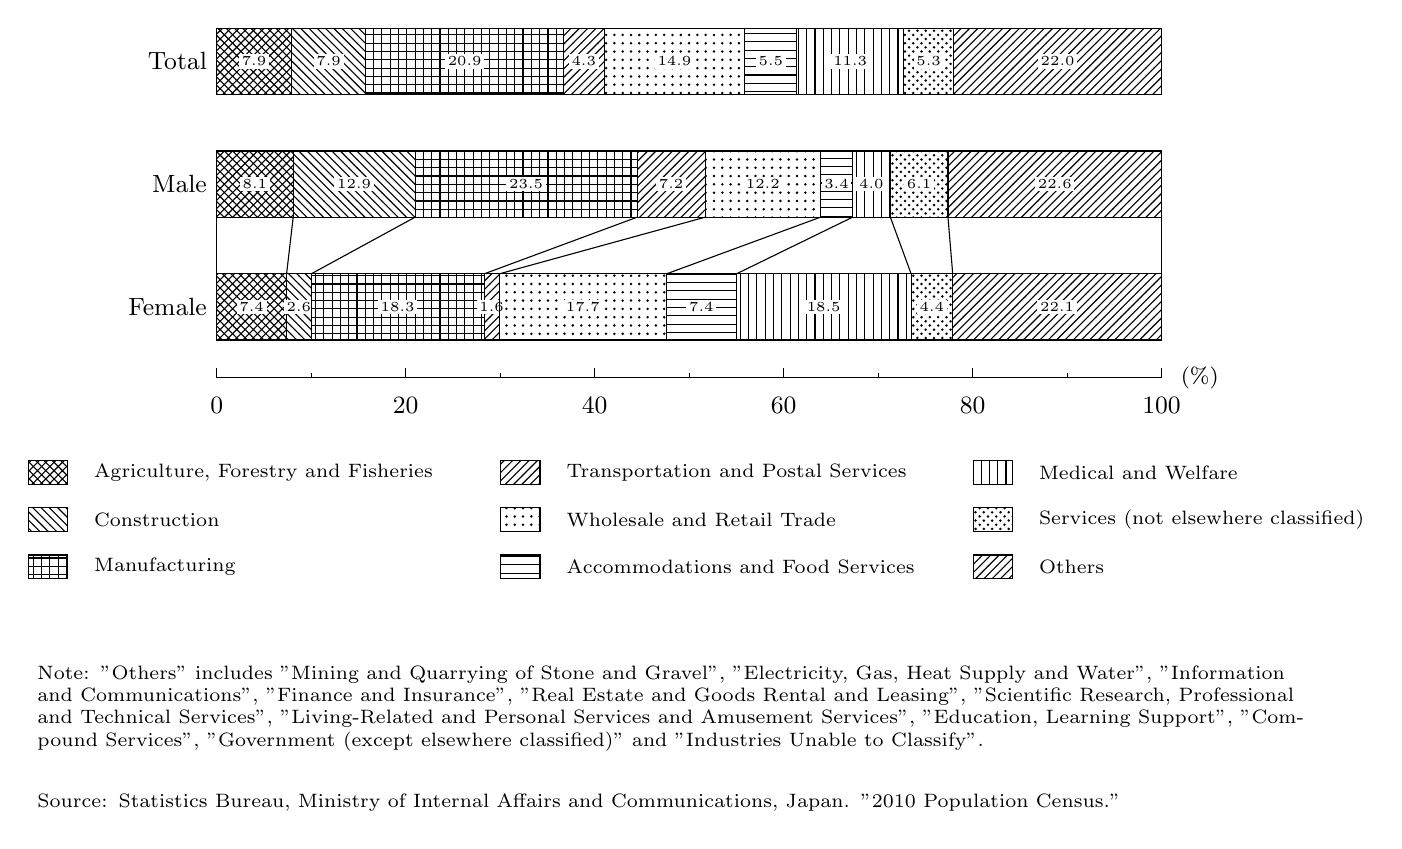
\begin{tikzpicture}[scale=1.20]
\definecolor{color1}{RGB}{200,200,200} 
\definecolor{color2}{RGB}{150,150,150} 
\definecolor{color3}{RGB}{100,100,100}
\definecolor{color4}{RGB}{250,200,200}
\definecolor{color5}{RGB}{200,150,150}
\definecolor{color6}{RGB}{150,100,100}
\definecolor{color7}{RGB}{100,50,50}
\definecolor{color8}{RGB}{50,0,0}
\definecolor{color9}{RGB}{0,0,0}

% Total bar
\draw[fill=color1, pattern=crosshatch] (2,9) rectangle (2.79,9.7) node[pos=0.5, fill=white, inner sep=1pt] {\tiny 7.9};
\draw[fill=color2, pattern=north west lines] (2.79,9) rectangle (3.58,9.7) node[pos=0.5, fill=white, inner sep=1pt] {\tiny 7.9};
\draw[fill=color3, pattern=grid] (3.58,9) rectangle (5.67,9.7) node[pos=0.5, fill=white, inner sep=1pt] {\tiny 20.9};
\draw[fill=color4, pattern=north east lines] (5.67,9) rectangle (6.10,9.7) node[pos=0.5, fill=white, inner sep=1pt] {\tiny 4.3}; 
\draw[fill=color5, pattern=dots] (6.10,9) rectangle (7.59,9.7) node[pos=0.5, fill=white, inner sep=1pt] {\tiny 14.9}; 
\draw[fill=color6, pattern=horizontal lines] (7.59,9) rectangle (8.14,9.7) node[pos=0.5, fill=white, inner sep=1pt] {\tiny 5.5};
\draw[fill=color7, pattern=vertical lines] (8.14,9) rectangle (9.27,9.7) node[pos=0.5, fill=white, inner sep=1pt] {\tiny 11.3};
\draw[fill=color8, pattern=crosshatch dots] (9.27,9) rectangle (9.80,9.7) node[pos=0.5, fill=white, inner sep=1pt] {\tiny 5.3};
\draw[fill=color9, pattern=north east lines] (9.80,9) rectangle (12,9.7) node[pos=0.5, fill=white, inner sep=1pt] {\tiny 22.0}; 

% Male bar
\draw[fill=color1, pattern=crosshatch] (2,7.7) rectangle (2.81,8.4) node[pos=0.5, fill=white, inner sep=1pt] {\tiny 8.1};
\draw[fill=color2, pattern=north west lines] (2.81,7.7) rectangle (4.10,8.4) node[pos=0.5, fill=white, inner sep=1pt] {\tiny 12.9};
\draw[fill=color3, pattern=grid] (4.10,7.7) rectangle (6.45,8.4) node[pos=0.5, fill=white, inner sep=1pt] {\tiny 23.5};
\draw[fill=color4, pattern=north east lines] (6.45,7.7) rectangle (7.17,8.4) node[pos=0.5, fill=white, inner sep=1pt] {\tiny 7.2}; 
\draw[fill=color5, pattern=dots] (7.17,7.7) rectangle (8.39,8.4) node[pos=0.5, fill=white, inner sep=1pt] {\tiny 12.2}; 
\draw[fill=color6, pattern=horizontal lines] (8.39,7.7) rectangle (8.73,8.4) node[pos=0.5, fill=white, inner sep=1pt] {\tiny 3.4};
\draw[fill=color7, pattern=vertical lines] (8.73,7.7) rectangle (9.13,8.4) node[pos=0.5, fill=white, inner sep=1pt] {\tiny 4.0};
\draw[fill=color8, pattern=crosshatch dots] (9.13,7.7) rectangle (9.74,8.4) node[pos=0.5, fill=white, inner sep=1pt] {\tiny 6.1};
\draw[fill=color9, pattern=north east lines] (9.74,7.7) rectangle (12,8.4) node[pos=0.5, fill=white, inner sep=1pt] {\tiny 22.6};

% Female bar
\draw[fill=color1, pattern=crosshatch] (2,6.4) rectangle (2.74,7.1) node[pos=0.5, fill=white, inner sep=1pt] {\tiny 7.4};
\draw[fill=color2, pattern=north west lines] (2.74,6.4) rectangle (3.00,7.1) node[pos=0.5, fill=white, inner sep=1pt] {\tiny 2.6};
\draw[fill=color3, pattern=grid] (3.00,6.4) rectangle (4.83,7.1) node[pos=0.5, fill=white, inner sep=1pt] {\tiny 18.3};
\draw[fill=color4, pattern=north east lines] (4.83,6.4) rectangle (4.99,7.1) node[pos=0.5, fill=white, inner sep=1pt] {\tiny 1.6}; 
\draw[fill=color5, pattern=dots] (4.99,6.4) rectangle (6.76,7.1) node[pos=0.5, fill=white, inner sep=1pt] {\tiny 17.7}; 
\draw[fill=color6, pattern=horizontal lines] (6.76,6.4) rectangle (7.50,7.1) node[pos=0.5, fill=white, inner sep=1pt] {\tiny 7.4};
\draw[fill=color7, pattern=vertical lines] (7.50,6.4) rectangle (9.35,7.1) node[pos=0.5, fill=white, inner sep=1pt] {\tiny 18.5};
\draw[fill=color8, pattern=crosshatch dots] (9.35,6.4) rectangle (9.79,7.1) node[pos=0.5, fill=white, inner sep=1pt] {\tiny 4.4};
\draw[fill=color9, pattern=north east lines] (9.79,6.4) rectangle (12,7.1) node[pos=0.5, fill=white, inner sep=1pt] {\tiny 22.1}; 

% Male to Female guidelines
\draw[thin] (2,7.7) -- (2,7.1);
\draw[thin] (2.81,7.7) -- (2.74,7.1);
\draw[thin] (4.10,7.7) -- (3.00,7.1);
\draw[thin] (6.45,7.7) -- (4.83,7.1);
\draw[thin] (7.17,7.7) -- (4.99,7.1);
\draw[thin] (8.39,7.7) -- (6.76,7.1);
\draw[thin] (8.73,7.7) -- (7.50,7.1);
\draw[thin] (9.13,7.7) -- (9.35,7.1);
\draw[thin] (9.74,7.7) -- (9.79,7.1);
\draw[thin] (12,7.7) -- (12,7.1);

% Labels
\node[anchor=east] at (2,9.35) {\small Total};
\node[anchor=east] at (2,8.05) {\small Male};
\node[anchor=east] at (2,6.75) {\small Female};

% X-axis
\draw (2,6) -- (12,6);
\foreach \x in {0,20,40,60,80,100}
    \draw (2+\x/10,6) -- (2+\x/10,6.1) node[anchor=north] at (2+\x/10,5.9) {\small \x};
\foreach \x in {10,30,50,70,90}
    \draw (2+\x/10,6) -- (2+\x/10,6.05);
\node[anchor=west, font=\footnotesize] at (12.1,6) {(\%)};

% Legend
\node[anchor=west, fill=color1, pattern=crosshatch, minimum width=0.5cm, minimum height=0.3cm, draw] at (0,5) {};
\node[anchor=west] at (0.6,5) {\scriptsize Agriculture, Forestry and Fisheries};
\node[anchor=west, fill=color2, pattern=north west lines, minimum width=0.5cm, minimum height=0.3cm, draw] at (0,4.5) {};
\node[anchor=west] at (0.6,4.5) {\scriptsize Construction};
\node[anchor=west, fill=color3, pattern=grid, minimum width=0.5cm, minimum height=0.3cm, draw] at (0,4) {};
\node[anchor=west] at (0.6,4) {\scriptsize Manufacturing};
\node[anchor=west, fill=color4, pattern=north east lines, minimum width=0.5cm, minimum height=0.3cm, draw] at (5,5) {};
\node[anchor=west] at (5.6,5) {\scriptsize Transportation and Postal Services};
\node[anchor=west, fill=color5, pattern=dots, minimum width=0.5cm, minimum height=0.3cm, draw] at (5,4.5) {};
\node[anchor=west] at (5.6,4.5) {\scriptsize Wholesale and Retail Trade};
\node[anchor=west, fill=color6, pattern=horizontal lines, minimum width=0.5cm, minimum height=0.3cm, draw] at (5,4) {};
\node[anchor=west] at (5.6,4) {\scriptsize Accommodations and Food Services};
\node[anchor=west, fill=color7, pattern=vertical lines, minimum width=0.5cm, minimum height=0.3cm, draw] at (10,5) {};
\node[anchor=west] at (10.6,5) {\scriptsize Medical and Welfare};
\node[anchor=west, fill=color8, pattern=crosshatch dots, minimum width=0.5cm, minimum height=0.3cm, draw] at (10,4.5) {};
\node[anchor=west] at (10.6,4.5) {\scriptsize Services (not elsewhere classified)};
\node[anchor=west, fill=color9, pattern=north east lines, minimum width=0.5cm, minimum height=0.3cm, draw] at (10,4) {};
\node[anchor=west] at (10.6,4) {\scriptsize Others};

% Annotation and Source
\node[text width=16.3cm, anchor=west, font=\scriptsize, align=left] at (0,2.5) {Note: "Others" includes "Mining and Quarrying of Stone and Gravel", "Electricity, Gas, Heat Supply and Water", "Information and Communications", "Finance and Insurance", "Real Estate and Goods Rental and Leasing", "Scientific Research, Professional and Technical Services", "Living-Related and Personal Services and Amusement Services", "Education, Learning Support", "Compound Services", "Government (except elsewhere classified)" and "Industries Unable to Classify".};

\node[text width=16.3cm, anchor=west, font=\scriptsize, align=left] at (0,1.5) {Source: Statistics Bureau, Ministry of Internal Affairs and Communications, Japan. "2010 Population Census."};

\end{tikzpicture} 
\caption{Proportion of Employed Persons Aged 15 and Over by Industry and Sex - Fukushima Pref. (2010)} 
\label{fig:fukushima_employment}

\end{figure}

%%%%%%%%%%%%%%%%%%%%%%%%%%%%%%%%%%%%%%%%%%%%%

%福島県の職業(Occupation)別の男女別15歳以上就業者について、従業上の地位別(Employment type)の割合をみると、全職業(Total)では、男性の場合、「正規の職員・従業員」の割合は「事務従事者」が62.7%だが女性では40.1%である。一方、「パート・アルバイト・その他」の割合は、女性が36.8%に対して男性は9.8%である。自然災害が非正規労働者により大きな負の影響を及ぼすことが知られており、このような雇用形態のジェンダー格差は、そのまま自然災害影響のジェンダーギャップとして現れる。特筆すべきは、農林水産業では73.0%の男性が「Self-employed」と回答しているのに対し、女性の方は81.2%が「Family worker」と回答していることである。つまりFamily businessにおいては夫がオーナーであり、妻はその従業員であるという性別役割分担の存在が見てとれる。これは自然災害時に、夫よりも妻の労働の増減が危機に対する調整弁の役割を果たすことを意味する。

\begin{figure}[!t]
\begin{adjustbox}{width=\textwidth}
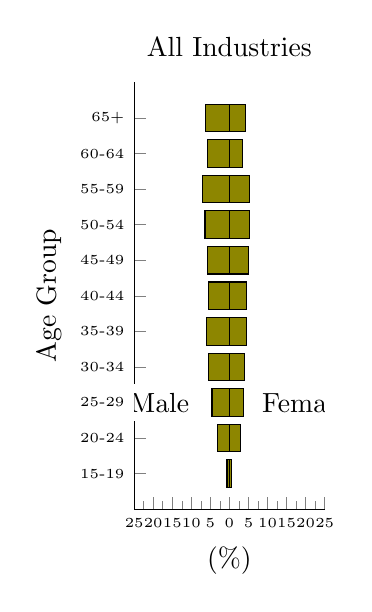
\begin{tikzpicture}
\begin{axis}[
    width=0.33\textwidth,
    height=7cm,
    xbar stacked,
    xmin=-25,
    xmax=25,
    xtick={-25, -20, -15, -10, -5, 0, 5, 10, 15, 20, 25},
    xticklabels={25, 20, 15, 10, 5, 0, 5, 10, 15, 20, 25},
    xlabel={(\%)},
    ylabel={Age Group},
    ytick={1,2,3,4,5,6,7,8,9,10,11},
    yticklabels={15-19, 20-24, 25-29, 30-34, 35-39, 40-44, 45-49, 50-54, 55-59, 60-64, 65+},
    title={All Industries},
    axis y line*=left,
    axis x line*=bottom,
    bar width=3.5mm,
    xticklabel style={font=\tiny},
    yticklabel style={font=\tiny},
    xlabel style={font=\normalsize},
    minor x tick num=1,
    grid style={line width=.1pt, draw=gray!20},
    major grid style={line width=.2pt,draw=gray!50},
]
\addplot[xbar, fill=olive] coordinates {(-6.2968,11) (-5.7348,10) (-7.0630,9) (-6.4160,8) (-5.8457,7) (-5.4109,6) (-6.0469,5) (-5.5079,4) (-4.5710,3) (-3.1366,2) (-0.6502,1)};
\addplot[xbar, fill=olive] coordinates {(4.1861,11) (3.5393,10) (5.1758,9) (5.2826,8) (4.9579,7) (4.4568,6) (4.5115,5) (4.0165,4) (3.6677,3) (2.9304,2) (0.5957,1)};
\node[anchor=east, fill=white] at (axis cs:-8,3) {Male};
\node[anchor=west, fill=white] at (axis cs:6,3) {Female};
\end{axis}
\end{tikzpicture}
\hfill
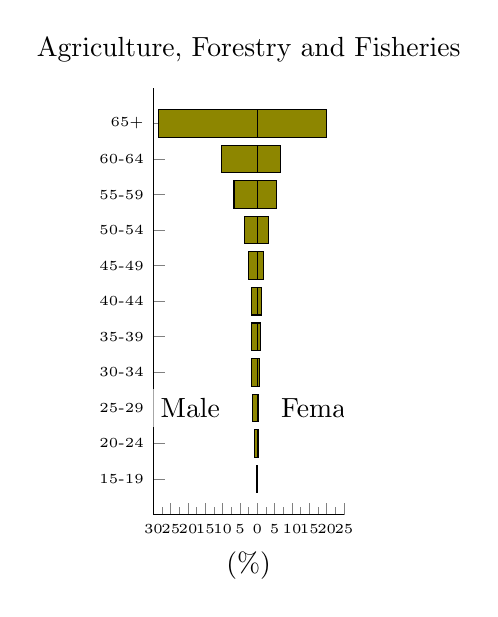
\begin{tikzpicture}
\begin{axis}[
    width=0.33\textwidth,
    height=7cm,
    xbar stacked,
    xmin=-30,
    xmax=25,
    xtick={-30, -25, -20, -15, -10, -5, 0, 5, 10, 15, 20, 25},
    xticklabels={30, 25, 20, 15, 10, 5, 0, 5, 10, 15, 20, 25},
    xlabel={(\%)},
    ytick={1,2,3,4,5,6,7,8,9,10,11},
    yticklabels={15-19, 20-24, 25-29, 30-34, 35-39, 40-44, 45-49, 50-54, 55-59, 60-64, 65+},
    yticklabel pos=right,
    title={Agriculture, Forestry and Fisheries},
    axis y line*=left,
    axis x line*=bottom,
    bar width=3.5mm,
    xticklabel style={font=\tiny},
    yticklabel style={font=\tiny},
    xlabel style={font=\normalsize},
    minor x tick num=1,
    grid style={line width=.1pt, draw=gray!20},
    major grid style={line width=.2pt,draw=gray!50},
]
\addplot[xbar, fill=olive] coordinates {(-28.5896,11) (-10.3951,10) (-6.7607,9) (-3.8248,8) (-2.5634,7) (-1.6352,6) (-1.6058,5) (-1.6520,4) (-1.2908,3) (-0.8218,2) (-0.1694,1)};
\addplot[xbar, fill=olive] coordinates {(20.0734,11) (6.5899,10) (5.5664,9) (3.2718,8) (1.7640,7) (1.1144,6) (0.8792,5) (0.6888,4) (0.4494,3) (0.2394,2) (0.0546,1)};
\node[anchor=east, fill=white] at (axis cs:-8,3) {Male};
\node[anchor=west, fill=white] at (axis cs:4,3) {Female};
\end{axis}
\end{tikzpicture}
\hfill
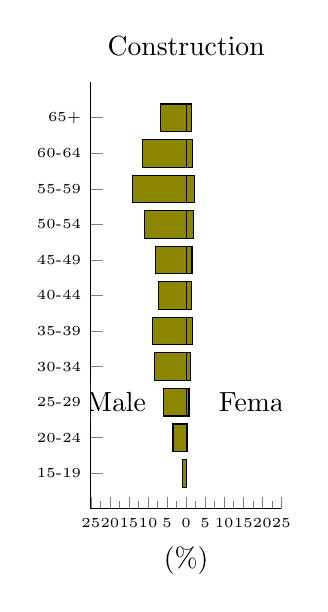
\begin{tikzpicture}
\begin{axis}[
    width=0.33\textwidth,
    height=7cm,
    xbar stacked,
    xmin=-25,
    xmax=25,
    xtick={-25, -20, -15, -10, -5, 0, 5, 10, 15, 20, 25},
    xticklabels={25, 20, 15, 10, 5, 0, 5, 10, 15, 20, 25},
    xlabel={(\%)},
    ytick={1,2,3,4,5,6,7,8,9,10,11},
    yticklabels={15-19, 20-24, 25-29, 30-34, 35-39, 40-44, 45-49, 50-54, 55-59, 60-64, 65+},
    yticklabel pos=right,
    title={Construction},
    axis y line*=left,
    axis x line*=bottom,
    bar width=3.5mm,
    xticklabel style={font=\tiny},
    yticklabel style={font=\tiny},
    xlabel style={font=\normalsize},
    minor x tick num=1,
    grid style={line width=.1pt, draw=gray!20},
    major grid style={line width=.2pt,draw=gray!50},
]
\addplot[xbar, fill=olive] coordinates {(-6.6875,11) (-11.4525,10) (-14.1118,9) (-10.9621,8) (-8.1361,7) (-7.1541,6) (-8.9182,5) (-8.3385,4) (-6.0411,3) (-3.4449,2) (-0.8749,1)};
\addplot[xbar, fill=olive] coordinates {(1.2939,11) (1.7058,10) (2.1069,9) (1.8165,8) (1.5332,7) (1.4439,6) (1.6165,5) (1.2035,4) (0.7380,3) (0.3726,2) (0.0476,1)};
\node[anchor=east, fill=white] at (axis cs:-8,3) {Male};
\node[anchor=west, fill=white] at (axis cs:6,3) {Female};
\end{axis}
\end{tikzpicture}
\end{adjustbox}

% 2行目のグラフ
\begin{adjustbox}{width=\textwidth}
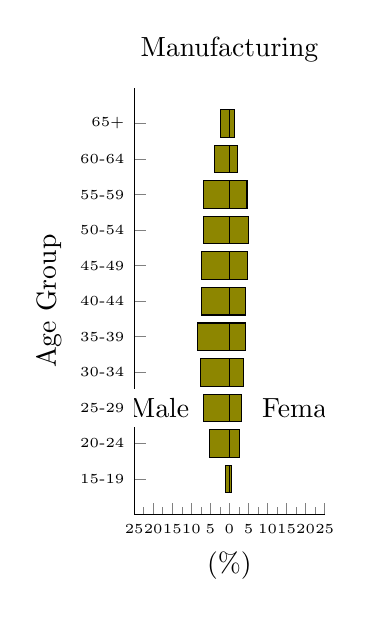
\begin{tikzpicture}
\begin{axis}[
    width=0.33\textwidth,
    height=7cm,
    xbar stacked,
    xmin=-25,
    xmax=25,
    xtick={-25, -20, -15, -10, -5, 0, 5, 10, 15, 20, 25},
    xticklabels={25, 20, 15, 10, 5, 0, 5, 10, 15, 20, 25},
    xlabel={(\%)},
    ylabel={Age Group},
    ytick={1,2,3,4,5,6,7,8,9,10,11},
    yticklabels={15-19, 20-24, 25-29, 30-34, 35-39, 40-44, 45-49, 50-54, 55-59, 60-64, 65+},
    title={Manufacturing},
    axis y line*=left,
    axis x line*=bottom,
    bar width=3.5mm,
    xticklabel style={font=\tiny},
    yticklabel style={font=\tiny},
    xlabel style={font=\normalsize},
    minor x tick num=1,
    grid style={line width=.1pt, draw=gray!20},
    major grid style={line width=.2pt,draw=gray!50},
]
\addplot[xbar, fill=olive] coordinates {(-2.4548,11) (-3.9043,10) (-6.7497,9) (-6.7481,8) (-7.4452,7) (-7.3451,6) (-8.3323,5) (-7.6527,4) (-6.7811,3) (-5.1740,2) (-0.9664,1)};
\addplot[xbar, fill=olive] coordinates {(1.2771,11) (2.1461,10) (4.6067,9) (4.9622,8) (4.8095,7) (4.2896,6) (4.3236,5) (3.6345,4) (3.1567,3) (2.7400,2) (0.5002,1)};
\node[anchor=east, fill=white] at (axis cs:-8,3) {Male};
\node[anchor=west, fill=white] at (axis cs:6,3) {Female};
\end{axis}
\end{tikzpicture}
\hfill
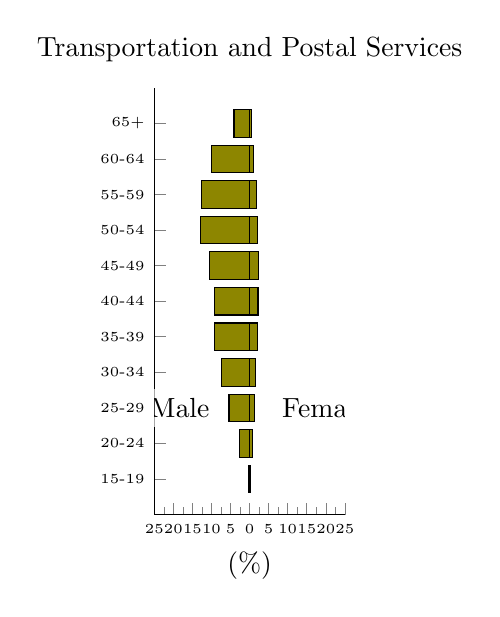
\begin{tikzpicture}
\begin{axis}[
    width=0.33\textwidth,
    height=7cm,
    xbar stacked,
    xmin=-25,
    xmax=25,
    xtick={-25, -20, -15, -10, -5, 0, 5, 10, 15, 20, 25},
    xticklabels={25, 20, 15, 10, 5, 0, 5, 10, 15, 20, 25},
    xlabel={(\%)},
    ytick={1,2,3,4,5,6,7,8,9,10,11},
    yticklabels={15-19, 20-24, 25-29, 30-34, 35-39, 40-44, 45-49, 50-54, 55-59, 60-64, 65+},
    yticklabel pos=right,
    title={Transportation and Postal Services},
    axis y line*=left,
    axis x line*=bottom,
    bar width=3.5mm,
    xticklabel style={font=\tiny},
    yticklabel style={font=\tiny},
    xlabel style={font=\normalsize},
    minor x tick num=1,
    grid style={line width=.1pt, draw=gray!20},
    major grid style={line width=.2pt,draw=gray!50},
]
\addplot[xbar, fill=olive] coordinates {(-4.0825,11) (-10.0013,10) (-12.6223,9) (-12.8891,8) (-10.6053,7) (-9.1725,6) (-9.1152,5) (-7.3627,4) (-5.4052,3) (-2.7445,2) (-0.3836,1)};
\addplot[xbar, fill=olive] coordinates {(0.5070,11) (1.0691,10) (1.8274,9) (2.1030,8) (2.3609,7) (2.2154,6) (2.0787,5) (1.4373,4) (1.1948,3) (0.7164,2) (0.1058,1)};
\node[anchor=east, fill=white] at (axis cs:-8,3) {Male};
\node[anchor=west, fill=white] at (axis cs:6,3) {Female};
\end{axis}
\end{tikzpicture}
\hfill
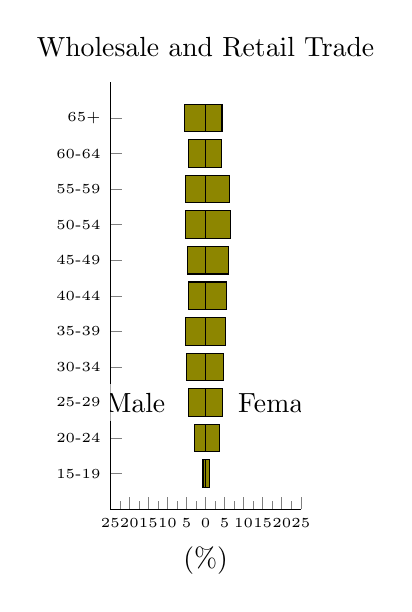
\begin{tikzpicture}
\begin{axis}[
    width=0.33\textwidth,
    height=7cm,
    xbar stacked,
    xmin=-25,
    xmax=25,
    xtick={-25, -20, -15, -10, -5, 0, 5, 10, 15, 20, 25},
    xticklabels={25, 20, 15, 10, 5, 0, 5, 10, 15, 20, 25},
    xlabel={(\%)},
    ytick={1,2,3,4,5,6,7,8,9,10,11},
    yticklabels={15-19, 20-24, 25-29, 30-34, 35-39, 40-44, 45-49, 50-54, 55-59, 60-64, 65+},
    yticklabel pos=right,
    title={Wholesale and Retail Trade},
    axis y line*=left,
    axis x line*=bottom,
    bar width=3.5mm,
    xticklabel style={font=\tiny},
    yticklabel style={font=\tiny},
    xlabel style={font=\normalsize},
    minor x tick num=1,
    grid style={line width=.1pt, draw=gray!20},
    major grid style={line width=.2pt,draw=gray!50},
]
\addplot[xbar, fill=olive] coordinates {(-5.6034,11) (-4.4603,10) (-5.3643,9) (-5.1647,8) (-4.7515,7) (-4.5047,6) (-5.3544,5) (-5.1161,4) (-4.4201,3) (-2.9335,2) (-0.6798,1)};
\addplot[xbar, fill=olive] coordinates {(4.3157,11) (4.1070,10) (6.2549,9) (6.4510,8) (6.0631,7) (5.4397,6) (5.2987,5) (4.7508,4) (4.3911,3) (3.5696,2) (1.0056,1)};
\node[anchor=east, fill=white] at (axis cs:-8,3) {Male};
\node[anchor=west, fill=white] at (axis cs:6,3) {Female};
\end{axis}
\end{tikzpicture}
\end{adjustbox}

% 3行目のグラフ
\begin{adjustbox}{width=\textwidth}
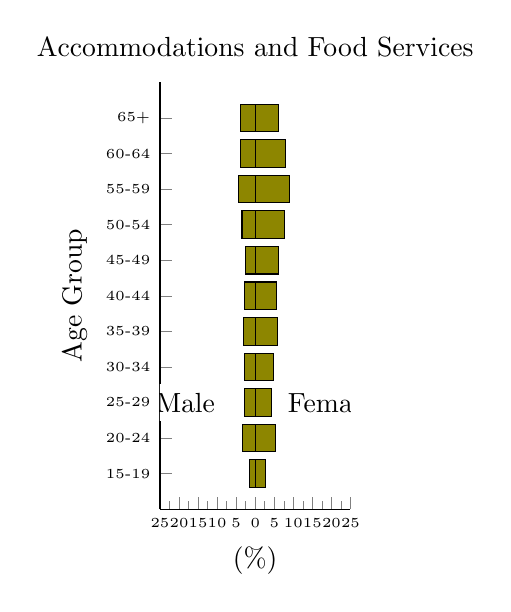
\begin{tikzpicture}
\begin{axis}[
    width=0.33\textwidth,
    height=7cm,
    xbar stacked,
    xmin=-25,
    xmax=25,
    xtick={-25, -20, -15, -10, -5, 0, 5, 10, 15, 20, 25},
    xticklabels={25, 20, 15, 10, 5, 0, 5, 10, 15, 20, 25},
 xlabel={(\%)},
    ylabel={Age Group},
    ytick={1,2,3,4,5,6,7,8,9,10,11},
    yticklabels={15-19, 20-24, 25-29, 30-34, 35-39, 40-44, 45-49, 50-54, 55-59, 60-64, 65+},
    title={Accommodations and Food Services},
    axis y line*=left,
    axis x line*=bottom,
    bar width=3.5mm,
    xticklabel style={font=\tiny},
    yticklabel style={font=\tiny},
    xlabel style={font=\normalsize},
    minor x tick num=1,
    grid style={line width=.1pt, draw=gray!20},
    major grid style={line width=.2pt,draw=gray!50},
]
\addplot[xbar, fill=olive] coordinates {(-3.8505,11) (-3.9093,10) (-4.2855,9) (-3.4547,8) (-2.6611,7) (-2.7884,6) (-3.0647,5) (-2.9217,4) (-2.9119,3) (-3.4410,2) (-1.4697,1)};
\addplot[xbar, fill=olive] coordinates {(6.1236,11) (7.9950,10) (9.0473,9) (7.6775,8) (6.0158,7) (5.6004,6) (5.7866,5) (4.7206,4) (4.3287,3) (5.2163,2) (2.7297,1)};
\node[anchor=east, fill=white] at (axis cs:-8,3) {Male};
\node[anchor=west, fill=white] at (axis cs:6,3) {Female};
\end{axis}
\end{tikzpicture}
\hfill
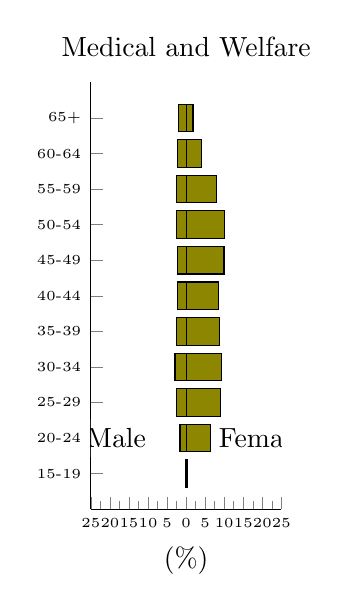
\begin{tikzpicture}
\begin{axis}[
    width=0.33\textwidth,
    height=7cm,
    xbar stacked,
    xmin=-25,
    xmax=25,
    xtick={-25, -20, -15, -10, -5, 0, 5, 10, 15, 20, 25},
    xticklabels={25, 20, 15, 10, 5, 0, 5, 10, 15, 20, 25},
    xlabel={(\%)},
    ytick={1,2,3,4,5,6,7,8,9,10,11},
    yticklabels={15-19, 20-24, 25-29, 30-34, 35-39, 40-44, 45-49, 50-54, 55-59, 60-64, 65+},
    yticklabel pos=right,
    title={Medical and Welfare},
    axis y line*=left,
    axis x line*=bottom,
    bar width=3.5mm,
    xticklabel style={font=\tiny},
    yticklabel style={font=\tiny},
    xlabel style={font=\normalsize},
    minor x tick num=1,
    grid style={line width=.1pt, draw=gray!20},
    major grid style={line width=.2pt,draw=gray!50},
]
\addplot[xbar, fill=olive] coordinates {(-2.0760,11) (-2.1576,10) (-2.4203,9) (-2.4234,8) (-2.3000,7) (-2.1796,6) (-2.5302,5) (-2.9330,4) (-2.5197,3) (-1.6072,2) (-0.1350,1)};
\addplot[xbar, fill=olive] coordinates {(1.8123,11) (4.0820,10) (8.0687,9) (10.0736,8) (9.9229,7) (8.4778,6) (8.8545,5) (9.3578,4) (9.1318,3) (6.4750,2) (0.4615,1)};
\node[anchor=east, fill=white] at (axis cs:-8,2) {Male};
\node[anchor=west, fill=white] at (axis cs:6,2) {Female};
\end{axis}
\end{tikzpicture}
\hfill
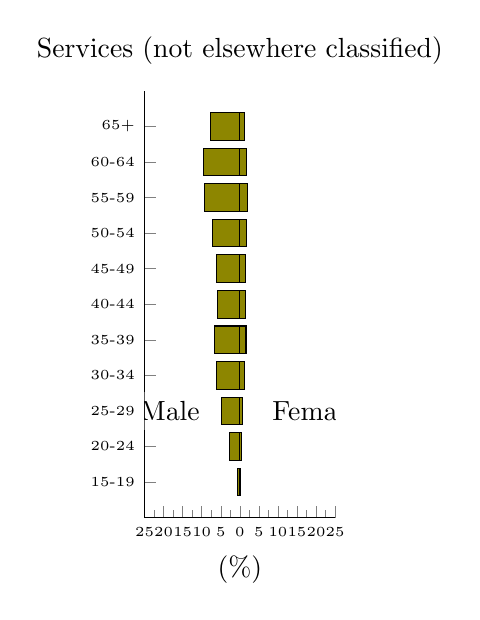
\begin{tikzpicture}
\begin{axis}[
    width=0.33\textwidth,
    height=7cm,
    xbar stacked,
    xmin=-25,
    xmax=25,
    xtick={-25, -20, -15, -10, -5, 0, 5, 10, 15, 20, 25},
    xticklabels={25, 20, 15, 10, 5, 0, 5, 10, 15, 20, 25},
    xlabel={(\%)},
    ytick={1,2,3,4,5,6,7,8,9,10,11},
    yticklabels={15-19, 20-24, 25-29, 30-34, 35-39, 40-44, 45-49, 50-54, 55-59, 60-64, 65+},
    yticklabel pos=right,
    title={Services (not elsewhere classified)},
    axis y line*=left,
    axis x line*=bottom,
    bar width=3.5mm,
    xticklabel style={font=\tiny},
    yticklabel style={font=\tiny},
    xlabel style={font=\normalsize},
    minor x tick num=1,
    grid style={line width=.1pt, draw=gray!20},
    major grid style={line width=.2pt,draw=gray!50},
]
\addplot[xbar, fill=olive] coordinates {(-7.5892,11) (-9.4724,10) (-9.3730,9) (-7.1919,8) (-6.1034,7) (-5.9352,6) (-6.6690,5) (-6.1825,4) (-4.8061,3) (-2.8135,2) (-0.5534,1)};
\addplot[xbar, fill=olive] coordinates {(1.2939,11) (1.7058,10) (2.1069,9) (1.8165,8) (1.5332,7) (1.4439,6) (1.6165,5) (1.2035,4) (0.7380,3) (0.3726,2) (0.0476,1)};
\node[anchor=east, fill=white] at (axis cs:-8,3) {Male};
\node[anchor=west, fill=white] at (axis cs:6,3) {Female};
\end{axis}
\end{tikzpicture}
\end{adjustbox}

\begin{flushleft}
\footnotesize
Source: Statistics Bureau, Ministry of Internal Affairs and Communications, Japan. "2010 Population Census."
\end{flushleft}


\caption{Proportion of Employed Persons Aged 15 and Over by Industry, Age (5-year groups), and Sex - Fukushima Pref. (2010)}
\label{fig:fukushima_Proportion_Employed}
\end{figure}

%%%%%%%%%%%%%%%%%%%%%%%%%%%%%%%%%%%%%%%%%%%%
%Labor force participation rate
%%%%%%%%%%%%%%%%%%%%%%%%%%%%%%%%%%%%%%%%%%%%
\begin{figure}[h!]

\begin{subfigure}{\textwidth}
\caption{Fukushima Pref.}
\begin{minipage}{0.48\textwidth}
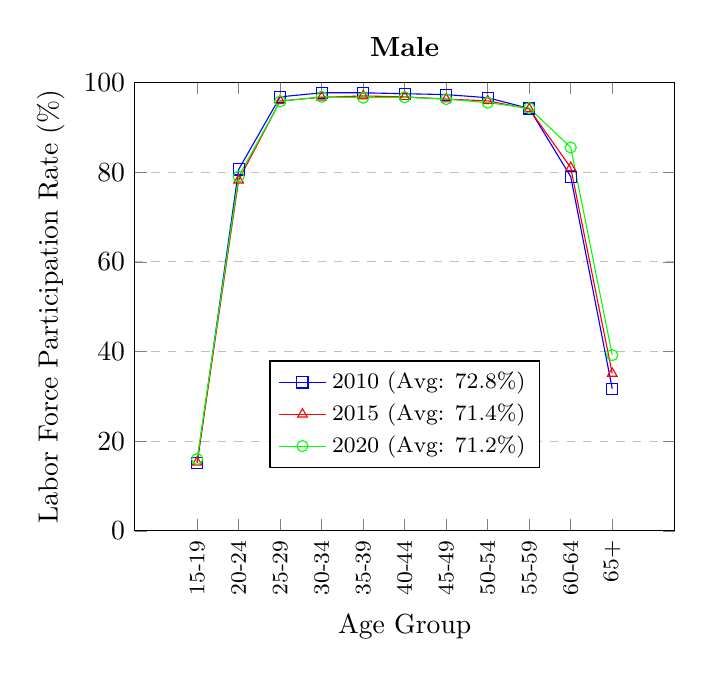
\begin{tikzpicture}
\begin{axis}[
    title={\textbf{Male}},
    xlabel={Age Group},
    ylabel={Labor Force Participation Rate (\%)},
    xmin=0, xmax=12,
    ymin=0, ymax=100,
    xtick={1,2,3,4,5,6,7,8,9,10,11},
    xticklabels={15-19,20-24,25-29,30-34,35-39,40-44,45-49,50-54,55-59,60-64,65+},
    x tick label style={rotate=90,anchor=east,font=\footnotesize},
    legend style={at={(0.5,0.38)},anchor=north,font=\footnotesize,
                  cells={anchor=west},
                  legend columns=1,
                  draw=black,fill=white,align=left},
    ymajorgrids=true,
    grid style=dashed,
    enlarge x limits={abs=0.5},
]

\addplot[color=blue,mark=square,] coordinates {
    (1,15.1)(2,80.6)(3,96.8)(4,97.7)(5,97.7)(6,97.5)(7,97.3)(8,96.6)(9,94.2)(10,79.0)(11,31.7)
};

\addplot[color=red,mark=triangle,] coordinates {
    (1,15.3)(2,78.2)(3,95.9)(4,96.7)(5,97.0)(6,96.8)(7,96.3)(8,95.9)(9,94.1)(10,81.0)(11,35.1)
};

\addplot[color=green,mark=o,] coordinates {
    (1,16.0)(2,79.0)(3,95.8)(4,96.8)(5,96.6)(6,96.7)(7,96.3)(8,95.5)(9,94.3)(10,85.5)(11,39.2)
};

\legend{
    2010 (Avg: 72.8\%),
    2015 (Avg: 71.4\%),
    2020 (Avg: 71.2\%)
}
\end{axis}
\end{tikzpicture}
\end{minipage}
\hfill
\begin{minipage}{0.48\textwidth}
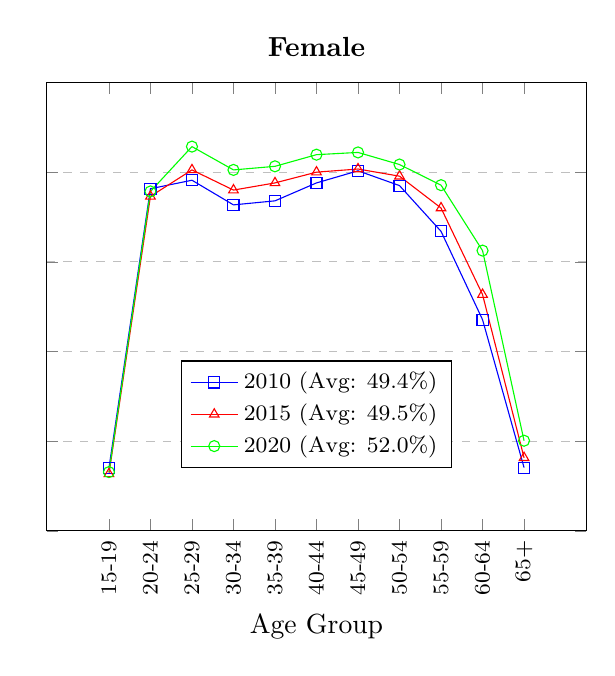
\begin{tikzpicture}
\begin{axis}[
    title={\textbf{Female}},
    xlabel={Age Group},
    ylabel={},
    xmin=0, xmax=12,
    ymin=0, ymax=100,
    xtick={1,2,3,4,5,6,7,8,9,10,11},
    xticklabels={15-19,20-24,25-29,30-34,35-39,40-44,45-49,50-54,55-59,60-64,65+},
    x tick label style={rotate=90,anchor=east,font=\footnotesize},
    legend style={at={(0.5,0.38)},anchor=north,font=\footnotesize,
                  cells={anchor=west},
                  legend columns=1,
                  draw=black,fill=white,align=left},
    ymajorgrids=true,
    grid style=dashed,
    yticklabels={,,},
    enlarge x limits={abs=0.5},
]

\addplot[color=blue,mark=square,] coordinates {
    (1,14.0)(2,76.3)(3,78.2)(4,72.7)(5,73.6)(6,77.6)(7,80.3)(8,77.0)(9,66.8)(10,47.1)(11,14.1)
};

\addplot[color=red,mark=triangle,] coordinates {
    (1,12.7)(2,74.6)(3,80.5)(4,76.0)(5,77.6)(6,80.0)(7,80.7)(8,79.1)(9,72.0)(10,52.7)(11,16.3)
};

\addplot[color=green,mark=o,] coordinates {
    (1,13.1)(2,75.7)(3,85.7)(4,80.5)(5,81.3)(6,83.9)(7,84.4)(8,81.7)(9,77.1)(10,62.5)(11,20.1)
};

\legend{
    2010 (Avg: 49.4\%),
    2015 (Avg: 49.5\%),
    2020 (Avg: 52.0\%)
}
\end{axis}
\end{tikzpicture}
\end{minipage}
\end{subfigure}

\vspace{0.5cm}

\begin{subfigure}{\textwidth}
\caption{Nationwide}
\begin{minipage}{0.48\textwidth}
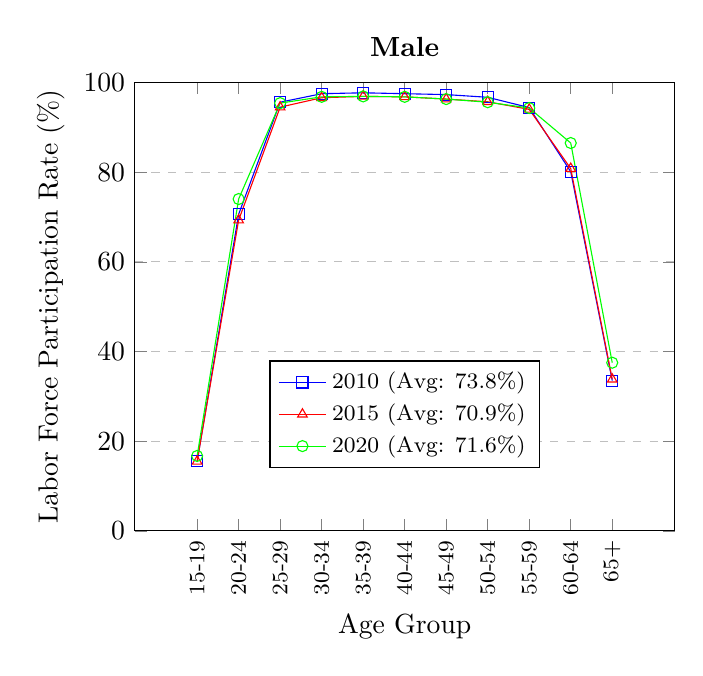
\begin{tikzpicture}
\begin{axis}[
    title={\textbf{Male}},
    xlabel={Age Group},
    ylabel={Labor Force Participation Rate (\%)},
    xmin=0, xmax=12,
    ymin=0, ymax=100,
    xtick={1,2,3,4,5,6,7,8,9,10,11},
    xticklabels={15-19,20-24,25-29,30-34,35-39,40-44,45-49,50-54,55-59,60-64,65+},
    x tick label style={rotate=90,anchor=east,font=\footnotesize},
    legend style={at={(0.5,0.38)},anchor=north,font=\footnotesize,
                  cells={anchor=west},
                  legend columns=1,
                  draw=black,fill=white,align=left},
    ymajorgrids=true,
    grid style=dashed,
    enlarge x limits={abs=0.5},
]

\addplot[color=blue,mark=square,] coordinates {
    (1,15.5)(2,70.6)(3,95.6)(4,97.5)(5,97.7)(6,97.5)(7,97.3)(8,96.7)(9,94.4)(10,80.1)(11,33.5)
};

\addplot[color=red,mark=triangle,] coordinates {
    (1,15.5)(2,69.3)(3,94.5)(4,96.6)(5,96.9)(6,96.8)(7,96.3)(8,95.7)(9,94.0)(10,80.8)(11,33.8)
};

\addplot[color=green,mark=o,] coordinates {
    (1,16.7)(2,74.0)(3,95.4)(4,96.8)(5,96.9)(6,96.8)(7,96.3)(8,95.6)(9,94.3)(10,86.5)(11,37.5)
};

\legend{
    2010 (Avg: 73.8\%),
    2015 (Avg: 70.9\%),
    2020 (Avg: 71.6\%)
}
\end{axis}
\end{tikzpicture}
\end{minipage}
\hfill
\begin{minipage}{0.48\textwidth}
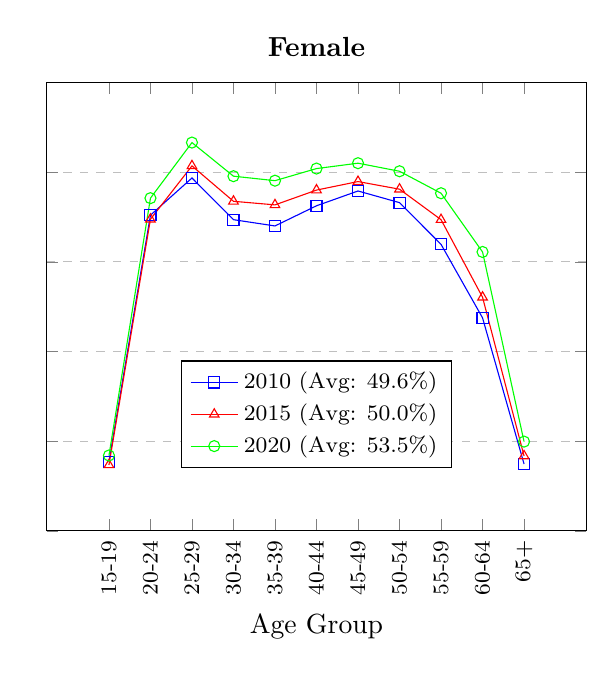
\begin{tikzpicture}
\begin{axis}[
    title={\textbf{Female}},
    xlabel={Age Group},
    ylabel={},
    xmin=0, xmax=12,
    ymin=0, ymax=100,
    xtick={1,2,3,4,5,6,7,8,9,10,11},
    xticklabels={15-19,20-24,25-29,30-34,35-39,40-44,45-49,50-54,55-59,60-64,65+},
    x tick label style={rotate=90,anchor=east,font=\footnotesize},
    legend style={at={(0.5,0.38)},anchor=north,font=\footnotesize,
                  cells={anchor=west},
                  legend columns=1,
                  draw=black,fill=white,align=left},
    ymajorgrids=true,
    grid style=dashed,
    yticklabels={,,},
    enlarge x limits={abs=0.5},
]

\addplot[color=blue,mark=square,] coordinates {
    (1,15.4)(2,70.4)(3,78.7)(4,69.4)(5,68.0)(6,72.5)(7,75.8)(8,73.2)(9,63.9)(10,47.5)(11,14.9)
};

\addplot[color=red,mark=triangle,] coordinates {
    (1,14.7)(2,69.5)(3,81.4)(4,73.5)(5,72.7)(6,76.0)(7,77.9)(8,76.2)(9,69.4)(10,52.1)(11,16.7)
};

\addplot[color=green,mark=o,] coordinates {
    (1,16.8)(2,74.2)(3,86.6)(4,79.1)(5,78.1)(6,80.8)(7,82.0)(8,80.2)(9,75.3)(10,62.2)(11,19.9)
};

\legend{
    2010 (Avg: 49.6\%),
    2015 (Avg: 50.0\%),
    2020 (Avg: 53.5\%)
}
\end{axis}
\end{tikzpicture}
\end{minipage}
\end{subfigure}

\vspace{0.5cm}

\begin{minipage}{\textwidth}
\footnotesize
\textbf{Note:} Labor force participation rates from the 2010, 2015, and 2020 Population Censuses. The ratio of the labor force to the population aged 15 and over (excluding those with "unknown" labor force status).

\end{minipage}

\caption{Labour Force Participation Rate by Age (Five-Year Groups) and Sex - Fukushima/Japan}

\label{fig:fukushima_labour_force_participation_rate}

\end{figure}

%%%%%%%%%%%%%%%%%%%%%%%%%%%%%%%%%%%%%%%%%%%%%
%%%%%%%%%%%%%%%%%%%%%%%%%%%%%%%%%%%%%%%%%%%%%%
% Hello work job openings
%%%%%%%%%%%%%%%%%%%%%%%%%%%%%%%%%%%%%%%%%%%%%%

\begin{figure}[h!]
    \centering
    \includegraphics[width=0.9\textwidth]{New Job Openings.jpeg}  % 幅を本文の80%に設定
    \caption{Hello Work Job Openings and Applicants in Fukushima}
    \label{fig:new_job_openings}
\end{figure}


%Although the number of job openings in the three disaster-affected prefectures of Iwate, Miyagi, and Fukushima initially decreased significantly immediately after the disaster, they have since outperformed the national average. This improvement is largely attributed to the reconstruction demand, including a surge in the construction industry. The first research question of this study investigates how the gender employment gap has evolved under such circumstances.
%%%%%%%%%%%%%%%%%%%%%%%%%%%%%%%%%%%%%%%%%%%%%%


%%%%%%%%%%%%%%%%%%%%%%%%%%%%%%%%%%%%%%%%%%%%%%
%Women ratio on the number of applicants in Fukushima
%%%%%%%%%%%%%%%%%%%%%%%%%%%%%%%%%%%%%%%%%%%%%%
\begin{figure}[h!]
    \centering
    \includegraphics[width=0.9\textwidth]{Women ratio on the number of job applicants.jpg}  % 幅を本文の80%に設定
    \caption{Women ratio on the number of applicants in Fukushima}
    \label{fig:fukushima_Women_ratio_on_applicant}
\end{figure}
%%%%%%%%%%%%%%%%%%%%%%%%%%%%%%%%%%%%%%%%%%%%%%

%%%%%%%%%%%%%%%%%%%%%%%%%%%%%%%%%%%%%%%%%%%%%%
%Women ratio on the number of active job seekers
%%%%%%%%%%%%%%%%%%%%%%%%%%%%%%%%%%%%%%%%%%%%%%

\begin{figure}[h!]
    \centering
    \includegraphics[width=0.9\textwidth]{Women ratio on the number of active job seekers2.jpeg}  % 幅を本文の80%に設定
    \caption{Women ratio on the number of active job seekers in Fukushima}
    \label{fig:women_ratio_fukushima}
\end{figure}


%%%%%%%%%%%%%%%%%%%%%%%%%%%%%%%%%%%%%%%%%%%%%%
%Number of Unemployment Insurance Decisions
%%%%%%%%%%%%%%%%%%%%%%%%%%%%%%%%%%%%%%%%%%%%%%

\begin{figure}[h!]
    \centering
    \includegraphics[width=0.9\textwidth]{Number of Unemployment Insurance decisions.jpg}  % 幅を本文の80%に設定
    \caption{Number of Unemployment Insurance Decisions by Gender in Fukushima}
    \label{fig:employment_insurance_decisions}
\end{figure}

%%%%%%%%%%%%%%%%%%%%%%%%%%%%%%%%%%%%%%%%%%%%%%

%%%%%%%%%%%%%%%%%%%%%%%%%%%%%%%%%%%%%%%%%%%%%%
%Women ratio on the number of Unemployment Insurance Recipients
%%%%%%%%%%%%%%%%%%%%%%%%%%%%%%%%%%%%%%%%%%%%%%

\begin{figure}[h!]
    \centering
    \includegraphics[width=0.9\textwidth]{Number of Actual Unemployment Insurance Recipients2.jpeg}  % 幅を本文の80%に設定
    \caption{Women ratio on the number of Unemployment Insurance Recipients in Fukushima}
    \label{fig:women_ratio_fukushima2}
\end{figure}

%%%%%%%%%%%%%%%%%%%%%%%%%%%%%%%%%%%%%%%%%%%%%%




%%%%%%%%%%%%%%%%%%%%%%%%%%%%%%%%%%%%%%%%%%%%%%
% JGSS analysis
%%%%%%%%%%%%%%%%%%%%%%%%%%%%%%%%%%%%%%%%%%%%%%%%%%

\begin{figure}[ht!]
    \centering
    % Subfigure for the Kernel Density Graph
    \begin{subfigure}[t]{\textwidth}
        \centering
        \includegraphics[width=0.9\textwidth]{Kernel density graphs of respondent’s annual income from main job.png}
        \caption{Kernel density graphs of respondents' annual income from main job (Income bands, $N=20,\!119$)}
        \label{fig:Kernel_density}
    \end{subfigure}
    
    \vspace{1em} % Adds vertical space between the graph and the table

    % Subfigure for the Mean Annual Income Table
    \begin{subfigure}[t]{\textwidth}
        \centering
        \scriptsize
        \setlength{\tabcolsep}{6pt} % Adjust column separation as needed
        \renewcommand{\arraystretch}{1.2} % Increase row height for better readability
        \begin{tabular}{llcccc}
            \toprule
            \multirow{2}{*}{\textbf{Gender}} & \multirow{2}{*}{\textbf{Prefecture}} & \multicolumn{2}{c}{\textbf{Mean Income}} & \multirow{2}{*}{\textbf{Change (\%)}} & \multirow{2}{*}{\textbf{P-value}} \\
            \cmidrule(lr){3-4}
            & & \textbf{Pre} & \textbf{Post} & & \\
            \midrule
            \multirow{2}{*}{Male} 
                & Affected & 7.967 & 7.835 & -1.67 & 0.654 \\
                & Unaffected & 8.660 & 8.300 & \ \quad -4.16*** & 0.000 \\
            \midrule
            \multirow{2}{*}{Female} 
                & Affected & 4.721 & 5.183 & \ +9.79* & 0.065 \\
                & Unaffected & 4.995 & 5.087 & +1.83 & 0.143 \\
            \bottomrule
            \multicolumn{6}{l}{\footnotesize $^{*} p<0.1$, $^{**} p<0.05$, $^{***} p<0.01$}
        \end{tabular}
        \caption{Mean Annual Income from Main Job: Pre/Post-Disaster Period (Income bands, $N=20,\!119$)}
        \label{table:mean_of_annual_income}
    \end{subfigure}
    
    % Main Caption for the Combined Figure and Table
    \caption{Analysis of Respondents' Annual Income from Main Job and Mean Income Changes by Gender and Prefecture}
    \label{fig:combined_figure_table}
\end{figure}

%%%%%%%%%%%%%%%%%%%%%%%%%%%%%%%%%%%%%%%%%%%%%%%%%%%%%%%%%%%%

%%%%%%%%%%%%%%%%%%%%%%%%%%%%%%%%%%%%%%%%%%%%%%
% DID analysis
%%%%%%%%%%%%%%%%%%%%%%%%%%%%%%%%%%%%%%%%%%%%%%%%%%

%%%%%%%%%%%%%%%%%%%%%%%%%%%%%%%%%%%%%%%%%%%%%%%%%%%%
% Placebo_Employment Status%

\begin{table}[htbp]
\centering
\caption{Placebo Test: DID Estimates of Disaster Impact on Employment Status (2000-2005)}

\vspace{-0.2cm}
\resizebox{\linewidth}{!}{%
\begin{tabular}{@{}l*{6}{c}@{}}
          &\multicolumn{3}{c}{Male}                                &\multicolumn{3}{c}{Female}                              \\\cmidrule(lr){2-4}\cmidrule(lr){5-7}
          &\multicolumn{1}{c}{(1)}         &\multicolumn{1}{c}{(2)}         &\multicolumn{1}{c}{(3)}         &\multicolumn{1}{c}{(4)}         &\multicolumn{1}{c}{(5)}         &\multicolumn{1}{c}{(6)}         \\
\toprule
Placebo Disaster Impact (DID)&   -0.014\sym{***}&   -0.011\sym{***}&   -0.013\sym{***}&    0.001         &   -0.004\sym{**} &   -0.004\sym{**} \\
          &  (0.002)         &  (0.002)         &  (0.002)         &  (0.002)         &  (0.002)         &  (0.002)         \\
\addlinespace
Placebo Post-Period&   -0.033\sym{***}&   -0.016\sym{***}&   -0.014\sym{***}&   -0.009\sym{***}&    0.007\sym{***}&    0.006\sym{***}\\
          &  (0.002)         &  (0.002)         &  (0.002)         &  (0.002)         &  (0.002)         &  (0.002)         \\
\addlinespace
Married   &                  &    0.191\sym{***}&    0.118\sym{***}&                  &   -0.098\sym{***}&   -0.062\sym{***}\\
          &                  &  (0.006)         &  (0.004)         &                  &  (0.007)         &  (0.005)         \\
\midrule
Age       &       No         &      Yes         &      Yes         &       No         &      Yes         &      Yes         \\
Relationship with Head&       No         &       No         &      Yes         &       No         &       No         &      Yes         \\
Residence Type&       No         &       No         &      Yes         &       No         &       No         &      Yes         \\
Household Size&       No         &       No         &      Yes         &       No         &       No         &      Yes         \\
$\textit{N}$&   550771         &   550771         &   550771         &   606094         &   606094         &   606094         \\
$\textit{R}^2$&    0.005         &    0.397         &    0.415         &    0.003         &    0.257         &    0.270         \\
Control Mean&    0.707         &    0.707         &    0.707         &    0.471         &    0.471         &    0.471         \\
\bottomrule
\end{tabular}}
\\\multicolumn{7}{@{}p{\linewidth}}{\footnotesize Standard errors clustered at prefecture level in parentheses}\\
\multicolumn{7}{@{}p{\linewidth}}{\footnotesize $*p<0.1$, $**p<0.05$, $***p<0.01$}\\
\multicolumn{7}{@{}p{\linewidth}}{\footnotesize \textit{Note}: This table presents OLS estimates of the placebo disaster impact on employment status for both males and females using 2000 and 2005 population census data. Metropolitan areas (Tokyo, Kanagawa, Saitama, Chiba, Osaka, Kyoto, Hyogo, and Aichi) are excluded from the analysis. Residence Duration is not included as it is unavailable in the 2005 data set. All models include prefecture fixed effects, and the error term is clustered at the prefecture level. The binary variable for marital status assigns 1 to those with a spouse present and 0 to those never married, widowed, or divorced. Control Mean represents the mean employment rate for the control group (non-Fukushima prefectures) in the pre-period (2000).}
\label{table:DID_Employment_Status_Placebo}

\end{table}
%%%%%%%%%%%%%%%%%%%%%%%%%%%%%%%%%%%%%%%%%%%%%%%%%%%%


% ----------------------------------------------------
% Placebo: DID analysis on Regular worker
% ----------------------------------------------------

\begin{table}[htbp]
\centering
\caption{Placebo Test: DID Estimates of Disaster Impact on Regular Worker Status (2000-2005)}

\vspace{-0.2cm}

\resizebox{\linewidth}{!}{%
\begin{tabular}{@{}l*{6}{c}@{}}
          &\multicolumn{3}{c}{Male}                                &\multicolumn{3}{c}{Female}                              \\\cmidrule(lr){2-4}\cmidrule(lr){5-7}
          &\multicolumn{1}{c}{(1)}         &\multicolumn{1}{c}{(2)}         &\multicolumn{1}{c}{(3)}         &\multicolumn{1}{c}{(4)}         &\multicolumn{1}{c}{(5)}         &\multicolumn{1}{c}{(6)}         \\
\toprule
Placebo Disaster Impact (DID)&   -0.009\sym{***}&   -0.007\sym{***}&   -0.009\sym{***}&   -0.005\sym{***}&   -0.009\sym{***}&   -0.009\sym{***}\\
          &  (0.002)         &  (0.002)         &  (0.002)         &  (0.001)         &  (0.001)         &  (0.001)         \\
\addlinespace
Placebo Post-Period&   -0.040\sym{***}&   -0.023\sym{***}&   -0.021\sym{***}&   -0.009\sym{***}&    0.003\sym{**} &    0.000         \\
          &  (0.002)         &  (0.002)         &  (0.002)         &  (0.001)         &  (0.001)         &  (0.001)         \\
\addlinespace
Married   &                  &    0.224\sym{***}&    0.130\sym{***}&                  &   -0.168\sym{***}&   -0.092\sym{***}\\
          &                  &  (0.006)         &  (0.004)         &                  &  (0.006)         &  (0.005)         \\
\midrule
Age Group &       No         &      Yes         &      Yes         &       No         &      Yes         &      Yes         \\
Relationship with Head&       No         &       No         &      Yes         &       No         &       No         &      Yes         \\
Residence Type&       No         &       No         &      Yes         &       No         &       No         &      Yes         \\
Household Size&       No         &       No         &      Yes         &       No         &       No         &      Yes         \\
$\textit{N}$&   550771         &   550771         &   550771         &   606094         &   606094         &   606094         \\
$\textit{R}^2$&    0.006         &    0.383         &    0.400         &    0.003         &    0.214         &    0.224         \\
Control Mean&    0.651         &    0.651         &    0.651         &    0.332         &    0.332         &    0.332         \\
\bottomrule
\end{tabular}}
\\\multicolumn{7}{@{}p{\linewidth}}{\footnotesize Standard errors clustered at prefecture level in parentheses}\\
\multicolumn{7}{@{}p{\linewidth}}{\footnotesize $*p<0.1$, $**p<0.05$, $***p<0.01$}\\
\multicolumn{7}{@{}p{\linewidth}}{\footnotesize \textit{Note}: This table presents OLS estimates of the placebo disaster impact on regular worker status for both males and females using 2000 and 2005 population census data, excluding metropolitan areas. Residence Duration is not included as it is unavailable in the 2005 data set. The occupation variable is also excluded. All models include prefecture fixed effects, and the error term is clustered at the prefecture level. Control Mean represents the average proportion of regular workers in non-Fukushima prefectures before the placebo disaster period.}

\label{tab:placebo_Regular_Worker}

\end{table}

% ----------------------------------------------------

%-------------------------------
%Placebo DID impact on Non-Regular worker status
%-------------------------------

\begin{table}[htbp]
\centering
\caption{Placebo Test: DID Estimates of Disaster Impact on Non-Regular Worker Status (2000-2005)}

\vspace{-0.2cm}

\resizebox{\linewidth}{!}{%
\begin{tabular}{@{}l*{6}{c}@{}}
          &\multicolumn{3}{c}{Male}                                &\multicolumn{3}{c}{Female}                              \\\cmidrule(lr){2-4}\cmidrule(lr){5-7}
          &\multicolumn{1}{c}{(1)}         &\multicolumn{1}{c}{(2)}         &\multicolumn{1}{c}{(3)}         &\multicolumn{1}{c}{(4)}         &\multicolumn{1}{c}{(5)}         &\multicolumn{1}{c}{(6)}         \\
\toprule
Placebo Disaster Impact (DID)&   -0.005\sym{***}&   -0.005\sym{***}&   -0.005\sym{***}&    0.005\sym{***}&    0.005\sym{***}&    0.006\sym{***}\\
          &  (0.001)         &  (0.001)         &  (0.001)         &  (0.001)         &  (0.001)         &  (0.001)         \\
\addlinespace
Placebo Post-Period&    0.007\sym{***}&    0.007\sym{***}&    0.007\sym{***}&    0.000         &    0.004\sym{***}&    0.006\sym{***}\\
          &  (0.001)         &  (0.001)         &  (0.001)         &  (0.001)         &  (0.001)         &  (0.001)         \\
\addlinespace
Married   &                  &   -0.033\sym{***}&   -0.037\sym{***}&                  &    0.070\sym{***}&    0.067\sym{***}\\
          &                  &  (0.001)         &  (0.001)         &                  &  (0.003)         &  (0.003)         \\
\midrule
Age Group &       No         &      Yes         &      Yes         &       No         &      Yes         &      Yes         \\
Residence Type&       No         &       No         &      Yes         &       No         &       No         &      Yes         \\
Relationship with Head&       No         &       No         &      Yes         &       No         &       No         &      Yes         \\
$\textit{N}$&   550771         &   550771         &   550771         &   606094         &   606094         &   606094         \\
$\textit{R}^2$&    0.001         &    0.021         &    0.024         &    0.002         &    0.038         &    0.042         \\
Control Mean&    0.056         &    0.056         &    0.056         &    0.139         &    0.139         &    0.139         \\
\bottomrule
\end{tabular}}
\\\multicolumn{7}{@{}p{\linewidth}}{\footnotesize Standard errors clustered at prefecture level in parentheses}\\
\multicolumn{7}{@{}p{\linewidth}}{\footnotesize $*p<0.1$, $**p<0.05$, $***p<0.01$}\\
\multicolumn{7}{@{}p{\linewidth}}{\footnotesize \textit{Note}: This table reports OLS estimates of the placebo disaster's impact on non-regular worker status for males and females using 2000 and 2005 census data, excluding metropolitan areas, with the sample restricted to the population aged 15 and above. The outcome variable includes individuals categorized as unknown. Occupation variables are excluded. All models include prefecture fixed effects, with standard errors clustered at the prefecture level. Control Mean represents the pre-placebo proportion of non-regular workers in non-Fukushima prefectures.}

\label{table:Placebo_DID_Non_Regular_Worker}

\end{table}

%-------------------------------

%-------------------------------
%Placebo DID impact on Each Employment Type
%-------------------------------

\begin{table}[htbp]
\centering
\caption{Placebo DID Estimates of Disaster Impact on Different Employment Types by Gender}

\vspace{-0.2cm}

\resizebox{\linewidth}{!}{%
\begin{tabular}{@{}l*{17}{c}@{}}
          &\multicolumn{2}{c}{Regular Employee} &\multicolumn{2}{c}{Executive}        &\multicolumn{2}{c}{Self-employed}    &\multicolumn{2}{c}{Dispatched Worker}&\multicolumn{2}{c}{Part-time Worker} &\multicolumn{2}{c}{Family Worker}    &\multicolumn{2}{c}{Unknown Worker}   \\\cmidrule(lr){2-3}\cmidrule(lr){4-5}\cmidrule(lr){6-7}\cmidrule(lr){8-9}\cmidrule(lr){10-11}\cmidrule(lr){12-13}\cmidrule(lr){14-15}
          &\multicolumn{1}{c}{(1)}&\multicolumn{1}{c}{(2)}&\multicolumn{1}{c}{(3)}&\multicolumn{1}{c}{(4)}&\multicolumn{1}{c}{(5)}&\multicolumn{1}{c}{(6)}&\multicolumn{1}{c}{(7)}&\multicolumn{1}{c}{(8)}&\multicolumn{1}{c}{(9)}&\multicolumn{1}{c}{(10)}&\multicolumn{1}{c}{(11)}&\multicolumn{1}{c}{(12)}&\multicolumn{1}{c}{(13)}&\multicolumn{1}{c}{(14)}\\
          &\multicolumn{1}{c}{Male}&\multicolumn{1}{c}{Female}&\multicolumn{1}{c}{Male}&\multicolumn{1}{c}{Female}&\multicolumn{1}{c}{Male}&\multicolumn{1}{c}{Female}&\multicolumn{1}{c}{Male}&\multicolumn{1}{c}{Female}&\multicolumn{1}{c}{Male}&\multicolumn{1}{c}{Female}&\multicolumn{1}{c}{Male}&\multicolumn{1}{c}{Female}&\multicolumn{1}{c}{Male}&\multicolumn{1}{c}{Female}\\
\toprule
Placebo Disaster Impact (DID)&   -0.014\sym{***}&   -0.008\sym{***}&    0.004\sym{***}&   -0.002\sym{***}&   -0.000         &    0.003\sym{***}&   -0.004\sym{***}&    0.003\sym{**} &    0.003\sym{***}&    0.000         &    0.000         &    0.000         &   -0.000\sym{***}&   -0.000\sym{***}\\
          &  (0.002)         &  (0.001)         &  (0.001)         &  (0.001)         &  (0.000)         &  (0.001)         &  (0.001)         &  (0.001)         &  (0.001)         &  (0.000)         &      (.)         &      (.)         &  (0.000)         &  (0.000)         \\
\addlinespace
Post-Placebo Period&   -0.012\sym{***}&    0.008\sym{***}&   -0.009\sym{***}&   -0.005\sym{***}&   -0.002\sym{***}&   -0.008\sym{***}&    0.009\sym{***}&    0.013\sym{***}&   -0.003\sym{***}&   -0.000         &    0.000         &    0.000         &    0.000         &    0.000         \\
          &  (0.002)         &  (0.001)         &  (0.001)         &  (0.001)         &  (0.000)         &  (0.001)         &  (0.001)         &  (0.001)         &  (0.001)         &  (0.000)         &      (.)         &      (.)         &  (0.000)         &  (0.000)         \\
\addlinespace
Married   &    0.147\sym{***}&   -0.145\sym{***}&    0.043\sym{***}&   -0.028\sym{***}&   -0.010\sym{***}&    0.066\sym{***}&   -0.023\sym{***}&    0.004\sym{***}&    0.034\sym{***}&    0.005\sym{***}&    0.000         &    0.000         &   -0.000         &    0.000         \\
          &  (0.006)         &  (0.006)         &  (0.002)         &  (0.001)         &  (0.001)         &  (0.003)         &  (0.001)         &  (0.001)         &  (0.001)         &  (0.000)         &      (.)         &      (.)         &  (0.000)         &  (0.000)         \\
\addlinespace
Age Group &      Yes         &      Yes         &      Yes         &      Yes         &      Yes         &      Yes         &      Yes         &      Yes         &      Yes         &      Yes         &      Yes         &      Yes         &      Yes         &      Yes         \\
\midrule
$\textit{N}$&  550,771         &  606,094         &  550,771         &  606,094         &  550,771         &  606,094         &  550,771         &  606,094         &  550,771         &  606,094         &  550,771         &  606,094         &  550,771         &  606,094         \\
$\textit{R}^2$&    0.349         &    0.223         &    0.062         &    0.016         &    0.006         &    0.041         &    0.025         &    0.030         &    0.024         &    0.008         &        .         &        .         &    0.000         &    0.000         \\
Control Mean&    0.488         &    0.285         &    0.117         &    0.033         &    0.015         &    0.061         &    0.041         &    0.079         &    0.046         &    0.014         &    0.000         &    0.000         &    0.000         &    0.000         \\
\bottomrule
\end{tabular}}
\raggedright
\\\\{\linewidth}{\tiny Standard errors clustered at prefecture level in parentheses}\\\\
\vspace{-0.2cm}
\\\\{\linewidth}{\tiny $*p<0.1$, $**p<0.05$, $***p<0.01$}\\\\
\\\\{\linewidth}{\tiny \textit{Note}: This table presents Placebo DID estimates of the impact of the disaster on different employment types by gender. The dependent variable for each model is a binary indicator for the respective employment type. All models include prefecture fixed effects and age group fixed effects. The error term is clustered at the prefecture level. The binary variable for marital status assigns 1 to those with a spouse present and 0 to those never married, widowed, or divorced. Metropolitan areas (Tokyo, Kanagawa, Saitama, Chiba, Osaka, Kyoto, Hyogo, and Aichi) are excluded from the analysis. Control Mean represents the mean of the dependent variable for the control group (non-Fukushima) in the pre-placebo period.}

\label{table:Placebo_DID_Each_Employment_Type}


\end{table}

%-------------------------------


%%%%%%%%%%%%%%%%%%%%%%%%%%%%%%%%%%%%%%%%%










%%%%%%%%%%%%%%%%%%%%%%%%%%%%%%%%%%%%%%%%%%%%%%%%%%%%%%%%%%%%
\begin{table}[htbp]
\centering
\caption{Difference in the Number of Workers (2010 vs 2015) in Fukushima}
\scriptsize
\begin{tabular}{l *{9}{S[table-format=-5.0]}}
\toprule
\multirow{3}{*}{Occupation} & {\multirow{3}{*}{\makecell[c]{\textbf{Total}\\\underline{(Reg +}\\\underline{Non-reg)}}}} & \multicolumn{4}{c}{\textbf{Regular}} & \multicolumn{4}{c}{\textbf{Non-regular}} \\
\cmidrule(lr){3-6} \cmidrule(lr){7-10}
& & {\multirow{2}{*}{\makecell[c]{\underline{Regular}\\\underline{(Total)}}}} & {Regular} & {Exec.} & {Self-} & {\multirow{2}{*}{\makecell[c]{\underline{Non-reg.}\\\underline{(Total)}}}} & {Disp.} & {Part-time,} & {Family} \\
& & & {empl.} & & {empl.} & & {workers} & {temp.} & {workers} \\
\midrule
\multicolumn{10}{c}{\textbf{Male}} \\
\midrule
Total & 1289 & -545 & 10591 & -1055 & -10081 & 1834 & 870 & 2719 & -1755 \\
Admin. \& managerial & -84 & -28 & -898 & 1296 & -426 & -52 & 0 & -52 & 0 \\
Prof. \& technical & 3521 & 3186 & 3400 & -119 & -95 & 335 & 112 & 263 & -40 \\
Clerical & 9364 & 7612 & 7251 & 276 & 85 & 1752 & 828 & 925 & -1 \\
Sales & -9636 & -8513 & -5186 & -1813 & -1514 & -1123 & -29 & -692 & -402 \\
Service & -1069 & -441 & 395 & -141 & -695 & -628 & 67 & -596 & -99 \\
Security & 1184 & 1094 & 1142 & -1 & -47 & 90 & 0 & 90 & 0 \\
Agri., forest. \& fish. & -6669 & -5959 & -383 & 32 & -5608 & -710 & -16 & -6 & -688 \\
Manufacturing & -14864 & -12017 & -10002 & -614 & -1401 & -2847 & -1668 & -768 & -411 \\
Trans. \& machine op. & 1042 & 596 & 747 & 19 & -170 & 446 & 122 & 308 & 16 \\
Constr. \& mining & 13740 & 11435 & 11403 & 85 & -53 & 2319 & 0 & 2211 & 108 \\
Carrying, clean., pack. & 7279 & 4519 & 4291 & -67 & 295 & 2760 & 1657 & 1179 & -76 \\
Not Classifiable & -2569 & -2049 & -1569 & 2 & -482 & -520 & -209 & -153 & -158 \\
\midrule
\multicolumn{10}{c}{\textbf{Female}} \\
\midrule
Total & -14626 & -1518 & 208 & 24 & -1750 & -13108 & -194 & -5413 & -7501 \\
Admin. \& managerial & 141 & 173 & -131 & 337 & -33 & -14 & 0 & -14 & 0 \\
Prof. \& technical & 2629 & 1957 & 2245 & 48 & -336 & 672 & -114 & 872 & -86 \\
Clerical & 4734 & 2516 & 2034 & 384 & 98 & 2218 & 921 & 1541 & -244 \\
Sales & -6188 & -2072 & -1053 & -489 & -530 & -4116 & -184 & -2580 & -1352 \\
Service & -2922 & 284 & 1496 & -140 & -1072 & -3206 & 27 & -2359 & -874 \\
Security & -33 & 87 & 72 & 8 & 7 & -120 & 0 & -120 & 0 \\
Agri., forest. \& fish. & -3950 & -127 & 10 & -17 & -120 & -3823 & -16 & -53 & -3754 \\
Manufacturing & -8632 & -4003 & -3494 & -73 & -436 & -4629 & -765 & -3236 & -628 \\
Trans. \& machine op. & 103 & 78 & 29 & -7 & 56 & 25 & -20 & 59 & -14 \\
Constr. \& mining & 328 & 96 & 124 & -27 & -1 & 222 & 0 & 208 & 14 \\
Carrying, clean., pack. & 646 & 12 & -329 & 33 & 308 & 634 & 26 & 537 & 71 \\
Not Classifiable & -1502 & -519 & -795 & -33 & 309 & -983 & -89 & -278 & -616 \\
\bottomrule
\end{tabular}

\addlinespace[0.35em]

\raggedright
\scriptsize
\textit{Note}: This table presents changes in the number of workers aged 15 years and over in Fukushima Prefecture between 2010 and 2015. The data is reorganized from the original census categories, which include regular employees, dispatched workers, part-time workers, executives, self-employed (with and without employees), family workers, and home-based workers. Workers with unclassifiable employment status are excluded from this analysis.\\
\textit{Source}: 2010 and 2015 Population Census.\\
\label{table:difference_workers_fukushima}
\end{table}
%%%%%%%%%%%%%%%%%%%%%%%%%%%%%%%%%%%%%%%%%%%%%%%%%%%%%%%%%%%%

%%%%%%%%%%%%%%%%%%%%%%%%%%
%Employment categories

\begin{table}[htbp]
\centering
\caption{Employment Types Used in Population Census and Study Classification}
\small
\begin{tabular}{>{\raggedright\arraybackslash}p{0.3\textwidth}>{\raggedright\arraybackslash}p{0.4\textwidth}>{\raggedright\arraybackslash}p{0.2\textwidth}}
\toprule
\textbf{Census Category} & \textbf{Definition} & \textbf{Study Classification} \\
\midrule
Regular employees & Regular employee has an indefinite employment contract with the employer. & \multirow{3}{*}{Regular workers} \\
\cmidrule{1-2}
Executives & Directors of a company or a corporation including managing directors. & \\
\cmidrule{1-2}
Self-employed & Persons who ran a business with or without employees. & \\
\midrule
Dispatched workers from temporary labour agency & Dispatched worker from temporary labour agency based on relevant low. & \multirow{3}{*}{Non-regular workers} \\
\cmidrule{1-2}
Part-time/temporary employees and others & "Part-time worker", "Arbeit (temporary worker)" and "Contract employee or entrusted employee". & \\
\cmidrule{1-2}
Family workers & Persons who worked in a business operated by a member of the household in which they lived. & \\
\bottomrule
\end{tabular}
\label{tab:employment_status}
\begin{flushleft}
\footnotesize
\textit{Note}: This table shows the employment type categories used in the Population Census and how I classified in this study. "Self-employed" combines both categories of self-employed (with and without employees) from the census. "Persons doing home handicraft" from the census are included in the "Family workers" category.\\
\textit{Source}: Adapted from Statistics Bureau of Japan, Population Census webpage: \url{https://www.stat.go.jp/english/data/kokusei/index.html}
\end{flushleft}

\label{table:employment_category}

\end{table}

%%%%%%%%%%%%%%%%%%%%%%%%%%



%%%%%%%%%%%%%%%%%%%%%%%%%%%%%%%%%



\thispagestyle{empty} % このページのページ番号を消す
%%%%%%%%%%%%%%%%%%%%%%%%%%%%%%%%%

\begin{figure}[htbp]

\centering

% 2010 Figure

\begin{subfigure}{\textwidth}
\centering
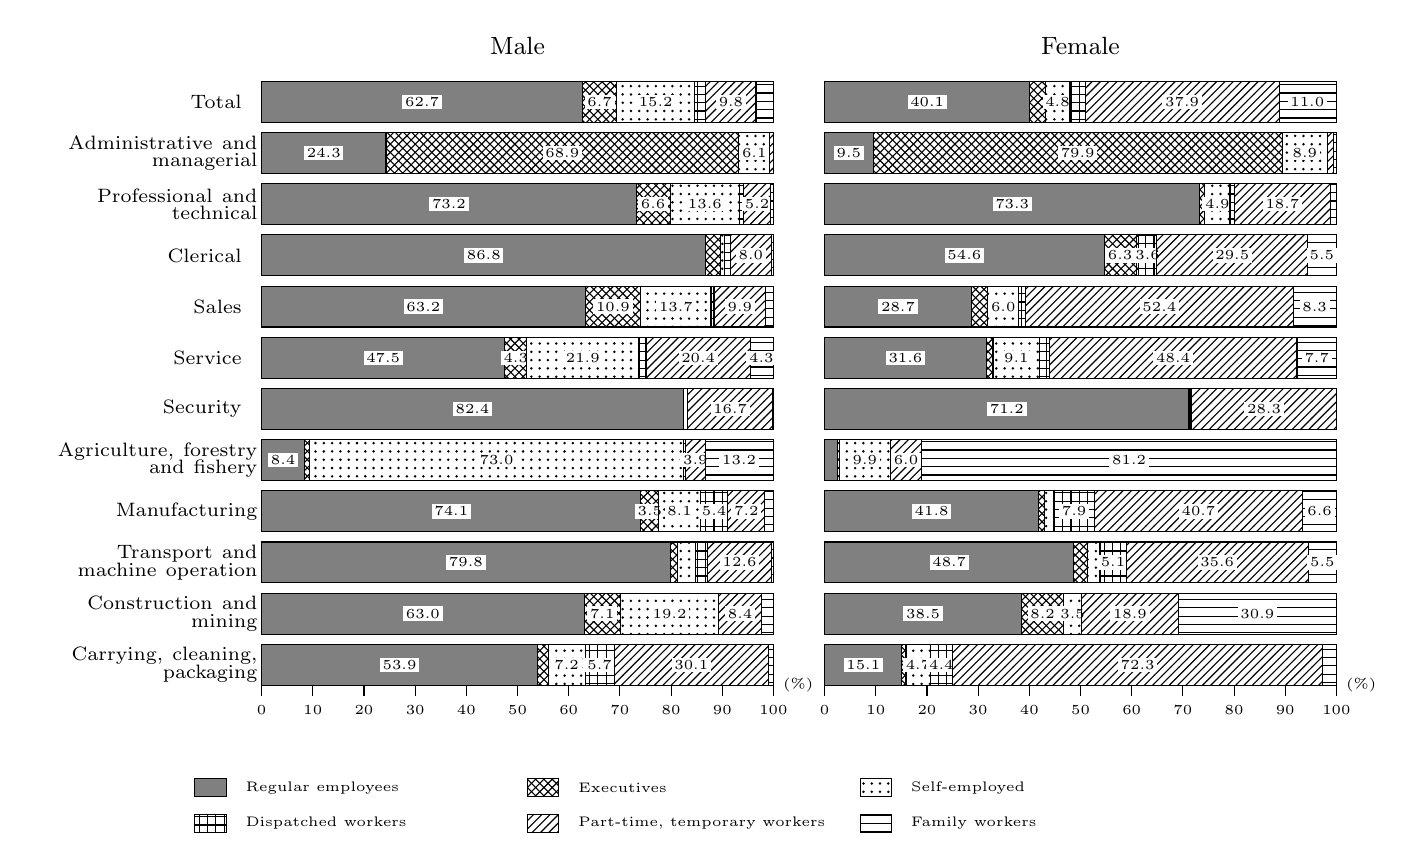
\begin{tikzpicture}[scale=0.65,xshift=-2cm]

\definecolor{color1}{RGB}{128,128,128}
\definecolor{color2}{RGB}{200,200,200}
\definecolor{color3}{RGB}{220,220,220}
\definecolor{color4}{RGB}{180,180,180}
\definecolor{color5}{RGB}{100,100,100}
\definecolor{color6}{RGB}{60,60,60}

% Function to draw a stacked bar
\newcommand{\stackedbar}[8]{
    \draw[fill=color1] (#1,#2) rectangle (#1+#3/10,#2+0.8);
    \pgfmathsetmacro{\result}{(#3 >= 3.5) ? 1 : 0}
    \ifnum\result>0
        \node[font=\tiny,fill=white,text=black,inner sep=1pt] at (#1+#3/20,#2+0.4) {#3};
    \fi
    \draw[fill=color2, pattern=crosshatch] (#1+#3/10,#2) rectangle (#1+#3/10+#4/10,#2+0.8);
    \pgfmathsetmacro{\result}{(#4 >= 3.5) ? 1 : 0}
    \ifnum\result>0
        \node[font=\tiny,fill=white,text=black,inner sep=1pt] at (#1+#3/10+#4/20,#2+0.4) {#4};
    \fi
    \draw[fill=color3, pattern=dots] (#1+#3/10+#4/10,#2) rectangle (#1+#3/10+#4/10+#5/10,#2+0.8);
    \pgfmathsetmacro{\result}{(#5 >= 3.5) ? 1 : 0}
    \ifnum\result>0
        \node[font=\tiny,fill=white,text=black,inner sep=1pt] at (#1+#3/10+#4/10+#5/20,#2+0.4) {#5};
    \fi
    \draw[fill=color4, pattern=grid] (#1+#3/10+#4/10+#5/10,#2) rectangle (#1+#3/10+#4/10+#5/10+#6/10,#2+0.8);
    \pgfmathsetmacro{\result}{(#6 >= 3.5) ? 1 : 0}
    \ifnum\result>0
        \node[font=\tiny,fill=white,text=black,inner sep=1pt] at (#1+#3/10+#4/10+#5/10+#6/20,#2+0.4) {#6};
    \fi
    \draw[fill=color5, pattern=north east lines] (#1+#3/10+#4/10+#5/10+#6/10,#2) rectangle (#1+#3/10+#4/10+#5/10+#6/10+#7/10,#2+0.8);
    \pgfmathsetmacro{\result}{(#7 >= 3.5) ? 1 : 0}
    \ifnum\result>0
        \node[font=\tiny,fill=white,text=black,inner sep=1pt] at (#1+#3/10+#4/10+#5/10+#6/10+#7/20,#2+0.4) {#7};
    \fi
    \draw[fill=color6, pattern=horizontal lines] (#1+#3/10+#4/10+#5/10+#6/10+#7/10,#2) rectangle (#1+10,#2+0.8);
    \pgfmathsetmacro{\result}{(#8 >= 3.5) ? 1 : 0}
    \ifnum\result>0
        \node[font=\tiny,fill=white,text=black,inner sep=1pt] at (#1+#3/10+#4/10+#5/10+#6/10+#7/10+#8/20,#2+0.4) {#8};
    \fi
}

% Male bars
\begin{scope}[xshift=-5.5cm]
\stackedbar{0}{11}{62.7}{6.7}{15.2}{2.2}{9.8}{2.3}
\node[anchor=east, text width=2.6cm, align=right] at (-0.2,11.4) {\scriptsize Total};
\stackedbar{0}{10}{24.3}{68.9}{6.1}{0}{0.7}{0}
\node[anchor=east, text width=2.6cm, align=right] at (-0.2,10.4) {\scriptsize\parbox[t]{2.8cm}{\setstretch{0.8}\raggedleft Administrative and managerial}};
\stackedbar{0}{9}{73.2}{6.6}{13.6}{0.8}{5.2}{0.6}
\node[anchor=east, text width=2.6cm, align=right] at (-0.2,9.4) {\scriptsize\parbox[t]{2.8cm}{\setstretch{0.8}\raggedleft Professional and technical}};
\stackedbar{0}{8}{86.8}{2.9}{0.7}{1.2}{8.0}{0.3}
\node[anchor=east, text width=2.6cm, align=right] at (-0.2,8.4) {\scriptsize Clerical};
\stackedbar{0}{7}{63.2}{10.9}{13.7}{0.7}{9.9}{1.6}
\node[anchor=east, text width=2.6cm, align=right] at (-0.2,7.4) {\scriptsize Sales};
\stackedbar{0}{6}{47.5}{4.3}{21.9}{1.4}{20.4}{4.3}
\node[anchor=east, text width=2.6cm, align=right] at (-0.2,6.4) {\scriptsize Service};
\stackedbar{0}{5}{82.4}{0.1}{0.7}{0}{16.7}{0}
\node[anchor=east, text width=2.6cm, align=right] at (-0.2,5.4) {\scriptsize Security};
\stackedbar{0}{4}{8.4}{1.0}{73.0}{0.4}{3.9}{13.2}
\node[anchor=east, text width=2.6cm, align=right] at (-0.2,4.4) {\scriptsize\parbox[t]{2.8cm}{\setstretch{0.8}\raggedleft Agriculture, forestry and fishery}};
\stackedbar{0}{3}{74.1}{3.5}{8.1}{5.4}{7.2}{1.5}
\node[anchor=east, text width=2.6cm, align=right] at (-0.2,3.4) {\scriptsize\parbox[t]{2.8cm}{\setstretch{0.8}\raggedleft Manufacturing}};
\stackedbar{0}{2}{79.8}{1.5}{3.4}{2.4}{12.6}{0.2}
\node[anchor=east, text width=2.6cm, align=right] at (-0.2,2.4) {\scriptsize\parbox[t]{2.8cm}{\setstretch{0.8}\raggedleft Transport and machine operation}};
\stackedbar{0}{1}{63.0}{7.1}{19.2}{0}{8.4}{2.2}
\node[anchor=east, text width=2.6cm, align=right] at (-0.2,1.4) {\scriptsize\parbox[t]{2.8cm}{\setstretch{0.8}\raggedleft Construction and mining}};
\stackedbar{0}{0}{53.9}{2.1}{7.2}{5.7}{30.1}{1.0}
\node[anchor=east, text width=2.6cm, align=right] at (-0.2,0.4) {\scriptsize\parbox[t]{2.8cm}{\setstretch{0.8}\raggedleft Carrying, cleaning, packaging}};

% X-axis for Male
\draw (0,0) -- (10,0);
\foreach \x in {0,1,...,10}
    \draw (\x,0) -- (\x,-0.2) node[anchor=north] {\tiny \ifnum\x=0 0\else\x0\fi};
\node[anchor=west] at (10,0) {\tiny (\%)};

% Label for Male
\node[anchor=center] at (5,12.5) {\small Male};
\end{scope}

% Female bars
\begin{scope}[xshift=5.5cm]
\stackedbar{0}{11}{40.1}{3.0}{4.8}{3.0}{37.9}{11.0}
\stackedbar{0}{10}{9.5}{79.9}{8.9}{0}{1.1}{0.6}
\stackedbar{0}{9}{73.3}{1.0}{4.9}{0.9}{18.7}{1.2}
\stackedbar{0}{8}{54.6}{6.3}{0.4}{3.6}{29.5}{5.5}
\stackedbar{0}{7}{28.7}{3.2}{6.0}{1.3}{52.4}{8.3}
\stackedbar{0}{6}{31.6}{1.3}{9.1}{1.9}{48.4}{7.7}
\stackedbar{0}{5}{71.2}{0.2}{0.3}{0}{28.3}{0}
\stackedbar{0}{4}{2.5}{0.4}{9.9}{0.1}{6.0}{81.2}
\stackedbar{0}{3}{41.8}{1.1}{1.9}{7.9}{40.7}{6.6}
\stackedbar{0}{2}{48.7}{2.7}{2.4}{5.1}{35.6}{5.5}
\stackedbar{0}{1}{38.5}{8.2}{3.5}{0}{18.9}{30.9}
\stackedbar{0}{0}{15.1}{0.8}{4.7}{4.4}{72.3}{2.8}

% X-axis for Female
\draw (0,0) -- (10,0);
\foreach \x in {0,1,...,10}
    \draw (\x,0) -- (\x,-0.2) node[anchor=north] {\tiny \ifnum\x=0 0\else\x0\fi};
\node[anchor=west] at (10,0) {\tiny (\%)};

% Label for Female
\node[anchor=center] at (5,12.5) {\small Female};
\end{scope}

% Legend (2 rows, 3 columns)
\node[anchor=center, fill=color1, minimum width=0.4cm, minimum height=0.2cm, draw] at (-6.5,-2) {};
\node[anchor=west] at (-6,-2) {\tiny Regular employees};
\node[anchor=center, fill=color2, pattern=crosshatch, minimum width=0.4cm, minimum height=0.2cm, draw] at (0,-2) {};
\node[anchor=west] at (0.5,-2) {\tiny Executives};
\node[anchor=center, fill=color3, pattern=dots, minimum width=0.4cm, minimum height=0.2cm, draw] at (6.5,-2) {};
\node[anchor=west] at (7,-2) {\tiny Self-employed};
\node[anchor=center, fill=color4, pattern=grid, minimum width=0.4cm, minimum height=0.2cm, draw] at (-6.5,-2.7) {};
\node[anchor=west] at (-6,-2.7) {\tiny Dispatched workers};
\node[anchor=center, fill=color5, pattern=north east lines, minimum width=0.4cm, minimum height=0.2cm, draw] at (0,-2.7) {};
\node[anchor=west] at (0.5,-2.7) {\tiny Part-time, temporary workers};
\node[anchor=center, fill=color6, pattern=horizontal lines, minimum width=0.4cm, minimum height=0.2cm, draw] at (6.5,-2.7) {};
\node[anchor=west] at (7,-2.7) {\tiny Family workers};

\end{tikzpicture}
\caption{2010}
\label{fig:proportion_2010}
\end{subfigure}

%%%%%%%%%%%%%%%%%%%%%%%%%%%%%%%%%
\vspace{0.25cm} % 1cm分のスペースを空ける
%%%%%%%%%%%%%%%%%%%%%%%%%%%%%%%%%


% 2015 Figure

\begin{subfigure}{\textwidth}
\centering
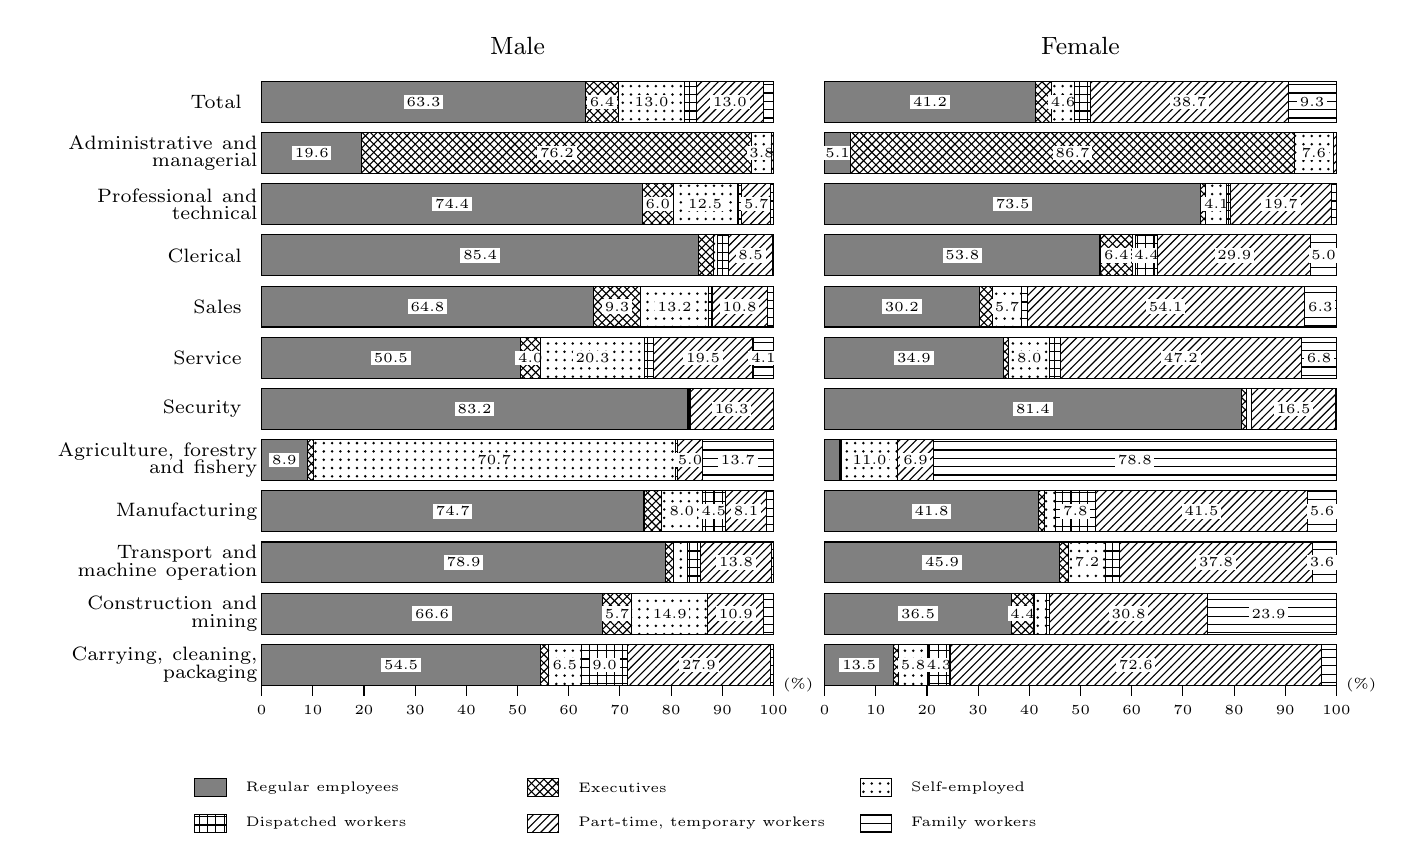
\begin{tikzpicture}
[scale=0.65,xshift=-2cm]
\definecolor{color1}{RGB}{128,128,128}
\definecolor{color2}{RGB}{200,200,200}
\definecolor{color3}{RGB}{220,220,220}
\definecolor{color4}{RGB}{180,180,180}
\definecolor{color5}{RGB}{100,100,100}
\definecolor{color6}{RGB}{60,60,60}

% Function to draw a stacked bar
\newcommand{\stackedbar}[8]{
    \draw[fill=color1] (#1,#2) rectangle (#1+#3/10,#2+0.8);
    \pgfmathsetmacro{\result}{(#3 >= 3.5) ? 1 : 0}
    \ifnum\result>0
        \node[font=\tiny,fill=white,text=black,inner sep=1pt] at (#1+#3/20,#2+0.4) {#3};
    \fi
    \draw[fill=color2, pattern=crosshatch] (#1+#3/10,#2) rectangle (#1+#3/10+#4/10,#2+0.8);
    \pgfmathsetmacro{\result}{(#4 >= 3.5) ? 1 : 0}
    \ifnum\result>0
        \node[font=\tiny,fill=white,text=black,inner sep=1pt] at (#1+#3/10+#4/20,#2+0.4) {#4};
    \fi
    \draw[fill=color3, pattern=dots] (#1+#3/10+#4/10,#2) rectangle (#1+#3/10+#4/10+#5/10,#2+0.8);
    \pgfmathsetmacro{\result}{(#5 >= 3.5) ? 1 : 0}
    \ifnum\result>0
        \node[font=\tiny,fill=white,text=black,inner sep=1pt] at (#1+#3/10+#4/10+#5/20,#2+0.4) {#5};
    \fi
    \draw[fill=color4, pattern=grid] (#1+#3/10+#4/10+#5/10,#2) rectangle (#1+#3/10+#4/10+#5/10+#6/10,#2+0.8);
    \pgfmathsetmacro{\result}{(#6 >= 3.5) ? 1 : 0}
    \ifnum\result>0
        \node[font=\tiny,fill=white,text=black,inner sep=1pt] at (#1+#3/10+#4/10+#5/10+#6/20,#2+0.4) {#6};
    \fi
    \draw[fill=color5, pattern=north east lines] (#1+#3/10+#4/10+#5/10+#6/10,#2) rectangle (#1+#3/10+#4/10+#5/10+#6/10+#7/10,#2+0.8);
    \pgfmathsetmacro{\result}{(#7 >= 3.5) ? 1 : 0}
    \ifnum\result>0
        \node[font=\tiny,fill=white,text=black,inner sep=1pt] at (#1+#3/10+#4/10+#5/10+#6/10+#7/20,#2+0.4) {#7};
    \fi
    \draw[fill=color6, pattern=horizontal lines] (#1+#3/10+#4/10+#5/10+#6/10+#7/10,#2) rectangle (#1+10,#2+0.8);
    \pgfmathsetmacro{\result}{(#8 >= 3.5) ? 1 : 0}
    \ifnum\result>0
        \node[font=\tiny,fill=white,text=black,inner sep=1pt] at (#1+#3/10+#4/10+#5/10+#6/10+#7/10+#8/20,#2+0.4) {#8};
    \fi
}

% Male bars
\begin{scope}[xshift=-5.5cm]
\stackedbar{0}{11}{63.3}{6.4}{13.0}{2.3}{13.0}{1.9}
\node[anchor=east, text width=2.6cm, align=right] at (-0.2,11.4) {\scriptsize Total};
\stackedbar{0}{10}{19.6}{76.2}{3.8}{0.0}{0.4}{0.0}
\node[anchor=east, text width=2.6cm, align=right] at (-0.2,10.4) {\scriptsize\parbox[t]{2.8cm}{\setstretch{0.8}\raggedleft Administrative and managerial}};
\stackedbar{0}{9}{74.4}{6.0}{12.5}{0.9}{5.7}{0.5}
\node[anchor=east, text width=2.6cm, align=right] at (-0.2,9.4) {\scriptsize\parbox[t]{2.8cm}{\setstretch{0.8}\raggedleft Professional and technical}};
\stackedbar{0}{8}{85.4}{2.9}{0.7}{2.3}{8.5}{0.3}
\node[anchor=east, text width=2.6cm, align=right] at (-0.2,8.4) {\scriptsize Clerical};
\stackedbar{0}{7}{64.8}{9.3}{13.2}{0.7}{10.8}{1.1}
\node[anchor=east, text width=2.6cm, align=right] at (-0.2,7.4) {\scriptsize Sales};
\stackedbar{0}{6}{50.5}{4.0}{20.3}{1.7}{19.5}{4.1}
\node[anchor=east, text width=2.6cm, align=right] at (-0.2,6.4) {\scriptsize Service};
\stackedbar{0}{5}{83.2}{0.1}{0.4}{0.0}{16.3}{0.0}
\node[anchor=east, text width=2.6cm, align=right] at (-0.2,5.4) {\scriptsize Security};
\stackedbar{0}{4}{8.9}{1.2}{70.7}{0.4}{5.0}{13.7}
\node[anchor=east, text width=2.6cm, align=right] at (-0.2,4.4) {\scriptsize\parbox[t]{2.8cm}{\setstretch{0.8}\raggedleft Agriculture, forestry and fishery}};
\stackedbar{0}{3}{74.7}{3.4}{8.0}{4.5}{8.1}{1.3}
\node[anchor=east, text width=2.6cm, align=right] at (-0.2,3.4) {\scriptsize\parbox[t]{2.8cm}{\setstretch{0.8}\raggedleft Manufacturing}};
\stackedbar{0}{2}{78.9}{1.5}{2.8}{2.6}{13.8}{0.3}
\node[anchor=east, text width=2.6cm, align=right] at (-0.2,2.4) {\scriptsize\parbox[t]{2.8cm}{\setstretch{0.8}\raggedleft Transport and machine operation}};
\stackedbar{0}{1}{66.6}{5.7}{14.9}{0.0}{10.9}{1.9}
\node[anchor=east, text width=2.6cm, align=right] at (-0.2,1.4) {\scriptsize\parbox[t]{2.8cm}{\setstretch{0.8}\raggedleft Construction and mining}};
\stackedbar{0}{0}{54.5}{1.5}{6.5}{9.0}{27.9}{0.6}
\node[anchor=east, text width=2.6cm, align=right] at (-0.2,0.4) {\scriptsize\parbox[t]{2.8cm}{\setstretch{0.8}\raggedleft Carrying, cleaning, packaging}};

% X-axis for Male
\draw (0,0) -- (10,0);
\foreach \x in {0,1,...,10}
    \draw (\x,0) -- (\x,-0.2) node[anchor=north] {\tiny \ifnum\x=0 0\else\x0\fi};
\node[anchor=west] at (10,0) {\tiny (\%)};

% Label for Male
\node[anchor=center] at (5,12.5) {\small Male};
\end{scope}

% Female bars
\begin{scope}[xshift=5.5cm]
\stackedbar{0}{11}{41.2}{3.1}{4.6}{3.0}{38.7}{9.3}
\stackedbar{0}{10}{5.1}{86.7}{7.6}{0.0}{0.6}{0.0}
\stackedbar{0}{9}{73.5}{1.0}{4.1}{0.7}{19.7}{1.0}
\stackedbar{0}{8}{53.8}{6.4}{0.5}{4.4}{29.9}{5.0}
\stackedbar{0}{7}{30.2}{2.6}{5.7}{1.1}{54.1}{6.3}
\stackedbar{0}{6}{34.9}{1.1}{8.0}{2.0}{47.2}{6.8}
\stackedbar{0}{5}{81.4}{1.0}{1.0}{0.0}{16.5}{0.0}
\stackedbar{0}{4}{3.0}{0.3}{11.0}{0.0}{6.9}{78.8}
\stackedbar{0}{3}{41.8}{1.1}{2.2}{7.8}{41.5}{5.6}
\stackedbar{0}{2}{45.9}{1.8}{7.2}{2.7}{37.8}{3.6}
\stackedbar{0}{1}{36.5}{4.4}{2.5}{0.6}{30.8}{23.9}
\stackedbar{0}{0}{13.5}{0.9}{5.8}{4.3}{72.6}{3.0}

% X-axis for Female
\draw (0,0) -- (10,0);
\foreach \x in {0,1,...,10}
    \draw (\x,0) -- (\x,-0.2) node[anchor=north] {\tiny \ifnum\x=0 0\else\x0\fi};
\node[anchor=west] at (10,0) {\tiny (\%)};

% Label for Female
\node[anchor=center] at (5,12.5) {\small Female};
\end{scope}

% Legend (2 rows, 3 columns)
\node[anchor=center, fill=color1, minimum width=0.4cm, minimum height=0.2cm, draw] at (-6.5,-2) {};
\node[anchor=west] at (-6,-2) {\tiny Regular employees};
\node[anchor=center, fill=color2, pattern=crosshatch, minimum width=0.4cm, minimum height=0.2cm, draw] at (0,-2) {};
\node[anchor=west] at (0.5,-2) {\tiny Executives};
\node[anchor=center, fill=color3, pattern=dots, minimum width=0.4cm, minimum height=0.2cm, draw] at (6.5,-2) {};
\node[anchor=west] at (7,-2) {\tiny Self-employed};
\node[anchor=center, fill=color4, pattern=grid, minimum width=0.4cm, minimum height=0.2cm, draw] at (-6.5,-2.7) {};
\node[anchor=west] at (-6,-2.7) {\tiny Dispatched workers};
\node[anchor=center, fill=color5, pattern=north east lines, minimum width=0.4cm, minimum height=0.2cm, draw] at (0,-2.7) {};
\node[anchor=west] at (0.5,-2.7) {\tiny Part-time, temporary workers};
\node[anchor=center, fill=color6, pattern=horizontal lines, minimum width=0.4cm, minimum height=0.2cm, draw] at (6.5,-2.7) {};
\node[anchor=west] at (7,-2.7) {\tiny Family workers};

\end{tikzpicture}
\caption{2015}
\label{fig:proportion_2015}
\end{subfigure}


\begin{flushleft} {\footnotesize \textit{Note}: This graph represents employed individuals aged 15 and above in Fukushima Prefecture. Unclassifiable occupations are excluded from the analysis.}

{\footnotesize \textit{Source}: 2010 and 2015 Population Census.}

\caption{Proportion of Employed Persons Aged 15 and Over by Occupation, Employment Type, and Gender in Fukushima} \end{flushleft}

\label{fig_proportion_of_employed}

\end{figure}

%%%%%%%%%%%%%%%%%%%%%%%%%
\clearpage
% すべての文献を引用リストに追加
\nocite{*}

% 参考文献リストの場所を示す
\bibliography{references}  % 'references.bib'ファイルの名前を指定
\bibliographystyle{plain}  % 引用スタイルを指定


\end{document}
